\documentclass[12pt]{article}
\usepackage[a4paper,margin=1in,footskip=0.25in]{geometry} % set margins
\usepackage[portuguese]{babel}
\usepackage[utf8]{inputenc}
\usepackage[hidelinks]{hyperref} 
\usepackage{amsmath}
\usepackage{amssymb}
\usepackage{amsthm}
\usepackage{graphicx}    % needed for include graphics
\usepackage{subfigure}   % add subfigures
\usepackage{indentfirst}
\usepackage{float}       % needed for [H] figure placement option
\usepackage{setspace}    % needed for doublespacing
\usepackage{tikz}
\usepackage{algpseudocode}
\usepackage{listings}
\usepackage{xcolor}

\definecolor{mGreen}{rgb}{0,0.6,0}
\definecolor{mGray}{rgb}{0.5,0.5,0.5}
\definecolor{mPurple}{rgb}{0.58,0,0.82}
\definecolor{backgroundColour}{rgb}{0.95,0.95,0.92}

\lstdefinestyle{CStyle}{
    backgroundcolor=\color{backgroundColour},   
    commentstyle=\color{mGreen},
    keywordstyle=\color{magenta},
    numberstyle=\tiny\color{mGray},
    stringstyle=\color{mPurple},
    basicstyle=\footnotesize,
    breakatwhitespace=false,         
    breaklines=true,                 
    captionpos=b,                    
    keepspaces=true,                 
    numbers=left,                    
    numbersep=5pt,                  
    showspaces=false,                
    showstringspaces=false,
    showtabs=false,                  
    tabsize=2,
    language=C
}

% Macros
\renewcommand{\familydefault}{\sfdefault} % sans-serif
\newcommand{\lowtext}[1]{$_{\text{#1}}$}
\newcommand{\code}[1]{\texttt{#1}}

% Adds ./img/ to the path of figures
\graphicspath{{./img/}}

\title{Relatório EP1 - MAC0219}
\author{Bruno Sesso, Gustavo Estrela de Matos, Lucas Sung Jun Hong}

\begin{document}
% Espaçamento duplo 
\doublespacing
\begin{titlepage}
    \vfill
    \begin{center}
        \vspace{0.5\textheight}
        \noindent
        Instituto de Matemática e Estatística \\
        EP1 - MAC0219 \\
        \vfill
        \noindent
        {\Large Cálculo do Conjunto de Mandelbrot
        em Paralelo com Pthreads e OpenMP} \\
        \bigskip
        \bigskip
        \begin{tabular}{ll}
            {\bf Professor:} & {Alfredo Goldman} \\
            {\bf Alunos:}    & {Bruno Sesso} \\
                             & {Gustavo Estrela de Matos} \\
                             & {Lucas Sung Jun Hong} \\
        \end{tabular} \\
        \vspace{\fill}
       \bigskip
        São Paulo, \today \\
       \bigskip
    \end{center}
\end{titlepage}

\pagebreak
\tableofcontents
\pagebreak

\section{Introdução}
Esse trabalho tem como objetivo implementar e analisar duas versões
paralelas de um código sequencial que é capaz de calcular o conjunto de
maldelbrot para diversas regiões do plano complexo. As duas versões do
código foram implementadas utilizando as bibliotecas OpenMP e PThreads.

Ao longo desse trabalho, iremos apresentar resultados de tempo de 
execução das diferentes implementações e suas respectivas variações.
Para isso, utilizamos a ferramenta {\em perf}, capaz de realizar 
repetições de experimentos, apresentando resultados médios e com desvio
padrão. Todos os resultados apresentados aqui foram feitos a partir de
no mínimo 10 execuções do mesmo comando.
        

%%%%%%%%%%%%%%%%%%%%% SEQUENCIAL %%%%%%%%%%%%%%%%%%%%%%%%%%%%%%
\newpage
\section{Código Sequencial}
Para implementar a versão sequencial do programa do cálculo do conjunto de Mandelbrot temos uma versão com alocação de memória e com comandos de leitura e escrita e uma versão sem ambos. No caso sem ambos, como não há comandos de leitura, os comandos de leitura e escrita são retirados, removendo-se a função \code{write\_to\_file()}. Para a remoção de alocação de memória pode ser que o tempo de acesso a um vetor possa ser relevante, portanto não simplesmente removemos a função de alocação de memória. Para retirar as alocações, supomos que o tamanho máximo de uma imagem será de 11500px x 11500px e assim substituimos a alocação dinâmica do \code{image\_buffer} por uma alocação estática: \code{char image\_buffer[11500*11500][3]}.

Comparemos os resultados obtidos nos testes com e sem alocação de memória e comandos de leitura e escrita:

\begin{figure}[H]
    \makebox[\textwidth][c]{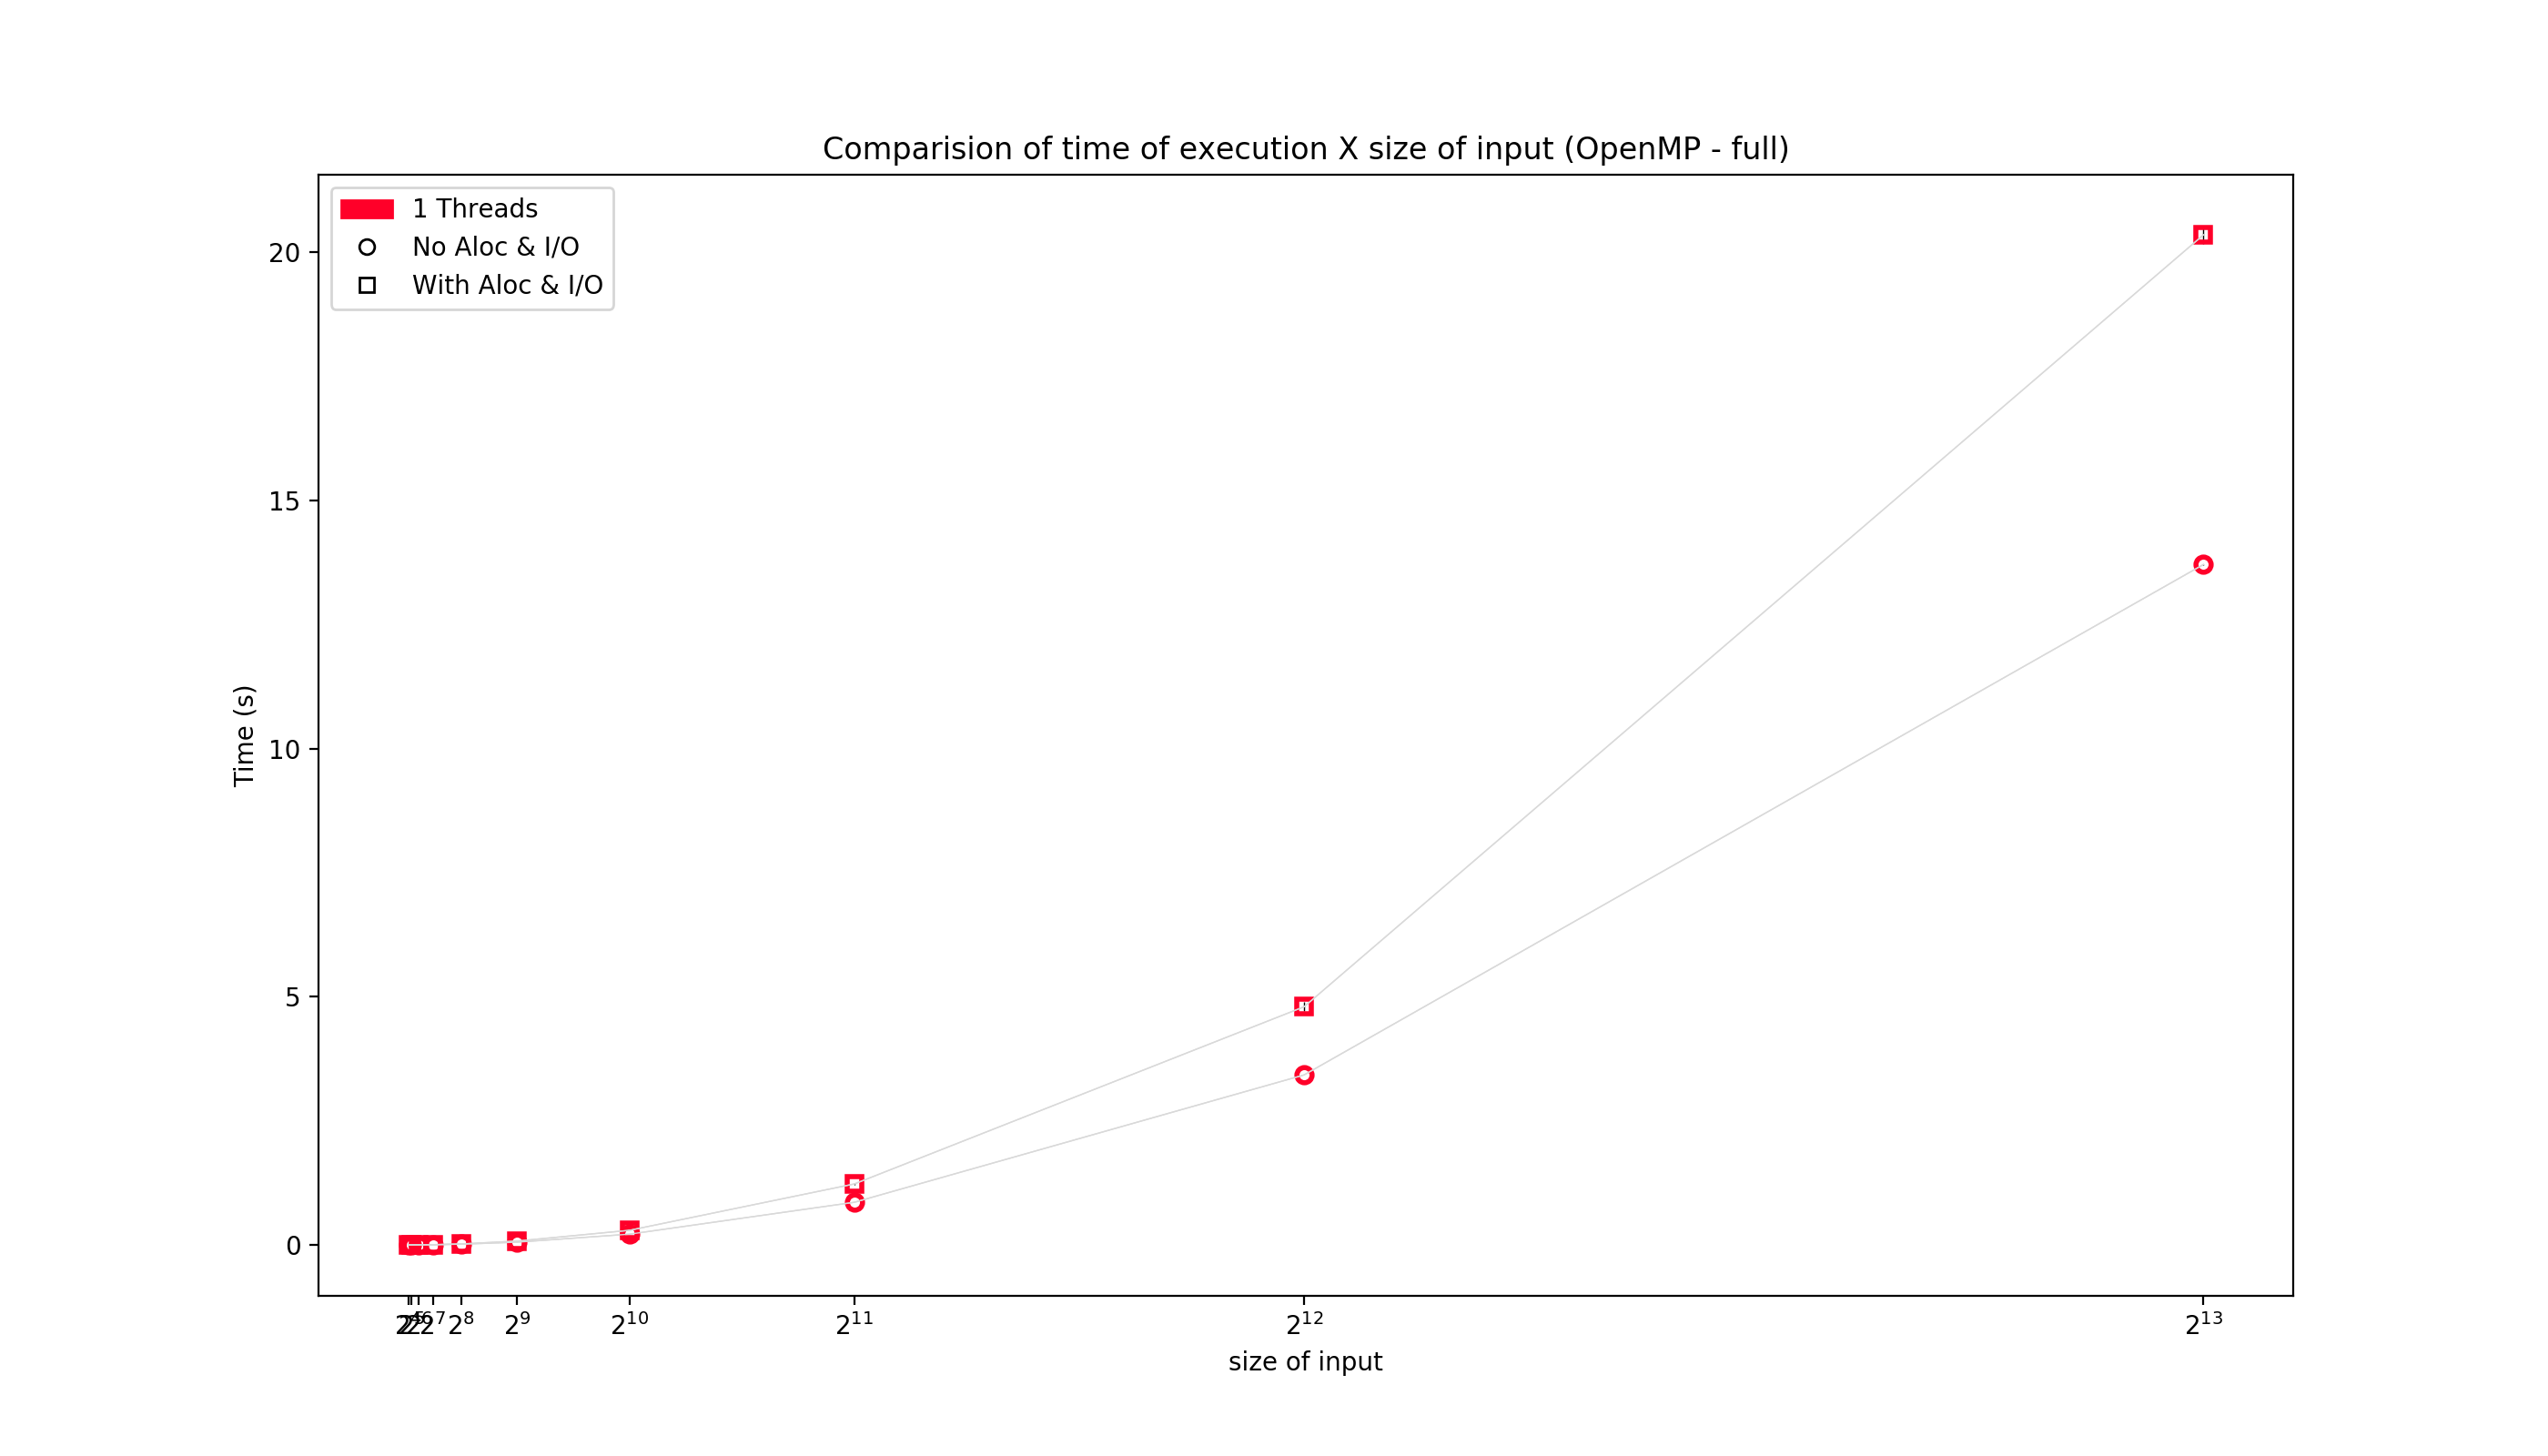
\includegraphics[scale=.60]{seq_comp/compare_timeXsize_full_OpenMPpng.png}}
\end{figure}

Como esperado o tempo do programa sem alocação e sem comandos de leitura e escrita é consideravelmente menor que a versão com. Nas demais regiões o comportamento se repete:

\begin{figure}[H]
    \makebox[\textwidth][c]{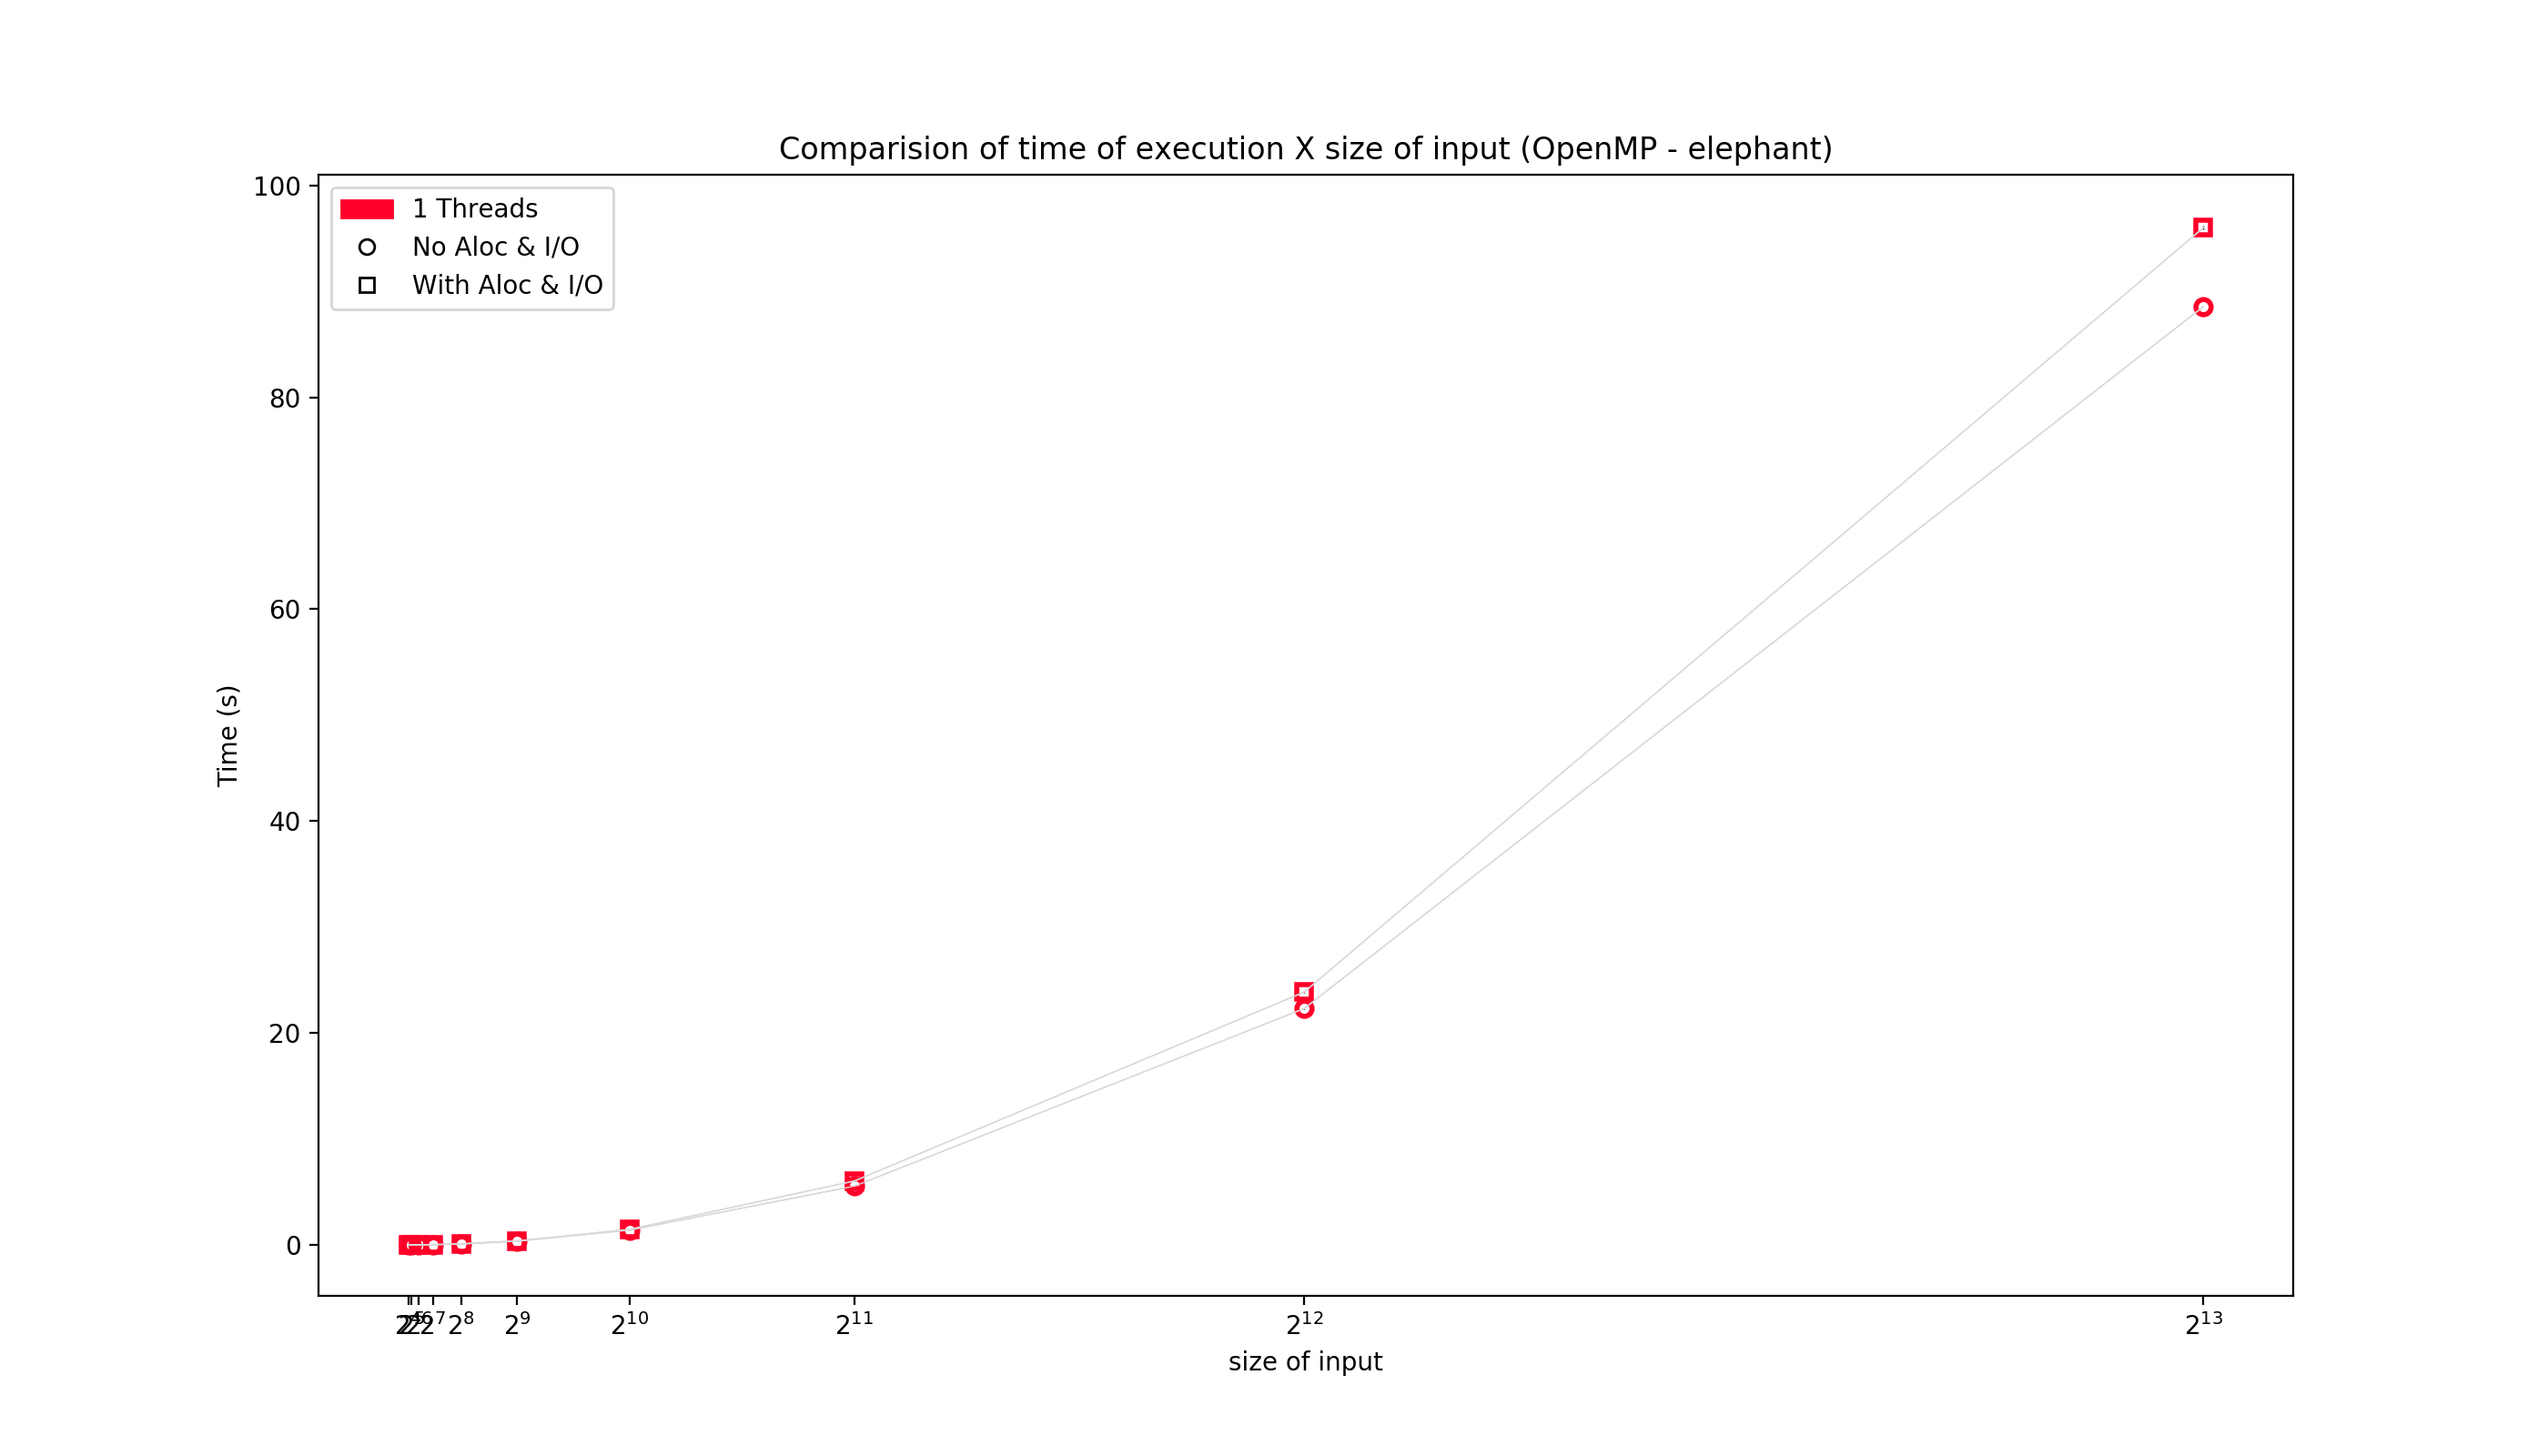
\includegraphics[scale=.50]{seq_comp/compare_timeXsize_elephant_OpenMPpng.png}}
\end{figure}
\begin{figure}[H]
    \makebox[\textwidth][c]{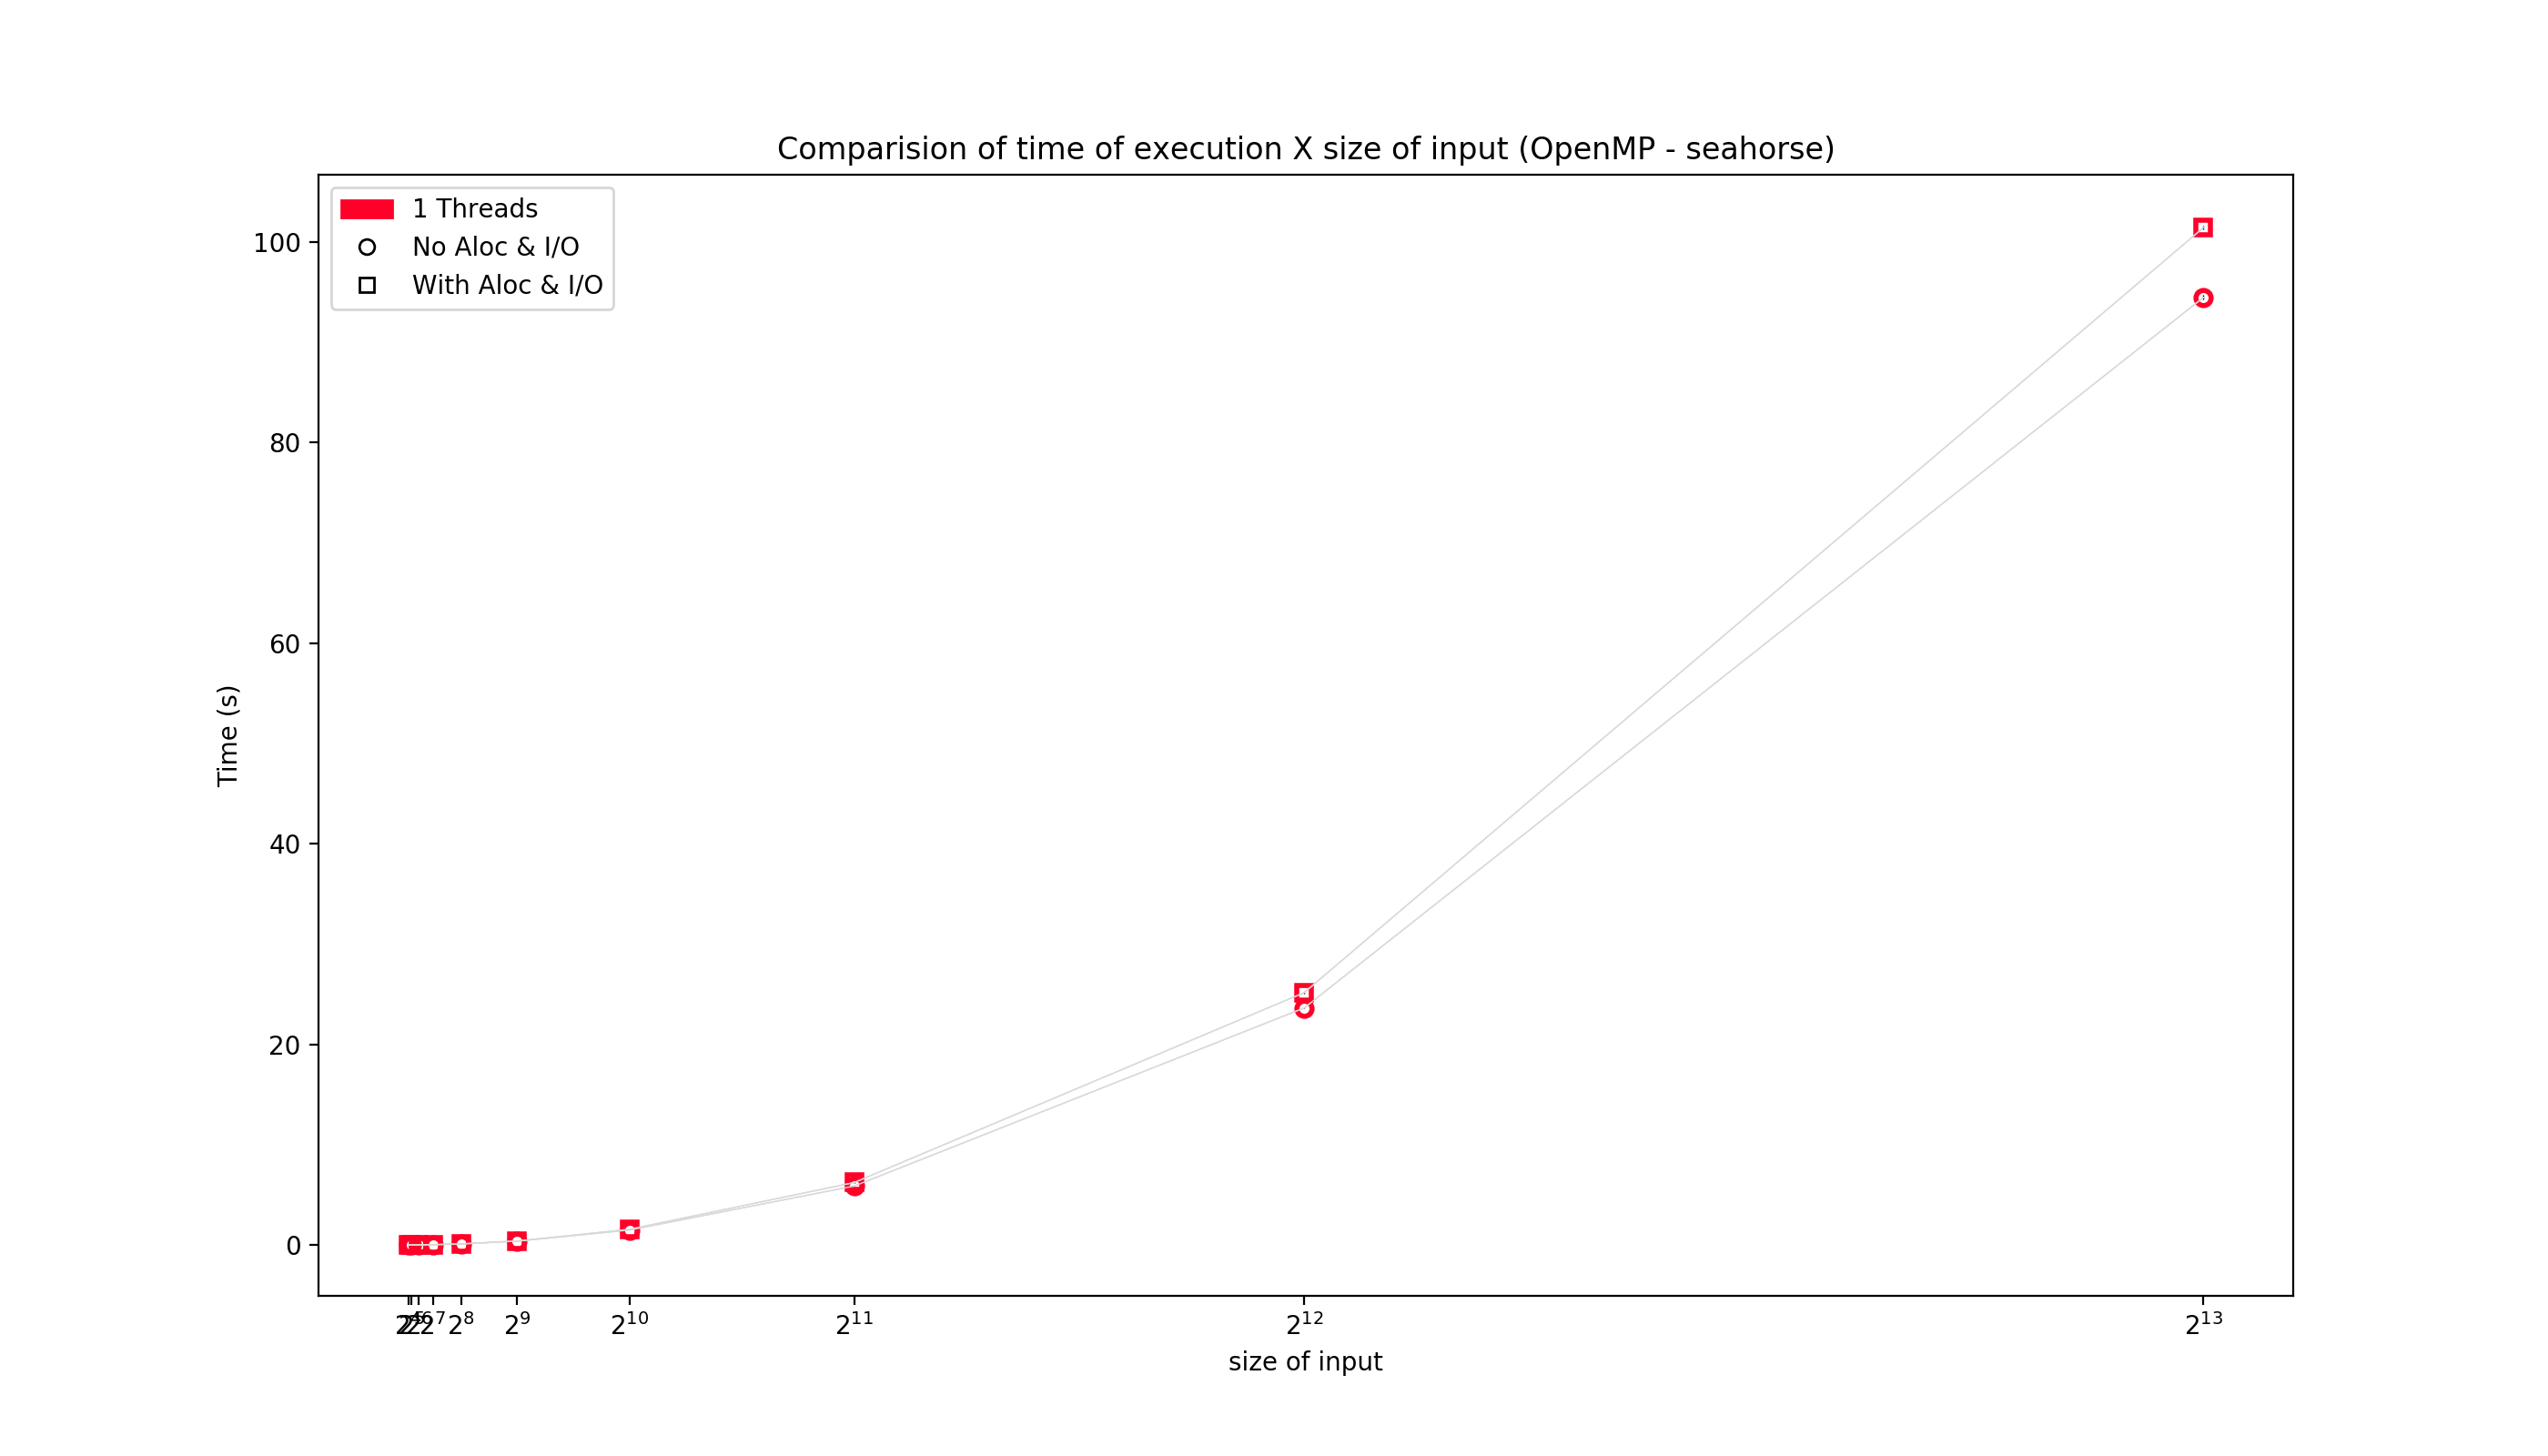
\includegraphics[scale=.50]{seq_comp/compare_timeXsize_seahorse_OpenMPpng.png}}
\end{figure}
\begin{figure}[H]
    \makebox[\textwidth][c]{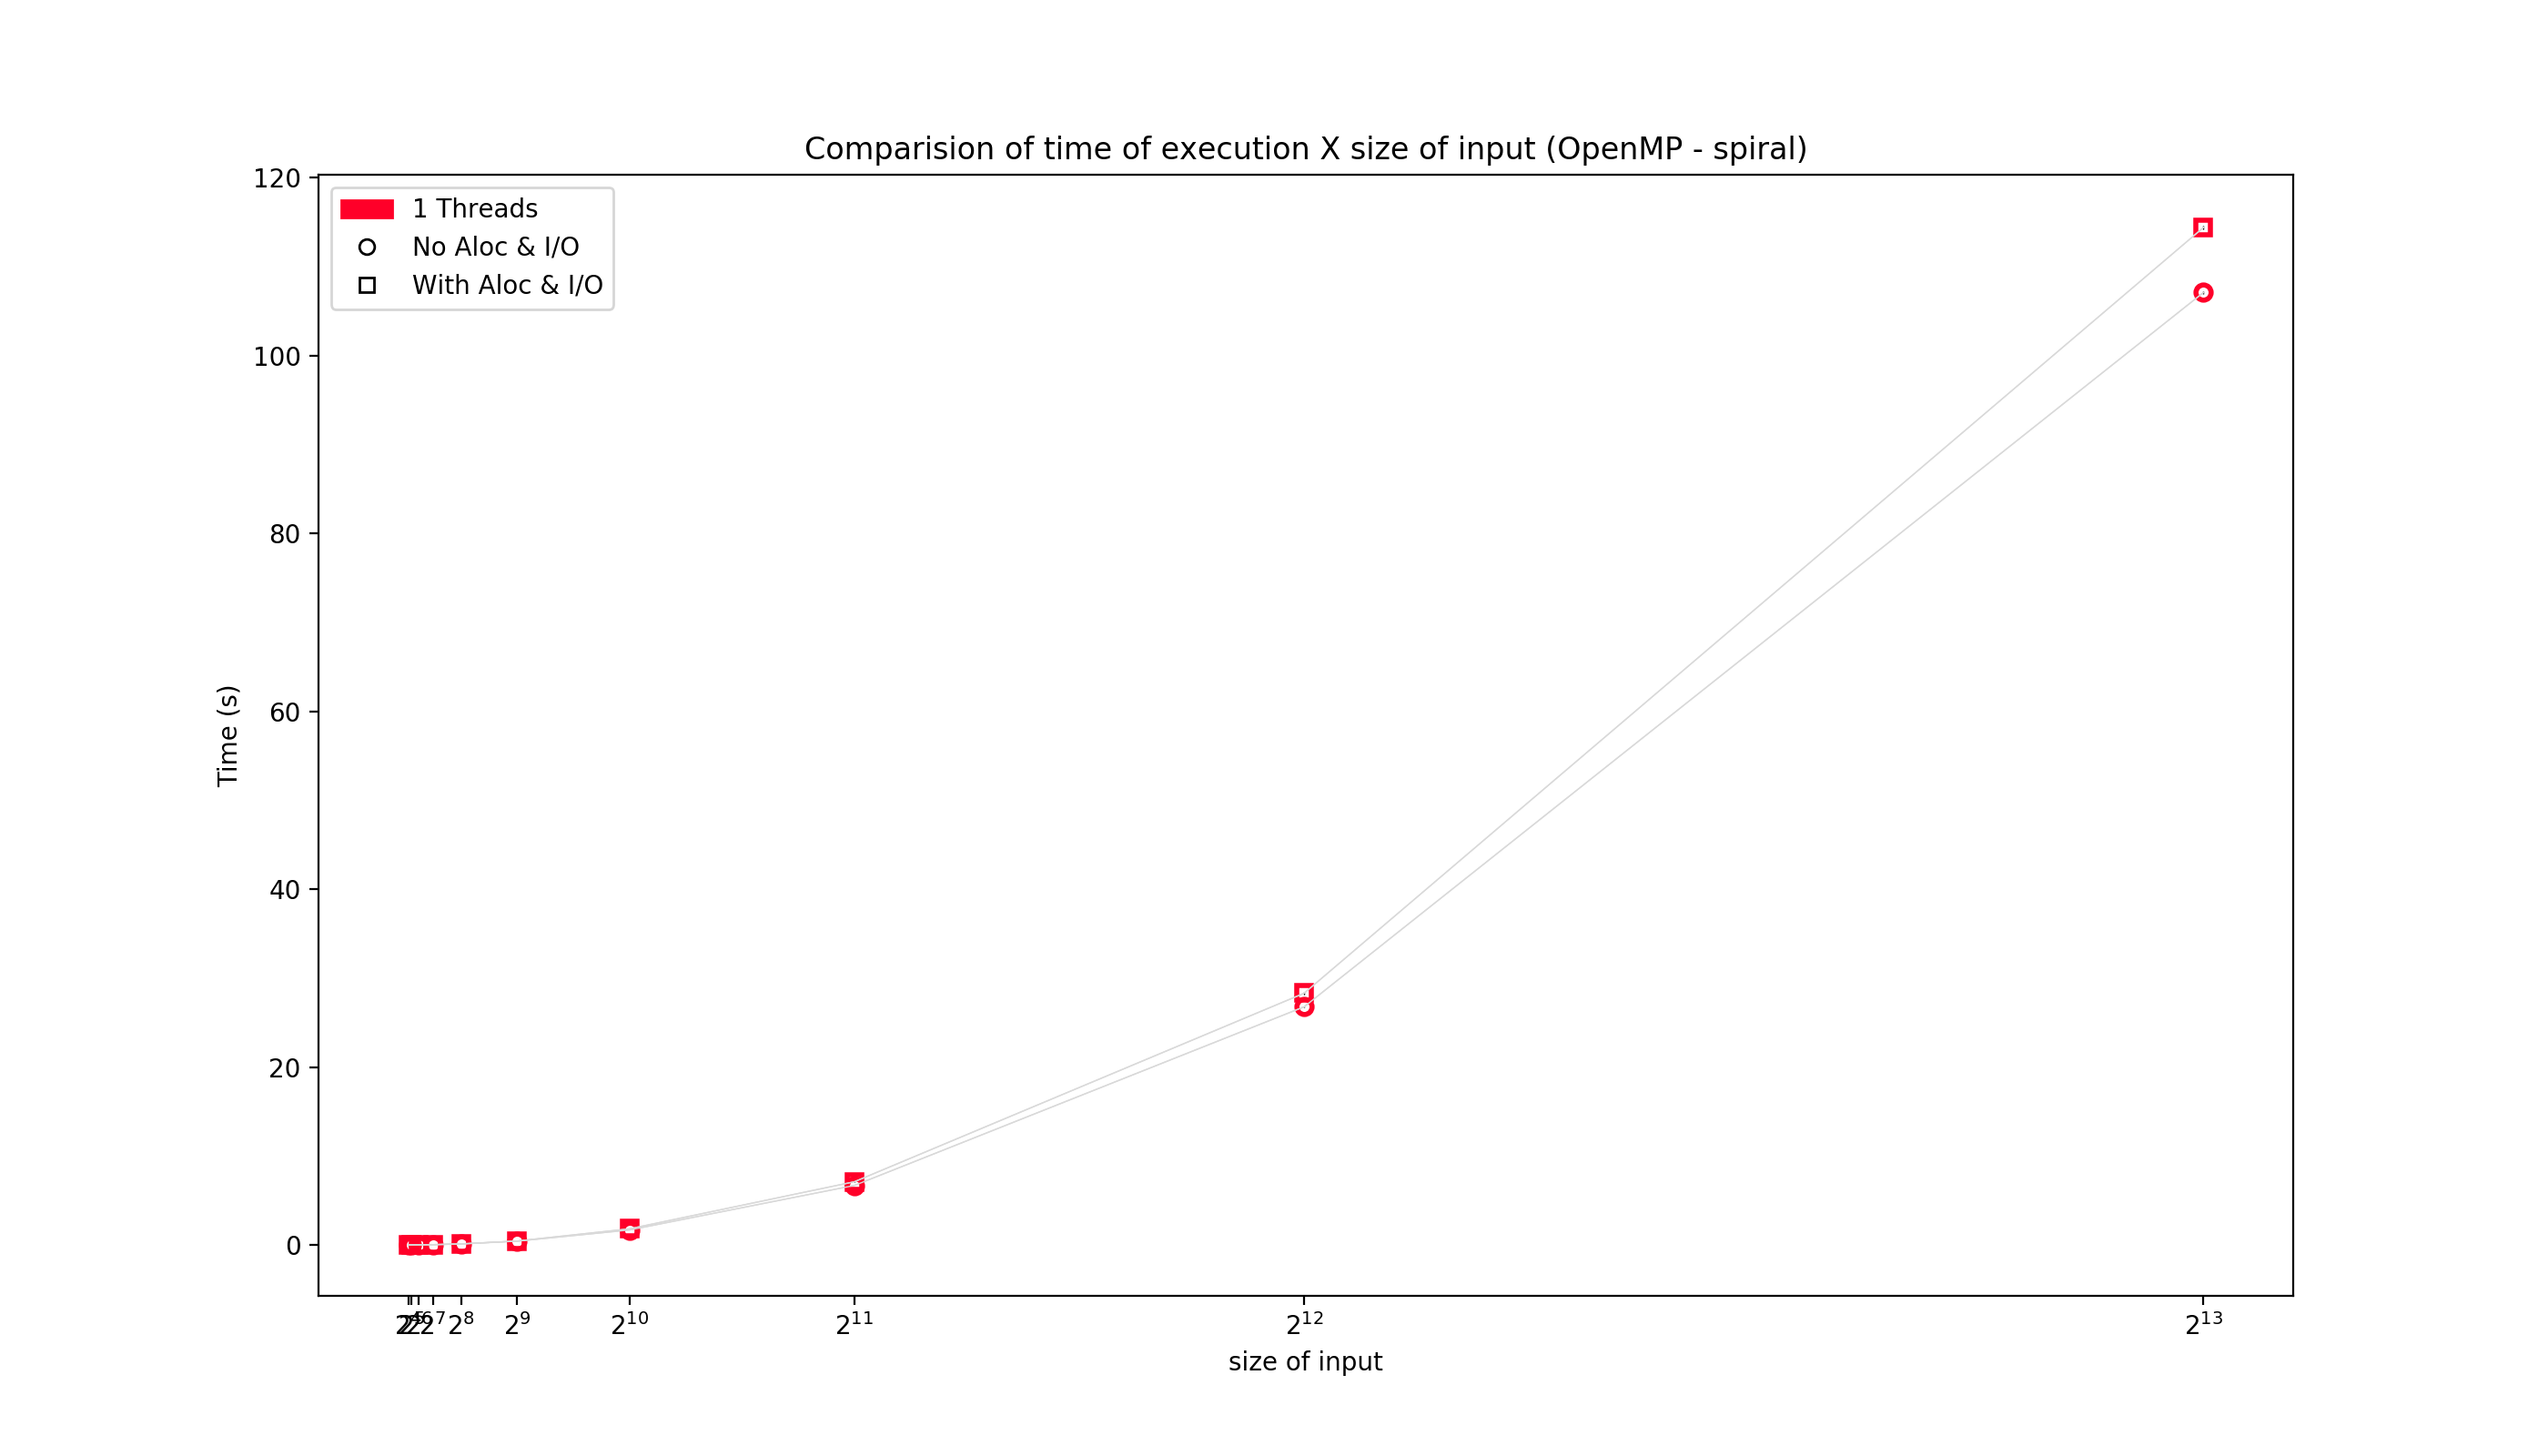
\includegraphics[scale=.50]{seq_comp/compare_timeXsize_spiral_OpenMPpng.png}}
\end{figure}

Nota-se que o tempo em cada região é diferente, pois em cada região pode haver mais cálculos de pontos com mais interações. Notemos ainda que a diferença de tempo para cada tamanho de entrada se mantem mesmo mudando-se as regiões. Por exemplo, a versão sem alocação dinamica e sem operações de leitura e escrita executa cerca de 10 segundos mais rapido que a versão com, dado a entrada de tamanho $2^(13)$, independente da região. Isso ocorre, pois comandos de leitura e escrita e alocação dinamica, dependem do tamanho da entrada e independem do número de interações do cálculo para determinado ponto.

Para cada implementação também vemos que o tempo para calcular a região Full foi bastante menor que para as demais regiões:

\begin{figure}[H]
    \makebox[\textwidth][c]{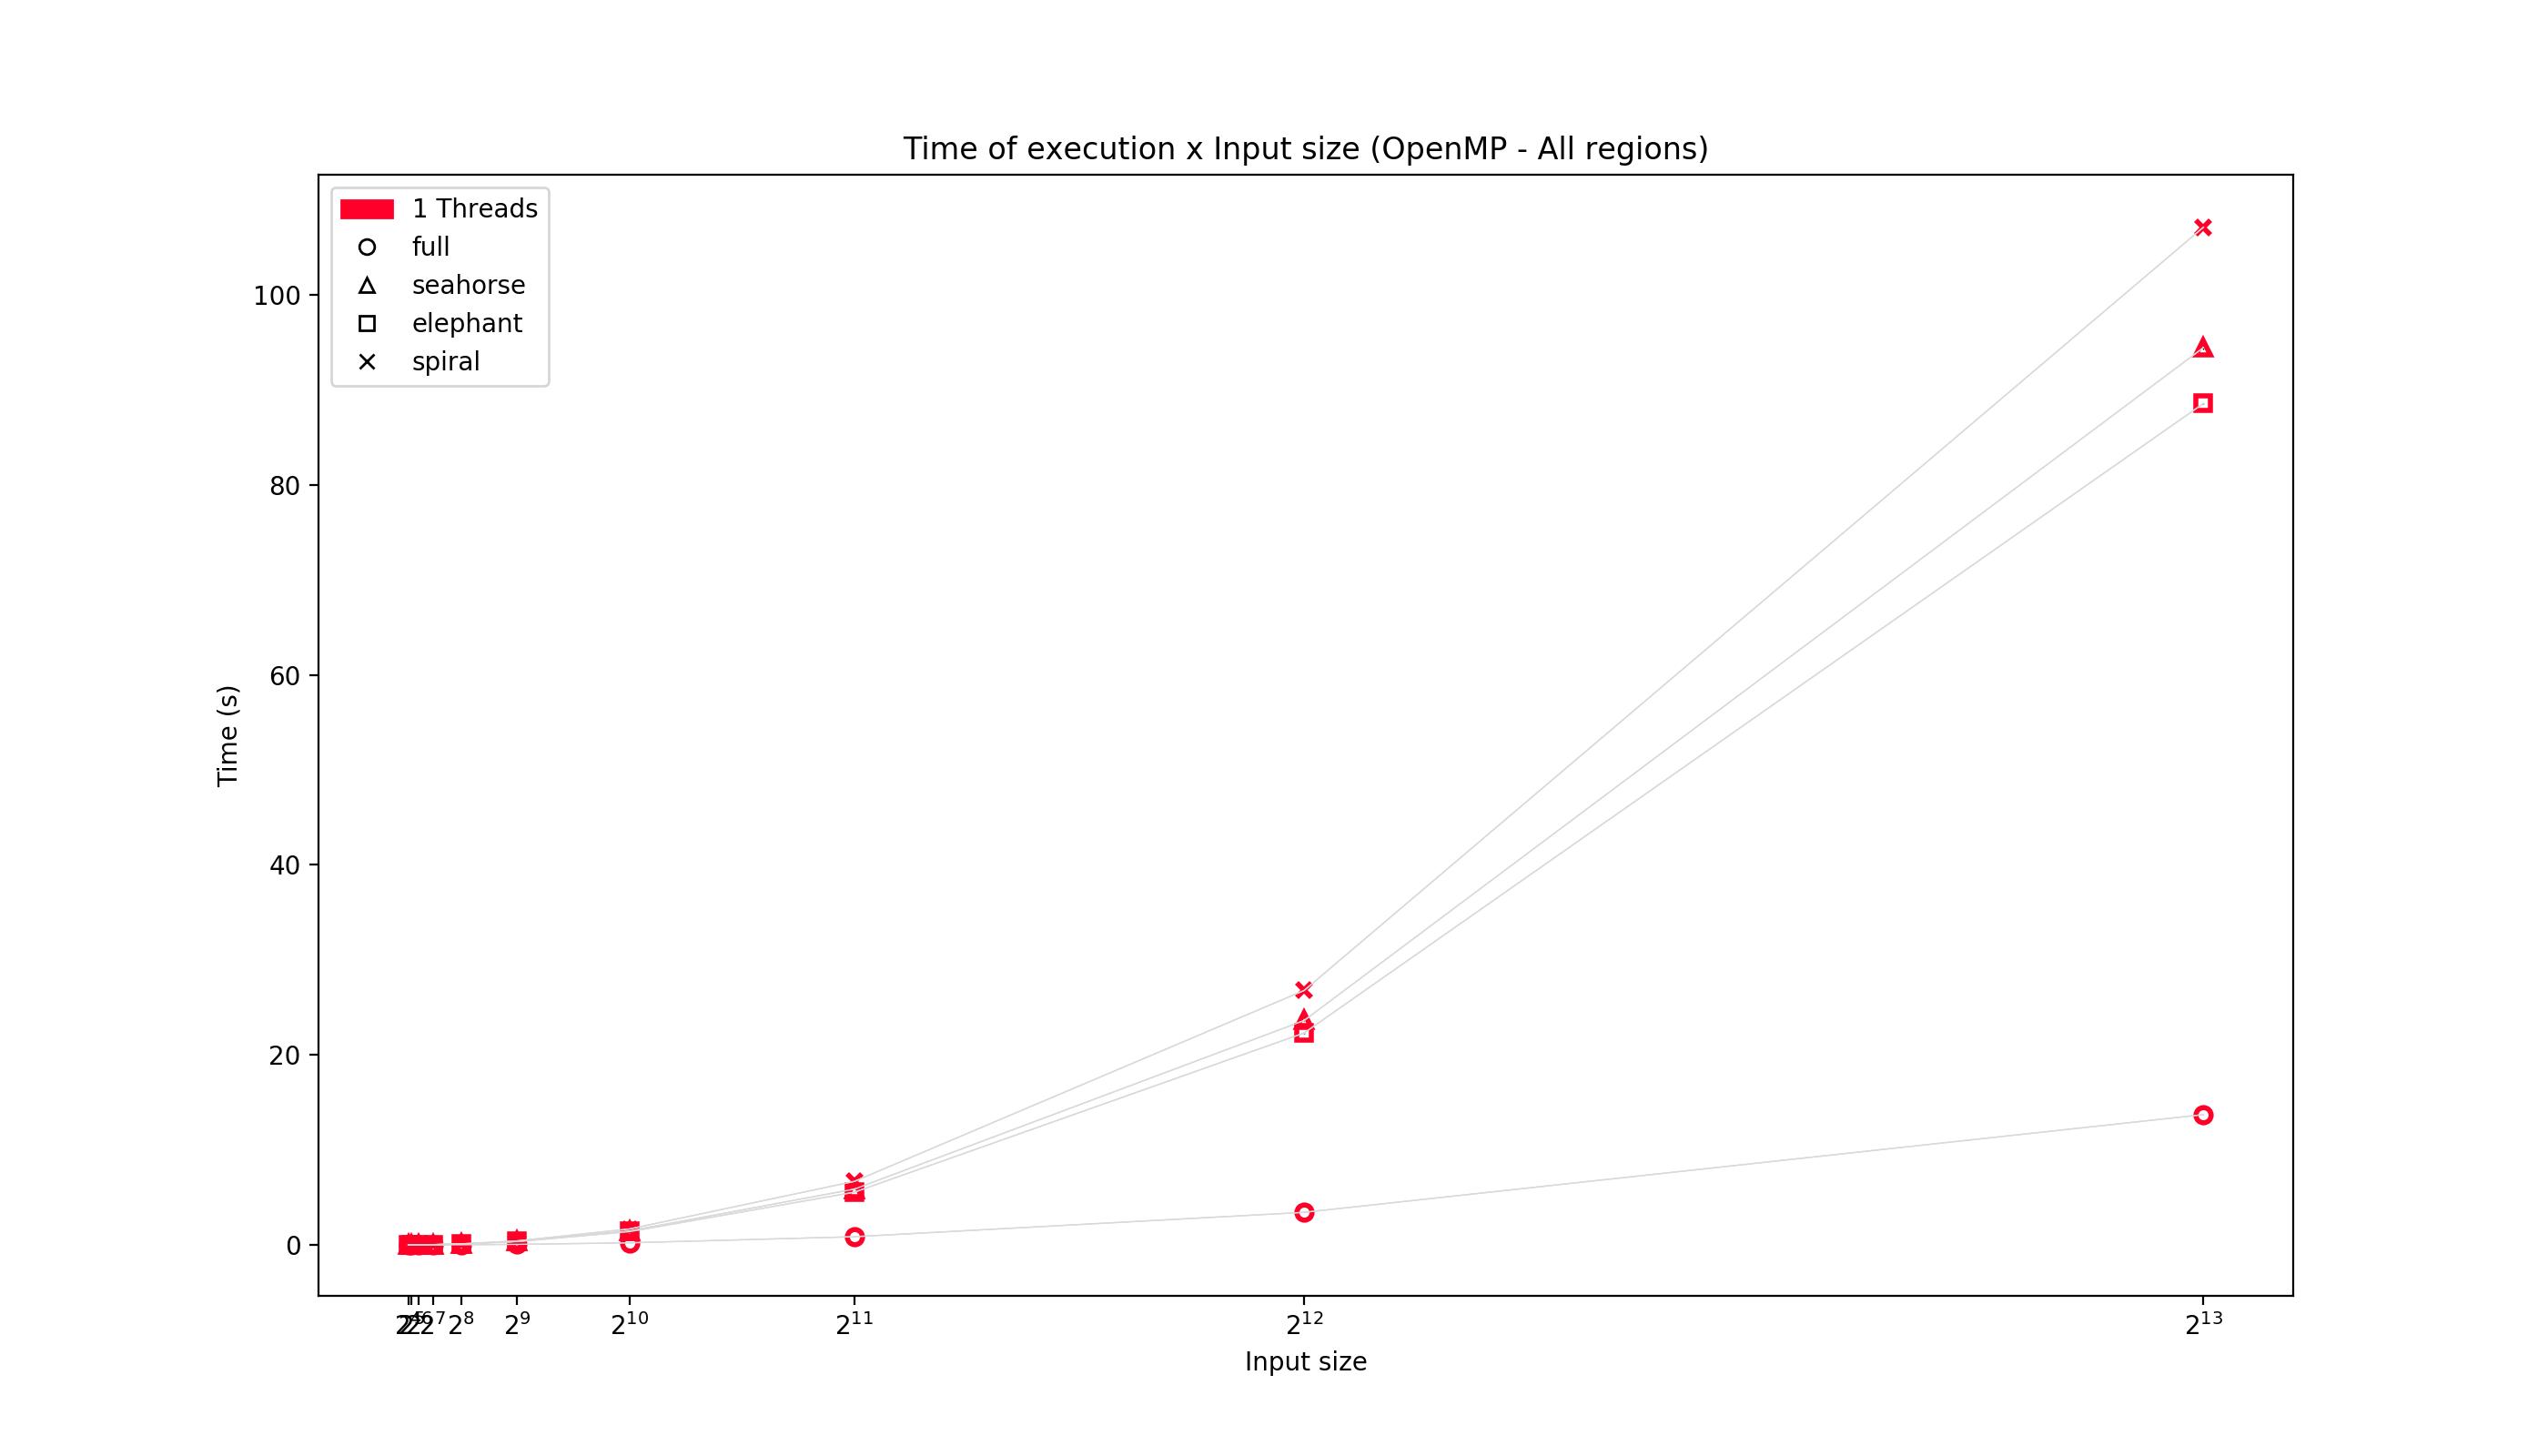
\includegraphics[scale=.50]{seq_no/all_timeXsize_OpenMPpng.png}}
    \caption{Implementação sem Operações de leitura e escrita e sem alocação de memória}
\end{figure}

\begin{figure}[H]
    \makebox[\textwidth][c]{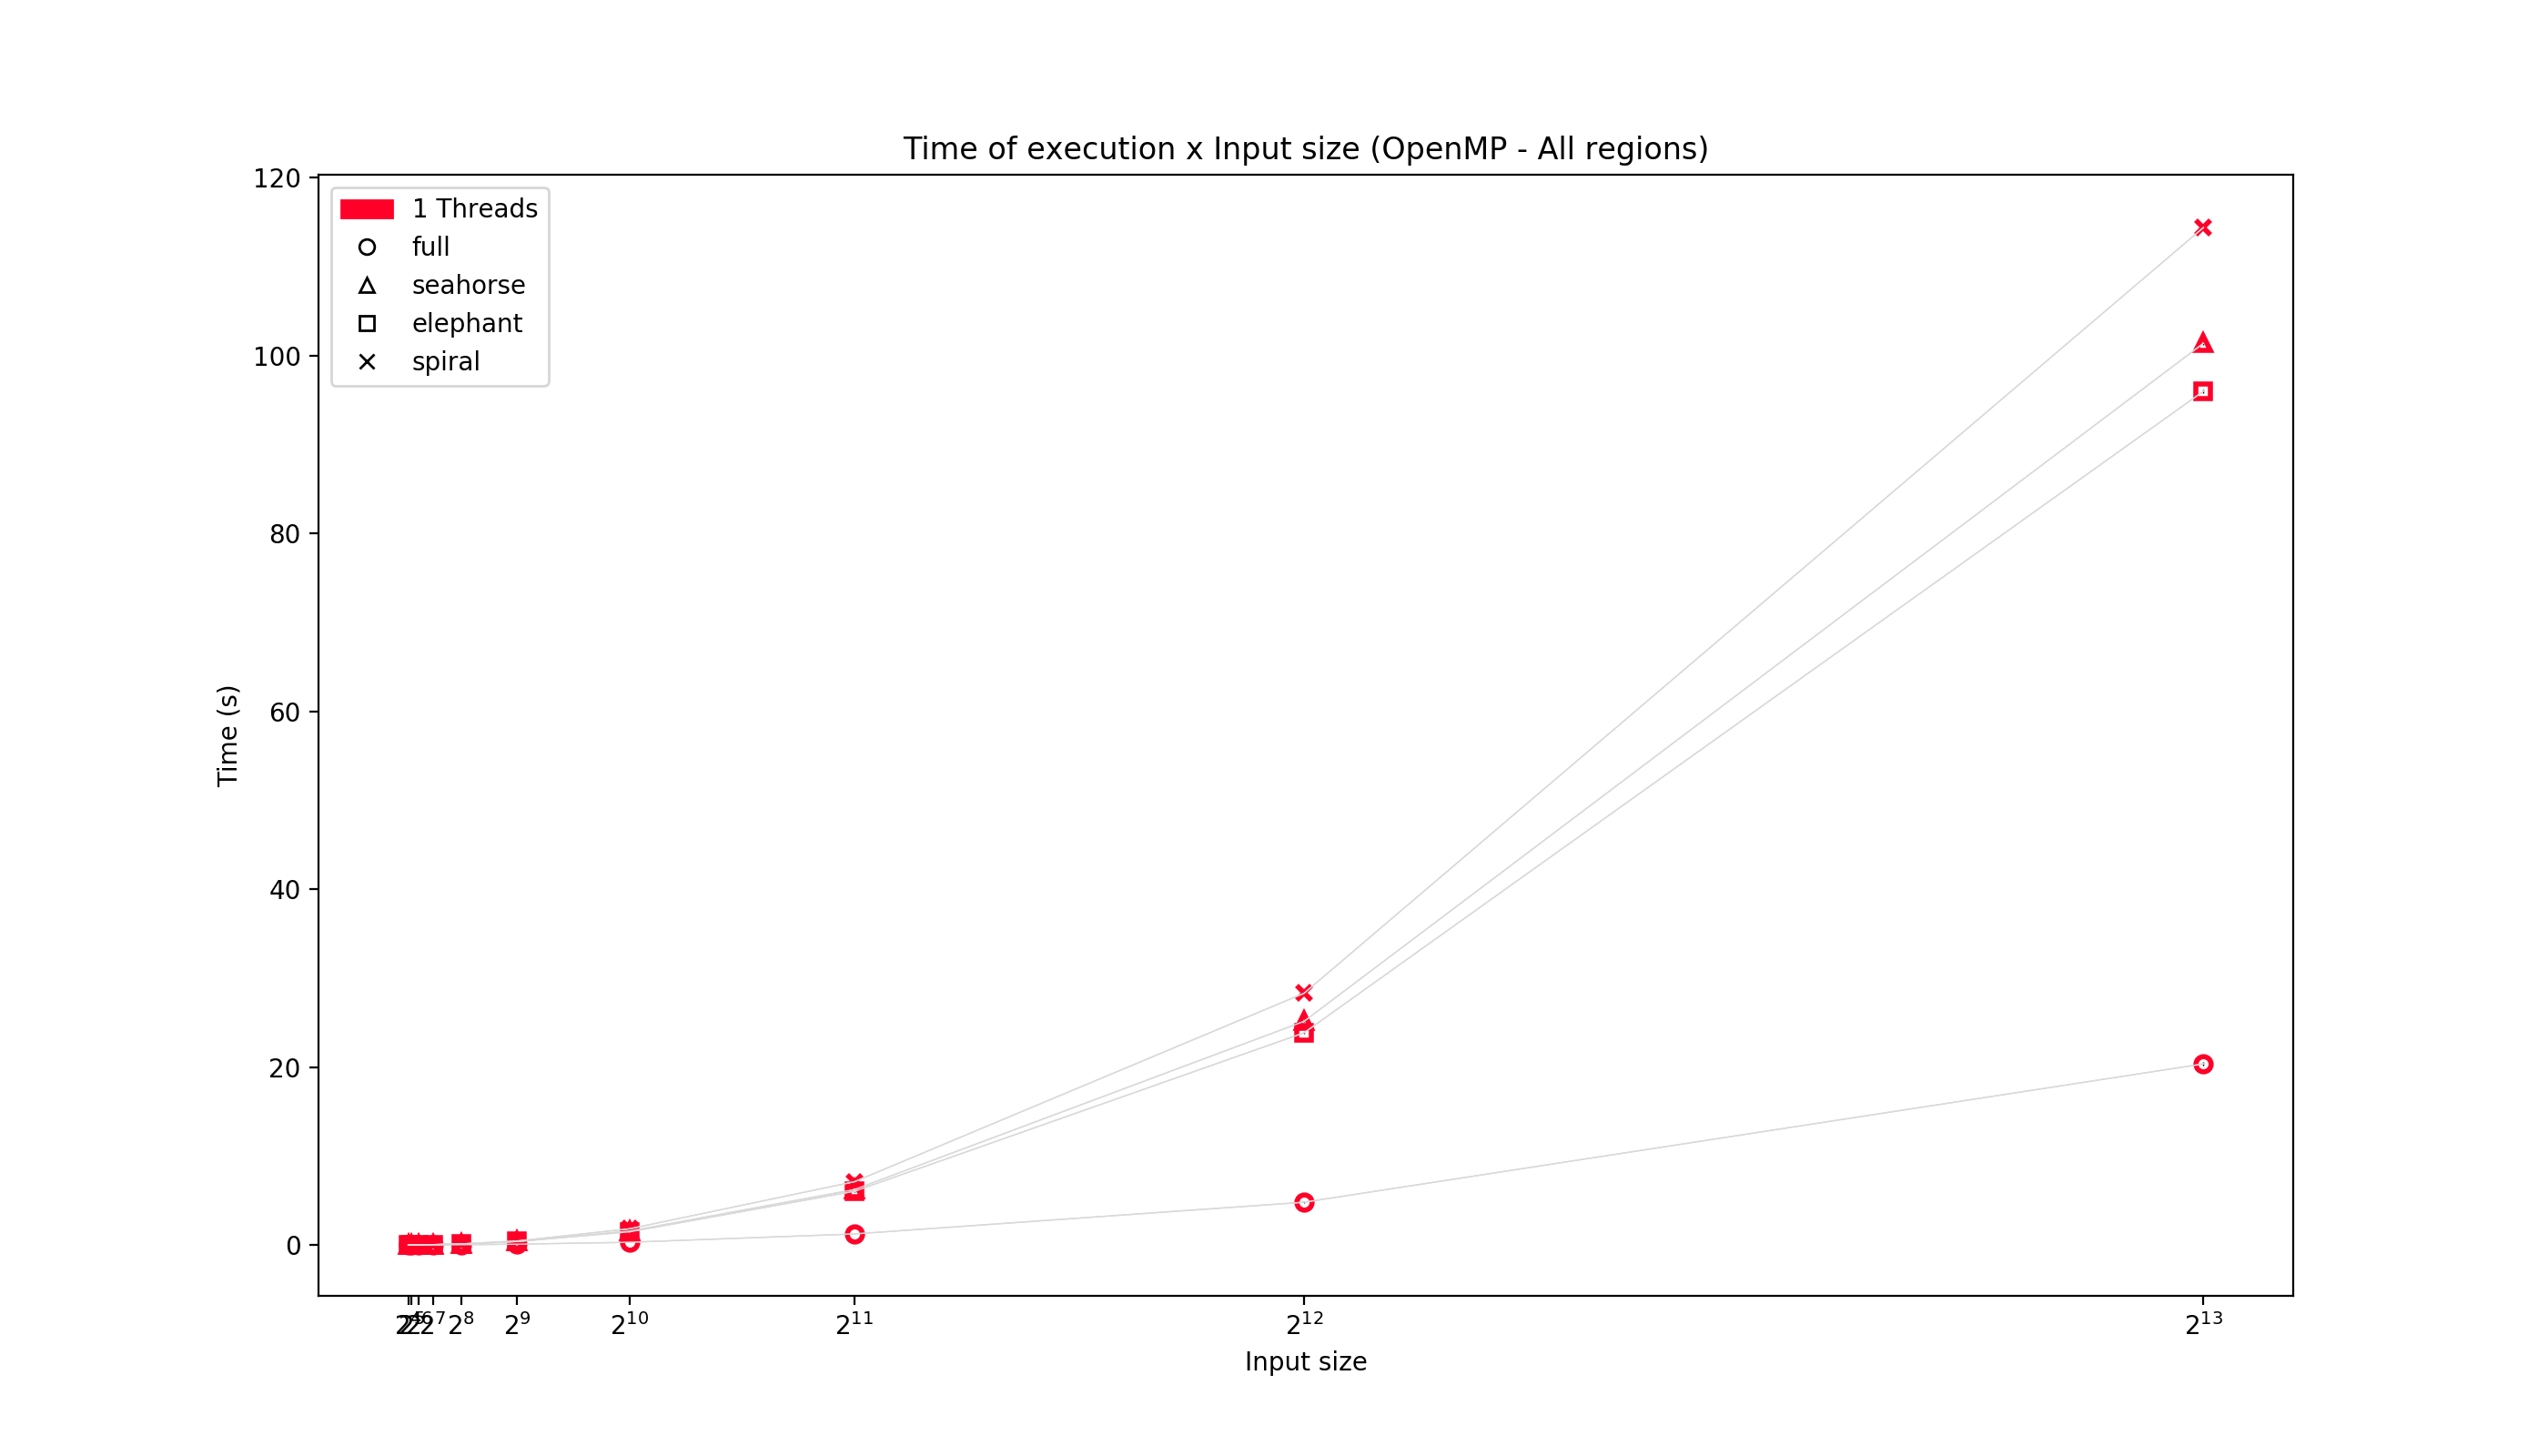
\includegraphics[scale=.50]{seq_with/all_timeXsize_OpenMPpng.png}}
    \caption{Implementação com Operações de leitura e escrita e com alocação de memória}
\end{figure}

%%%%%%%%%%%%%%%%%%%%% PTHREADS %%%%%%%%%%%%%%%%%%%%%%%%%%%%%%
\newpage
\section{Código em Pthreads}
Utilizamos duas diferentes abordagens para paralelizar o código com
o uso de pthreads, tentando se aproximar ao comportamento do OpenMP e 
suas diretivas {\em omp parallel for schedule (dynamic)} e {\em omp 
parallel for schedule (static)}. As diferenças de funcionamento dos 
dois códigos está na maneira em que o trabalho é dividido e como ele é
distribuído para cada thread.

\subsection{Implementação com Divisão Estática}
Chamamos de implementação com divisão estática a versão do nosso 
código em pthreads no qual o trabalho é dividido em $n$ pedaços de mesmo 
tamanho, e cada pedaço é dado a uma thread. Chamamos essa implementação
de estática porque cada thread recebe apenas um bloco de trabalho,
pré-determinado pela divisão feita, que será processado do começo ao
fim (no escopo da thread) pela mesma thread.

Para implementar esse código, precisamos apenas construir uma estrutura
de dados que era capaz de guardar um bloco de pixels a ser calculado.
Dado essa estrutura, basta criar uma thread para cada bloco de trabalho,
que por sua vez deve calcular os pixels correspondentes e atualizar o 
buffer de cores.

Devemos observar que essa implementação pode implicar em threads ociosas
enquanto outras estão trabalhando. Como a quantidade de iterações
necessárias para se calcular o valor de um pixel varia, é possível que
um bloco de pixels seja calculado muito mais rápido do que outro; 
imagine por exemplo um bloco onde cada ponto calculado diverge 
rapidamente e outro bloco onde isso não acontece. Portanto, como a 
divisão de trabalho é estática, é provável que uma thread termine seu
trabalho muito antes de outra, o que significa em um uso não muito bom
de recursos da máquina.

Uma possível solução para esse problema seria o aumento no número de 
threads, o que cria uma fragmentação maior do trabalho. Essa 
fragmentação ameniza o problema anterior porque divide mais o trabalho,
deixando menor a diferença de tempo necessário para se calcular cada 
parte. Entretanto, criar um número excessivo de threads pode dar mais
trabalho ao escalonador do sistema operacional, que deve lidar com 
várias linhas de processamento.

\begin{figure}[!ht]
    \centering
    \begin{tabular}{c c}
        \subfigure[] {\scalebox{.35}{
            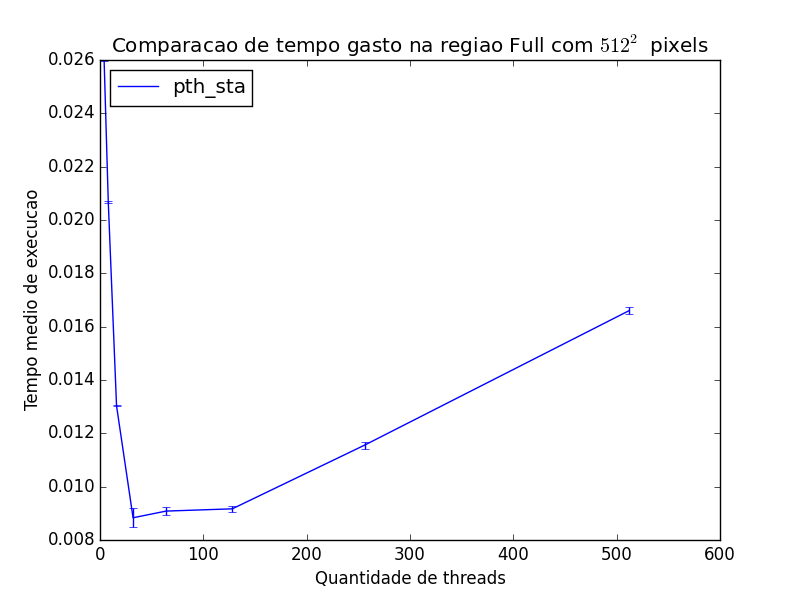
\includegraphics{pthread_numthreads/time_x_thread_numpth_sta_n512.png}}
            \label {fig:higher_thread_num:A}
        }
        &
        \subfigure[] {\scalebox{.35}{
            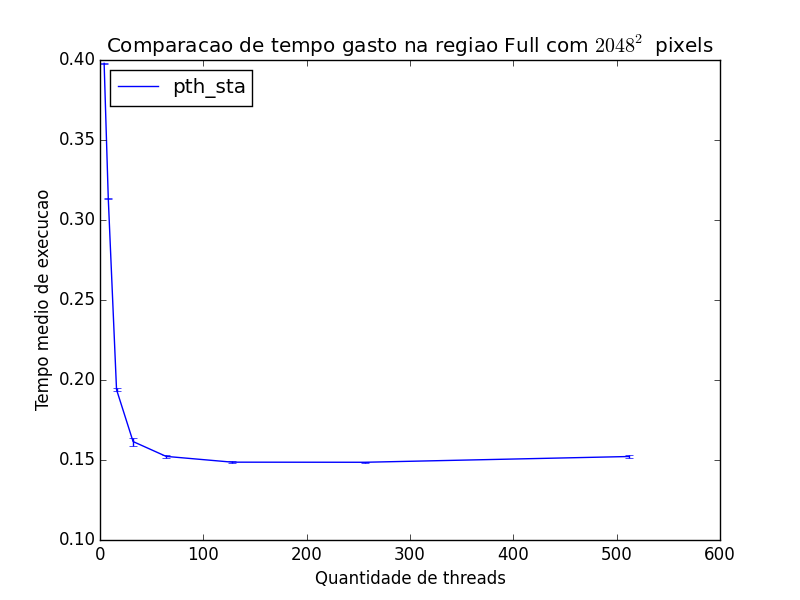
\includegraphics{pthread_numthreads/time_x_thread_numpth_sta_n2048.png}}
            \label {fig:higher_thread_num:B}
        }

    \end{tabular}
    \caption{É possível notar em ambas figuras que o aumento do número
    de threads de fato diminui o tempo de execução do programa. No 
    gráfico \ref{fig:higher_thread_num:A} fica evidente que o tempo 
    gasto no controle das threads pode afetar o tempo de execução do
    programa.}
    \label{fig:higher_thread_num} 
\end{figure}

\subsection{Implementação com Divisão Dinâmica}
A implementação dinâmica do nosso programa também divide o trabalho em
$n$ pedaços, entretanto agora $n$ não é mais, necessariamente o número
de threads disponíveis. Após dividir o trabalho em pedaços, o nosso 
programa agora é capaz de, dinamicamente, delegar blocos de pixels a 
cada thread. Portanto, agora diminuímos o problema de threads ociosas,
porque podemos dividir mais os blocos de trabalho e sempre que uma 
thread termina um bloco, podemos dar a ela um novo bloco para computar 
(desde que ainda haja trabalho a ser feito).

Veja abaixo um pseudo-código para esse programa:
\begin{algorithmic}[1]
\Function{ComputeMandelbrot}{}
    \State $S \gets $ lista de nacos de todos os pixels
    \While{$S \neq \emptyset$}
        \State $chunk \gets S$.popChunk ()
        \State Espere {\em alguma} thread estar livre
        \ForAll{Threat $T$}
            \If{$T$ está livre}
                \State $T$.compute ($chunk$)
            \EndIf
        \EndFor
    \EndWhile 
    \EndFunction
\end{algorithmic}

A implementação desse código é um pouco mais complicada, porque depende,
além da estrutura de dados já usada na implementação estática, de um 
maior controle de concorrência. O conceito principal utilizado é o de 
{\em condition variable}, que nos permite colocar a linha principal de
execução em espera, enquanto as threads calculam os pixels, para voltar
a ser executada quando alguma thread estiver livre.

\begin{figure}[!ht]
    \centering
    \begin{tabular}{c c}
        \subfigure[] {\scalebox{.35}{
            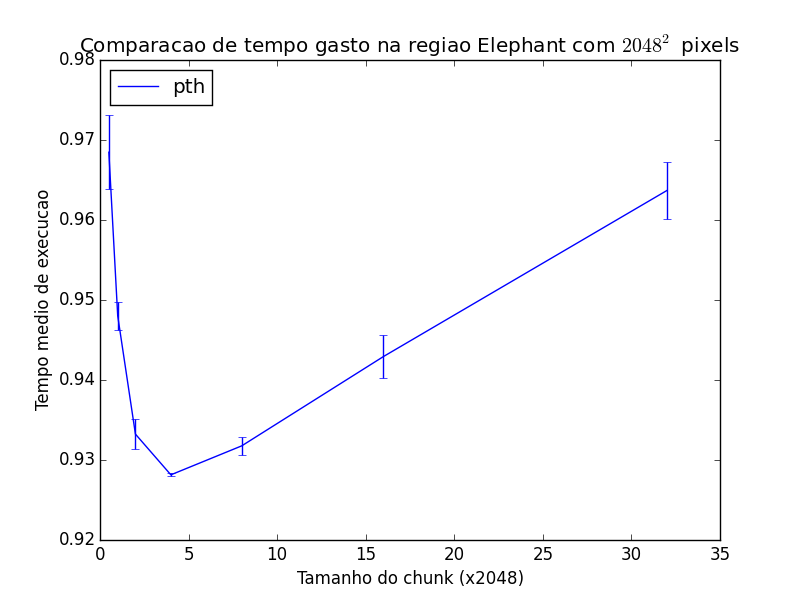
\includegraphics{pthread_chunk/time_x_chunk_sizepth2048elephant.png}}
            \label {fig:pthreads_chunk_size:A}
        }
        &
        \subfigure[] {\scalebox{.35}{
            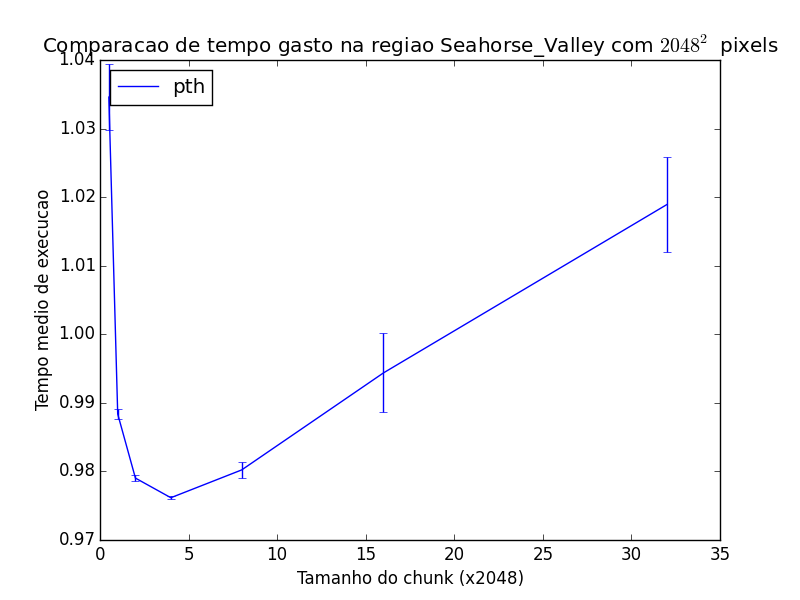
\includegraphics{pthread_chunk/time_x_chunk_sizepth2048seahorse_valley.png}
        }
            \label {fig:pthreads_chunk_size:B}
        }
        \\
        \subfigure[] {\scalebox{.35}{
            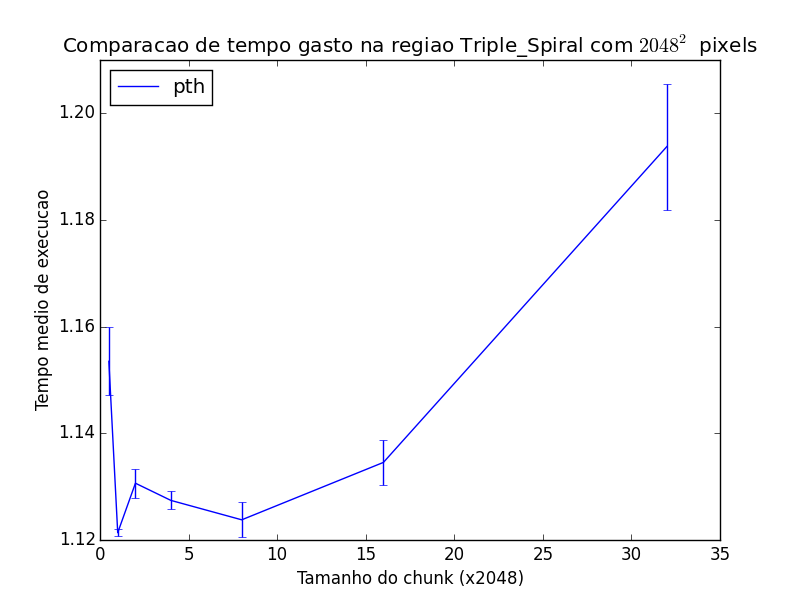
\includegraphics{pthread_chunk/time_x_chunk_sizepth2048triple_spiral.png}}
            \label {fig:pthreads_chunk_size:C}
        }
        &
        \subfigure[] {\scalebox{.35}{
            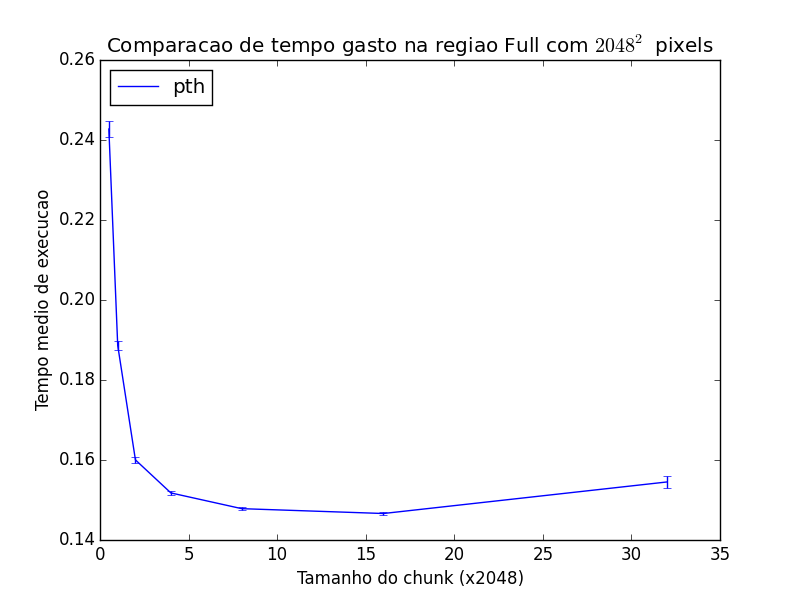
\includegraphics{pthread_chunk/time_x_chunk_sizepth2048full.png}}
            \label {fig:pthreads_chunk_size:D}
        }
        
    \end{tabular}
    \caption{Verificamos empiricamente que definir o tamanho do chunk 
        como  o tamanho do lado da imagem traz bons resultados para o
        tempo de execução.}
    \label{fig:pthreads_chunk_size} 
\end{figure}


Diminuído o problema de threads ociosas, é esperado que essa 
implementação seja mais rápida do que a anterior, porém, é necessário 
notar que o nosso código ficou mais complexo, e exige mais recursos
computacionais para o controle das threads. Esse tempo pode ser 
prejudicial se o tamanho do chunk for pequeno, pois nessa situação
há muitas trocas de chunks em cada thread, fazendo com que a maior parte
do tempo de processamento seja gasto no controle das threads. Por outro
lado, se temos chunks muito grandes, o tempo gasto deve aumentar, porque
caímos novamente no problema da implementação static, onde o trabalho 
não era bem dividido. Depois de fazer alguns testes, verificamos 
que definir o tamanho do chunk igual a quantidade de pixels em uma linha
da imagem nos dava bons resultados; inclusive, esse foi o mesmo valor 
adotado em nossa implementação com OpenMP.

\begin{figure}[!h]
    \centering
    \begin{tabular}{c c}
        \subfigure[] {\scalebox{.35}{
            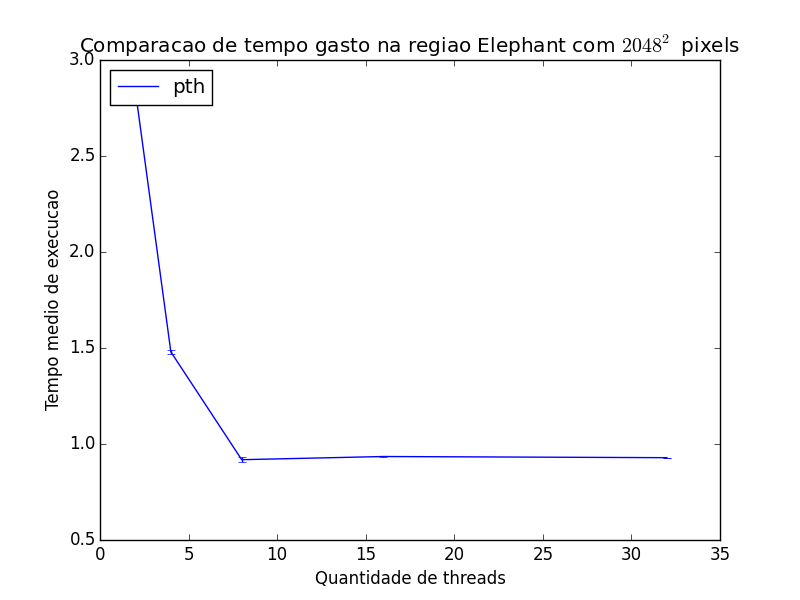
\includegraphics{pthread_numthreads/time_x_thread_numpth2048_elephant.png}}
            \label {fig:pthreads_num_threads:A}
        }
        &
        \subfigure[] {\scalebox{.35}{
        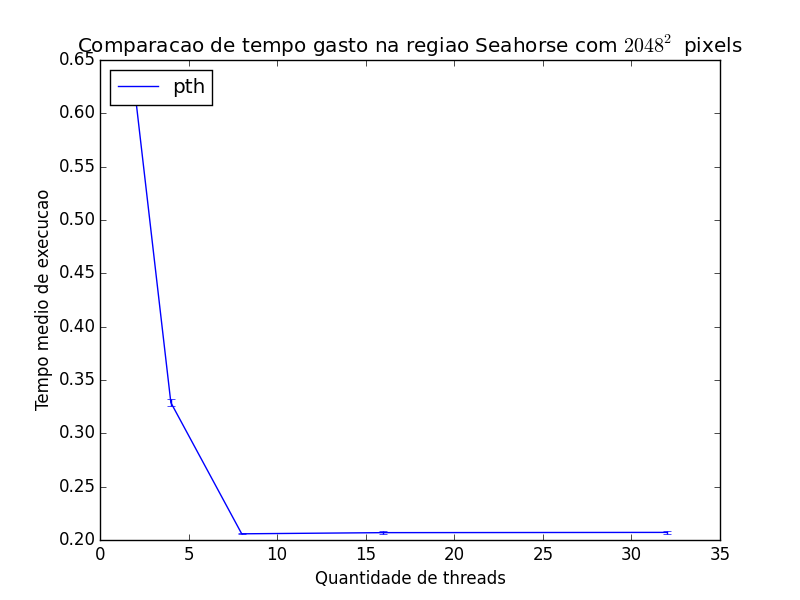
\includegraphics{pthread_numthreads/time_x_thread_numpth2048_seahorse.png}
        }
            \label {fig:pthreads_num_threads:B}
        }
        \\
        \subfigure[] {\scalebox{.35}{
            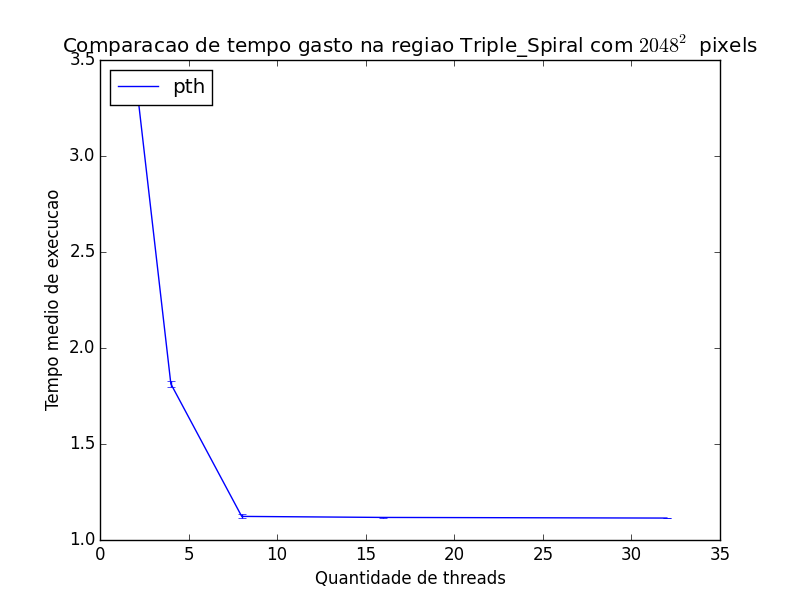
\includegraphics{pthread_numthreads/time_x_thread_numpth2048_triple_spiral.png}}
            \label {fig:pthreads_num_threads:C}
        }
        &
        \subfigure[] {\scalebox{.35}{
            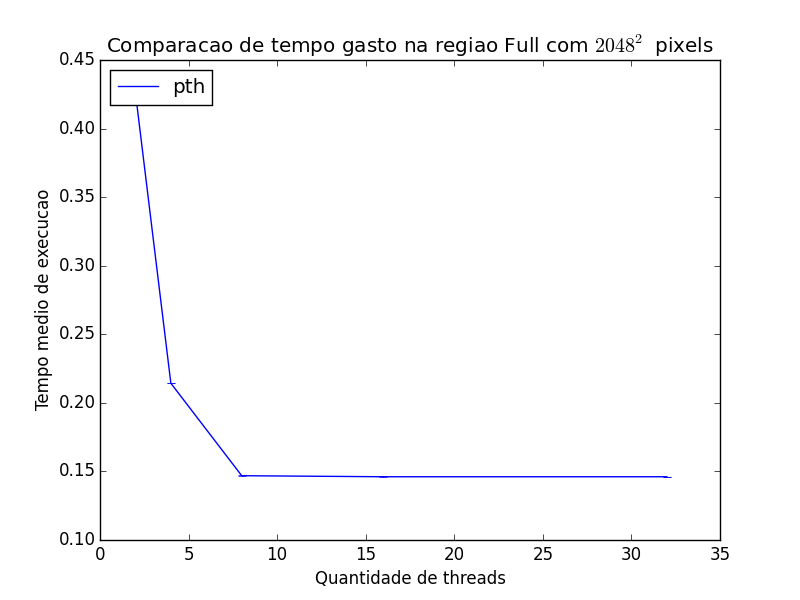
\includegraphics{pthread_numthreads/time_x_thread_numpth2048_full.png}}
            \label {fig:pthreads_num_threads:D}
        }
        
    \end{tabular}
    \caption{Podemos observar que existe uma saturação de melhora de 
    desempenho quando o número de threads atinge o número de cores (8)
    da máquina.}
    \label{fig:pthreads_thread_num} 
\end{figure}

Como distribuímos dinamicamente os blocos de trabalho, é esperado que
o aumento do número de threads não melhore o problema de threads 
ociosas, diferente do que vimos na implementação com divisão estática
e na figura \ref{fig:higher_thread_num}. A melhora com o aumento de 
threads deve vir unicamente do melhor uso da quantidade de cores da 
máquina, ou seja, a quantidade de threads deve melhorar o desempenho 
enquanto não foi maior do que o número de processadores da máquina.
De fato, observamos esse comportamento na figura 
\ref{fig:pthreads_thread_num}

Veja abaixo a comparação em consumo de tempo entre as duas 
implementações de paralelismo com Pthreads:
\begin{figure}[!h]
    \centering
    \begin{tabular}{c c}
        \subfigure[] {\scalebox{.35}{
            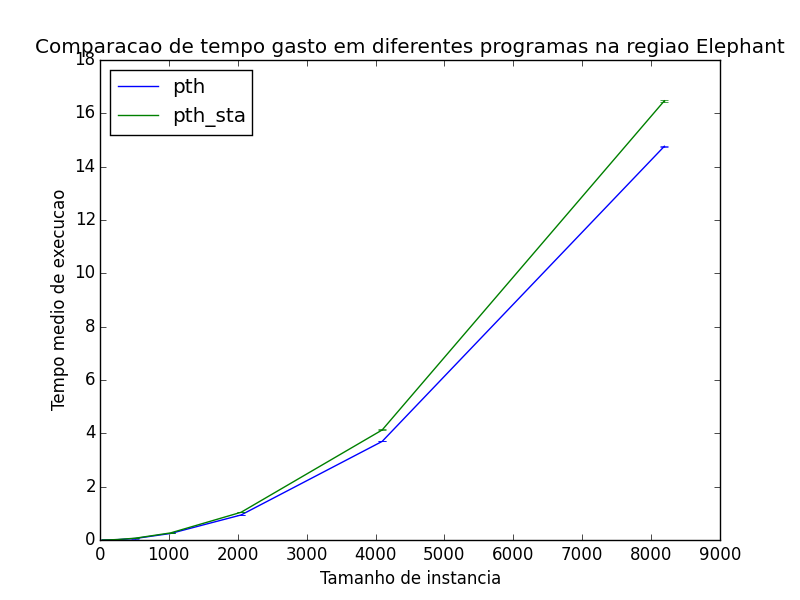
\includegraphics{pthread_din_sta/time_x_sizepth-pth_staelephant.png}}
            \label {fig:pthreads_din_sta:A}
        }
        &
        \subfigure[] {\scalebox{.35}{
        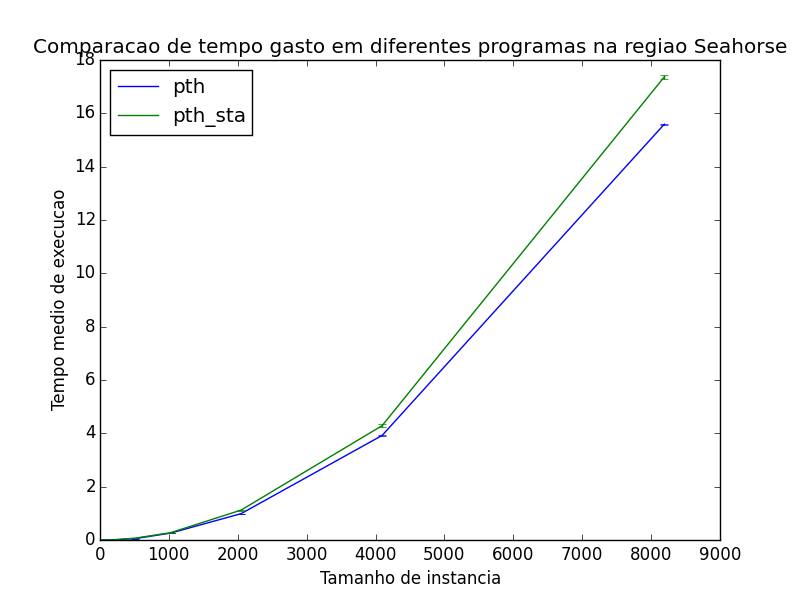
\includegraphics{pthread_din_sta/time_x_sizepth-pth_staseahorse.png}
        }
            \label {fig:pthreads_din_sta:B}
        }
        \\
        \subfigure[] {\scalebox{.35}{
            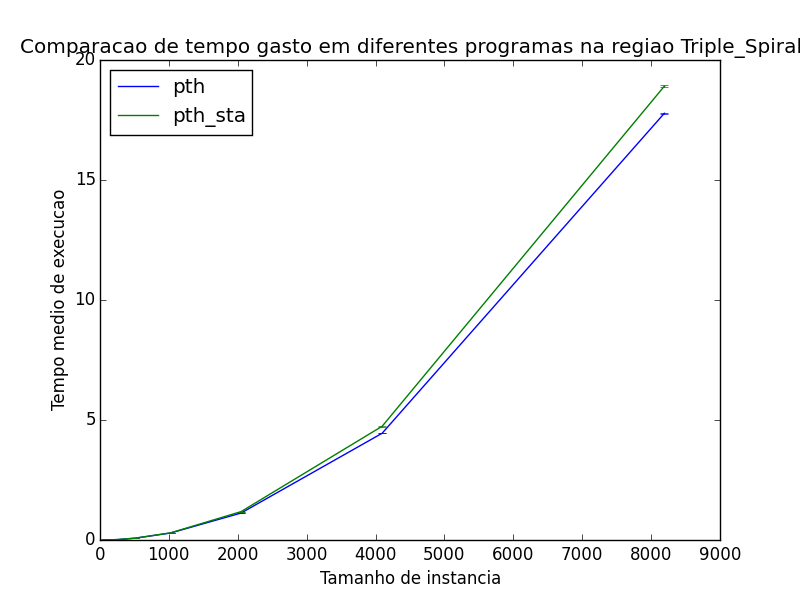
\includegraphics{pthread_din_sta/time_x_sizepth-pth_statriple_spiral.png}}
            \label {fig:pthreads_din_sta:C}
        }
        &
        \subfigure[] {\scalebox{.35}{
            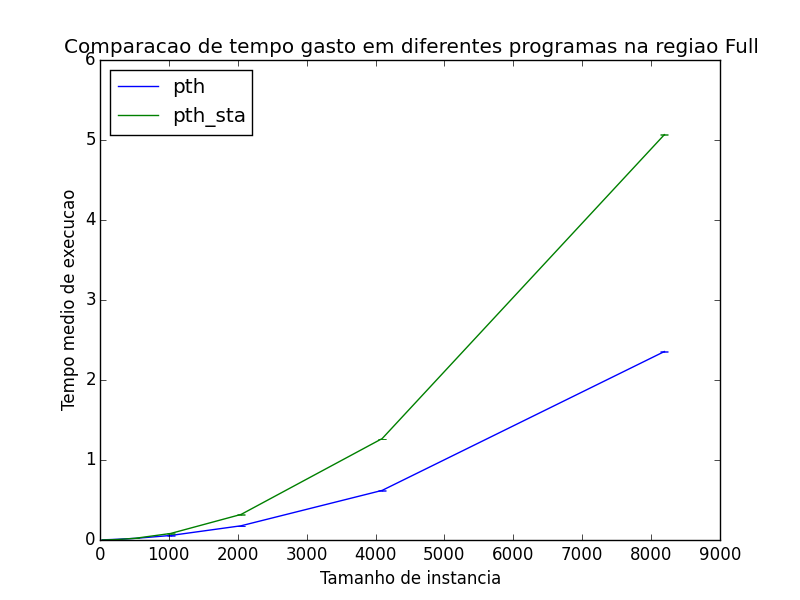
\includegraphics{pthread_din_sta/time_x_sizepth-pth_stafull.png}}
            \label {fig:pthreads_din_sta:D}
        }
        
    \end{tabular}
    \caption{Podemos observar nessas figuras que a implementação com
    divisão dinâmica possui desempenho melhor do que estático e que, 
    além disso, essa diferença tende a aumentar quando o tamanho da
    instância também aumenta. É provavel que as regiões onde o trabalho
    está 
    Esses testes foram realizados com número de threads igual
    a quantidade de processadores da máquina.}
    \label{fig:pthreads_din_sta} 
\end{figure}

Mas o que acontece quando rodamos a versão estática com muitas threads
e comparamos com a versão dinâmica? Para responder essa dúvida, 
decidimos comparar as duas implementações em pthreads de maneira que o
número de {\em chunks} fosse igual em ambas. Para o código dinâmico, o
número de threads se manteve igual ao número de cores da máquina 
enquanto que para o código estático o número de threads passou a ser
igual a quantidade de pixels em uma linha da imagem. Note que enquanto
a primeira estratégia cuida do escalonamento dos chunks para cada 
thread, a segunda cria uma thread para cada chunk e joga a 
responsabilidade para baixo, com o sistema operacional.

O que observamos nesse experimento, apresentado na 
\ref{fig:pthreads_din_sta2}, é que o desempenho de ambas estratégias foi
muito parecido, com desempenho melhor do código estático em instâncias
de tamanho perto de $2^{13}$. O motivo da implementação dinâmica ter 
desempenho pior se deve provavelmente ao nosso escalonador em pthreads,
que precisa criar e dar join em threads várias vezes. Poderíamos fazer
outra implementação onde a própria thread "escolhe" um chunk para 
calcular, mas não o faremos por falta de tempo. Apesar disso, é visível
que esse overhead se torna insignificante conforme aumentamos o tamanho
da instância sendo resolvida. 

Por fim, consideramos melhor a implementação dinâmica, porque ela 
depende menos do sistema operacional e máquina utilizada. Muitos 
sistemas operacionais definem limite na quantidade de processos na 
máquina, o que traz um limite no programa estático. Além disso, caso o 
escalonador do sistema usado seja muito ruim, o desempenho do código 
dinâmico deve ser muito melhor.


\begin{figure}[!h]
    \centering
    \begin{tabular}{c c}
        \subfigure[] {\scalebox{.35}{
            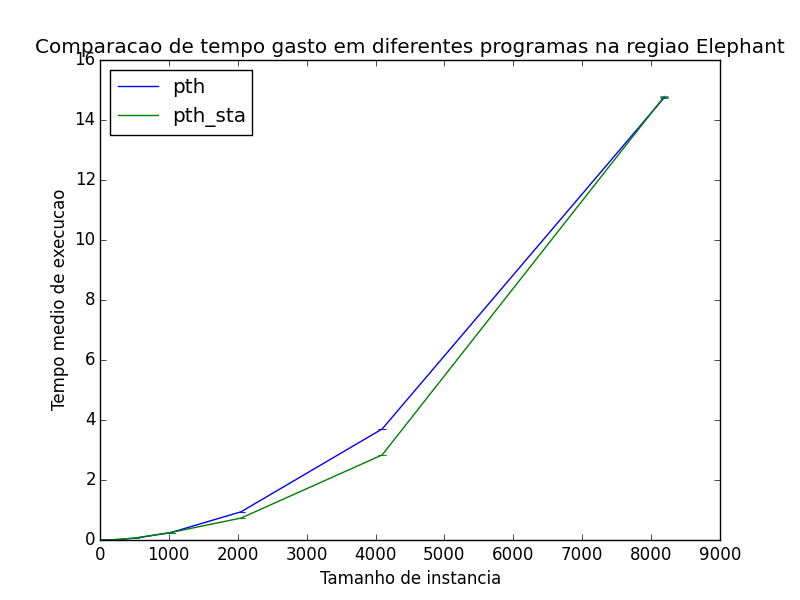
\includegraphics{pthread_din_sta/time_x_sizepth-pth_staelephant2.png}}
            \label {fig:pthreads_din_sta2:A}
        }
        &
        \subfigure[] {\scalebox{.35}{
        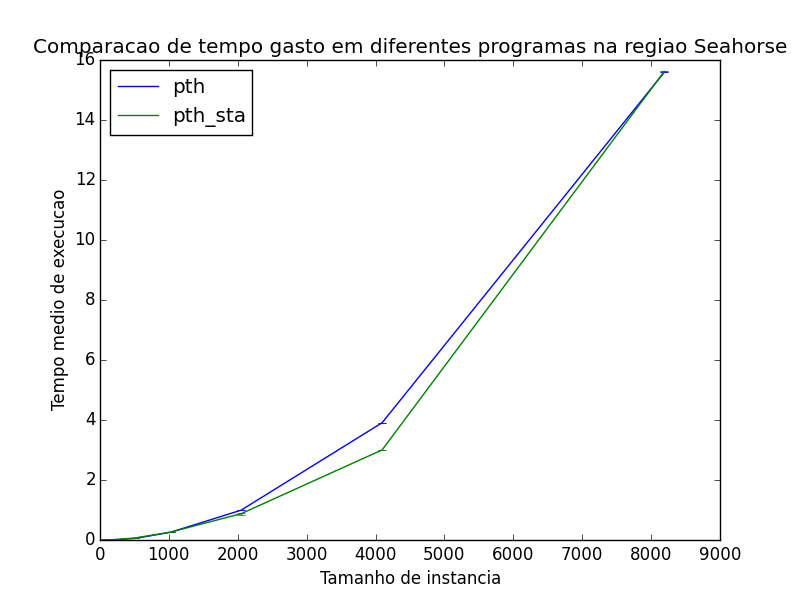
\includegraphics{pthread_din_sta/time_x_sizepth-pth_staseahorse2.png}
        }
            \label {fig:pthreads_din_sta2:B}
        }
        \\
        \subfigure[] {\scalebox{.35}{
            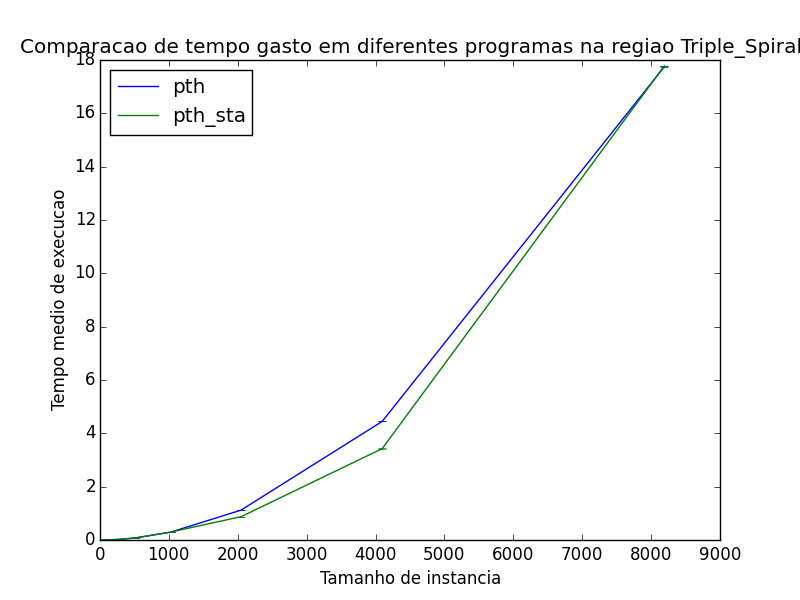
\includegraphics{pthread_din_sta/time_x_sizepth-pth_statriple_spiral2.png}}
            \label {fig:pthreads_din_sta2:C}
        }
        &
        \subfigure[] {\scalebox{.35}{
            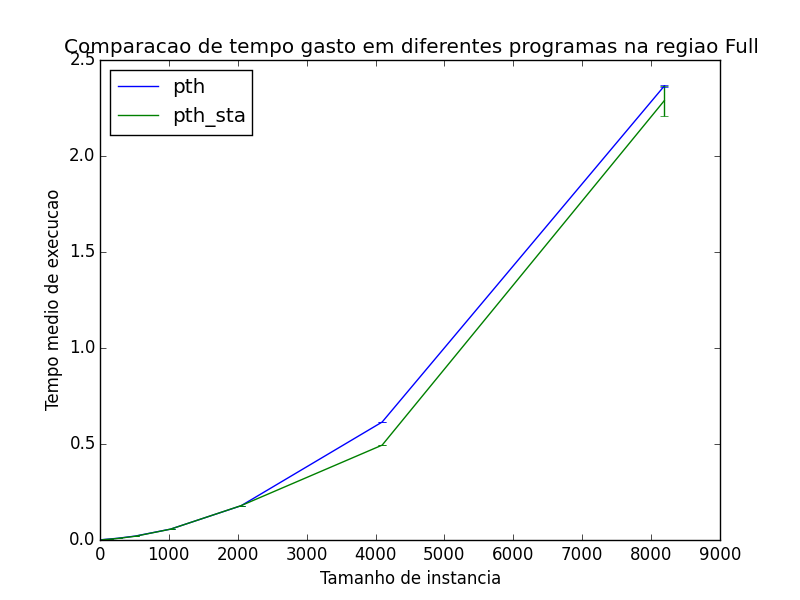
\includegraphics{pthread_din_sta/time_x_sizepth-pth_stafull2.png}}
            \label {fig:pthreads_din_sta2:D}
        }
        
    \end{tabular}
    \caption{Neste teste, o número de threads usada na implementação 
    estática foi igual ao de pixels em uma linha da imagem.
    No código dinâmico, o número de threads foi exatamente o número de 
    processadores da máquina, além disso, a quantidade de chunks é
    igual ao número de pixels em uma linha da imagem. Lembrando que o
    código estático cria um número de chunks igual ao de threads,
    podemos dizer que o número de chunks é igual em ambas 
    implementações.
    }
    \label{fig:pthreads_din_sta2} 
\end{figure}


%%%%%%%%%%%%%%%%%%%%% OPENMP %%%%%%%%%%%%%%%%%%%%%%%%%%%%%%
\newpage
\section{Código em OpenMP}
Para implementar a versão OpenMP do programa do cálculo do conjunto de 
Mandelbrot tivemos que remover a alocação de memória e comandos de 
leitura e escrita do código fornecido previamente. Como não há comandos
de leitura, os comandos de leitura e escrita são retirados, removendo-se
a função \code{write\_to\_file()}. No caso de alocação de memória pode 
ser que o tempo de acesso a um vetor possa ser relevante, portanto não
simplesmente removemos a função de alocação de memória. Para retirar as
alocações, supomos que o tamanho máximo de uma imagem será de 11500px x
11500px e assim substituímos a alocação dinâmica do \code{image\_buffer}
por uma alocação estática: \code{char image\_buffer[11500*11500][3]}.

Para paralelizar o cálculo, como esperado do OpenMP, é tão fácil como
adicionar um \code{\#pragma} antes do \code{for} que realiza o cálculo
para cada pixel da imagem:
\begin{lstlisting}[style=CStyle]
    #pragma omp parallel for private(...) num_threads(nThreads) schedule(dynamic)
    for (i_y = 0; i_y < i_y_max; i_y++) {
        c_y = c_y_min + i_y * pixel_height;
        ...
\end{lstlisting}

Implementando dessa forma obtemos os seguintes resultados:
\begin{figure}[H]
    \makebox[\textwidth][c]{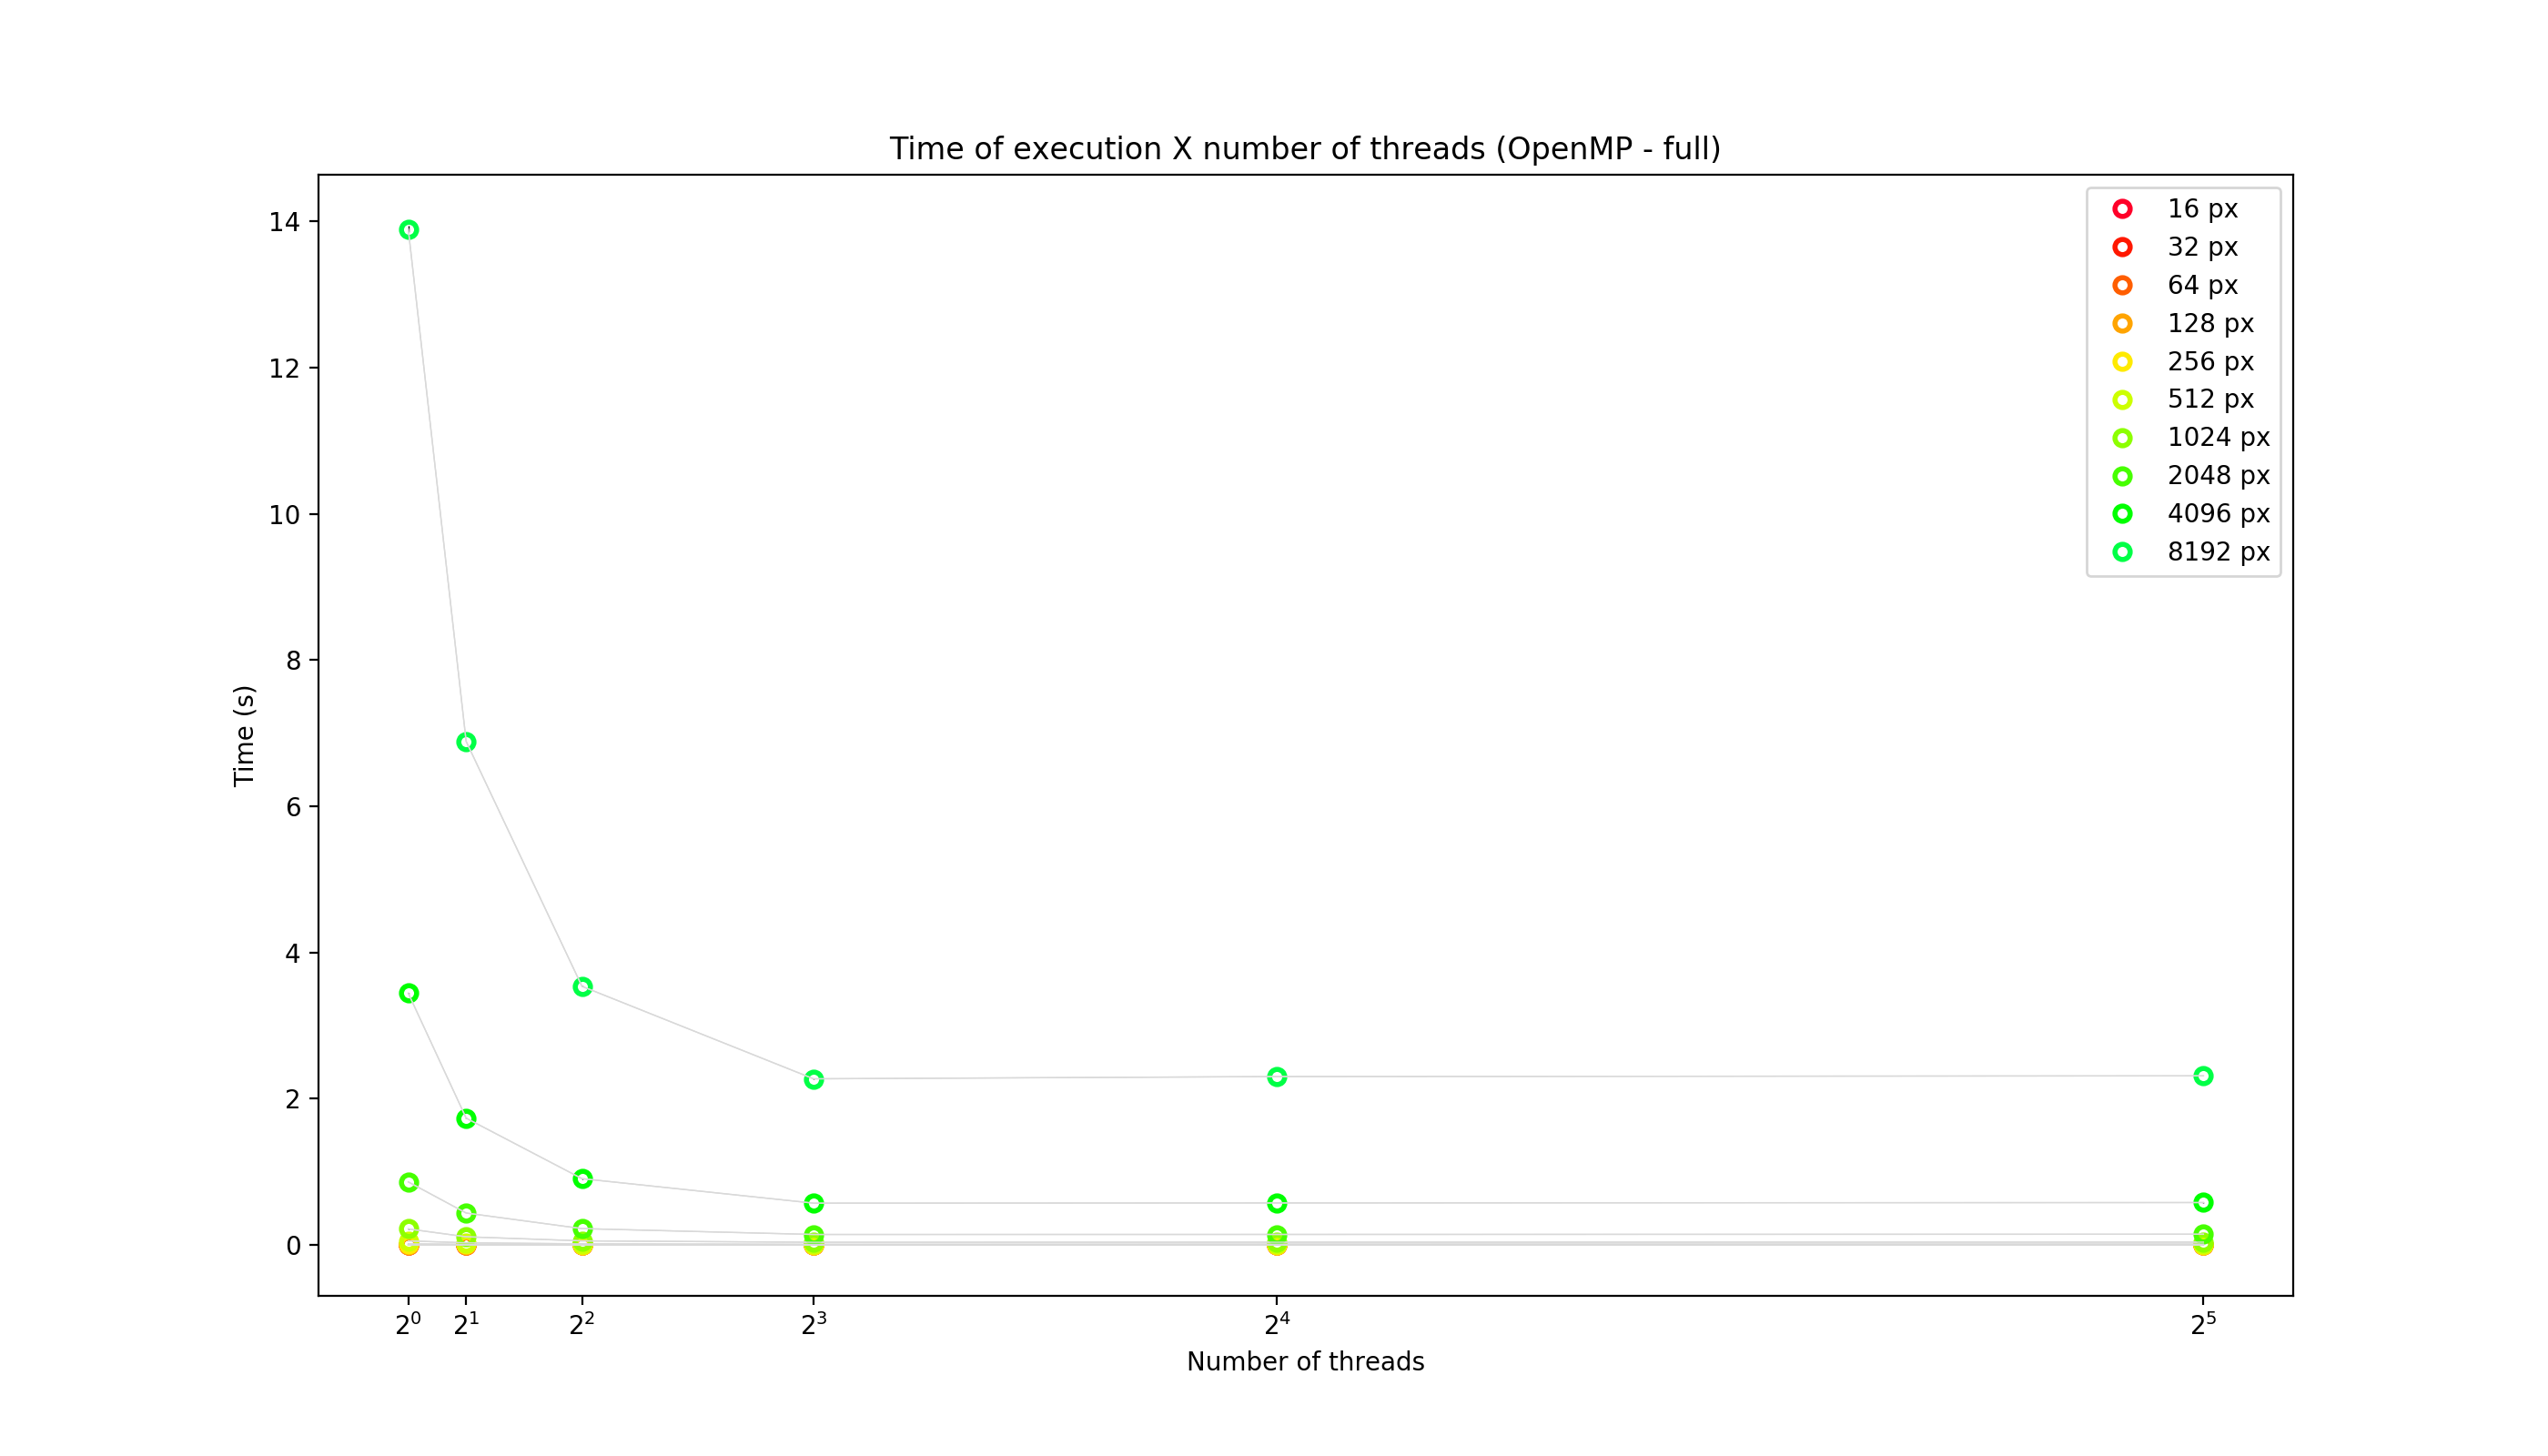
\includegraphics[scale=.60]{for_duplo_plot/timeXthread_full_OpenMPpng.png}}
    \caption{Esse gráfico mostra o tempo de execução X numero de threads para cada tamanho de entrada. Esses valores foram experimentados na região "full". Barras de erro também estão plotadas, porém são tão pequenas que talvez não estejam visíveis.}
\end{figure}

Percebemos que o aumento de threads de fato melhorou o tempo de execução do programa. No entanto ao ultrapassar 8, o mesmo número de cores da maquina testada, não houve grande melhora no tempo de execução. Esse mesmo comportamento foi observado para as demais regiões:

\begin{figure}[H]
    \makebox[\textwidth][c]{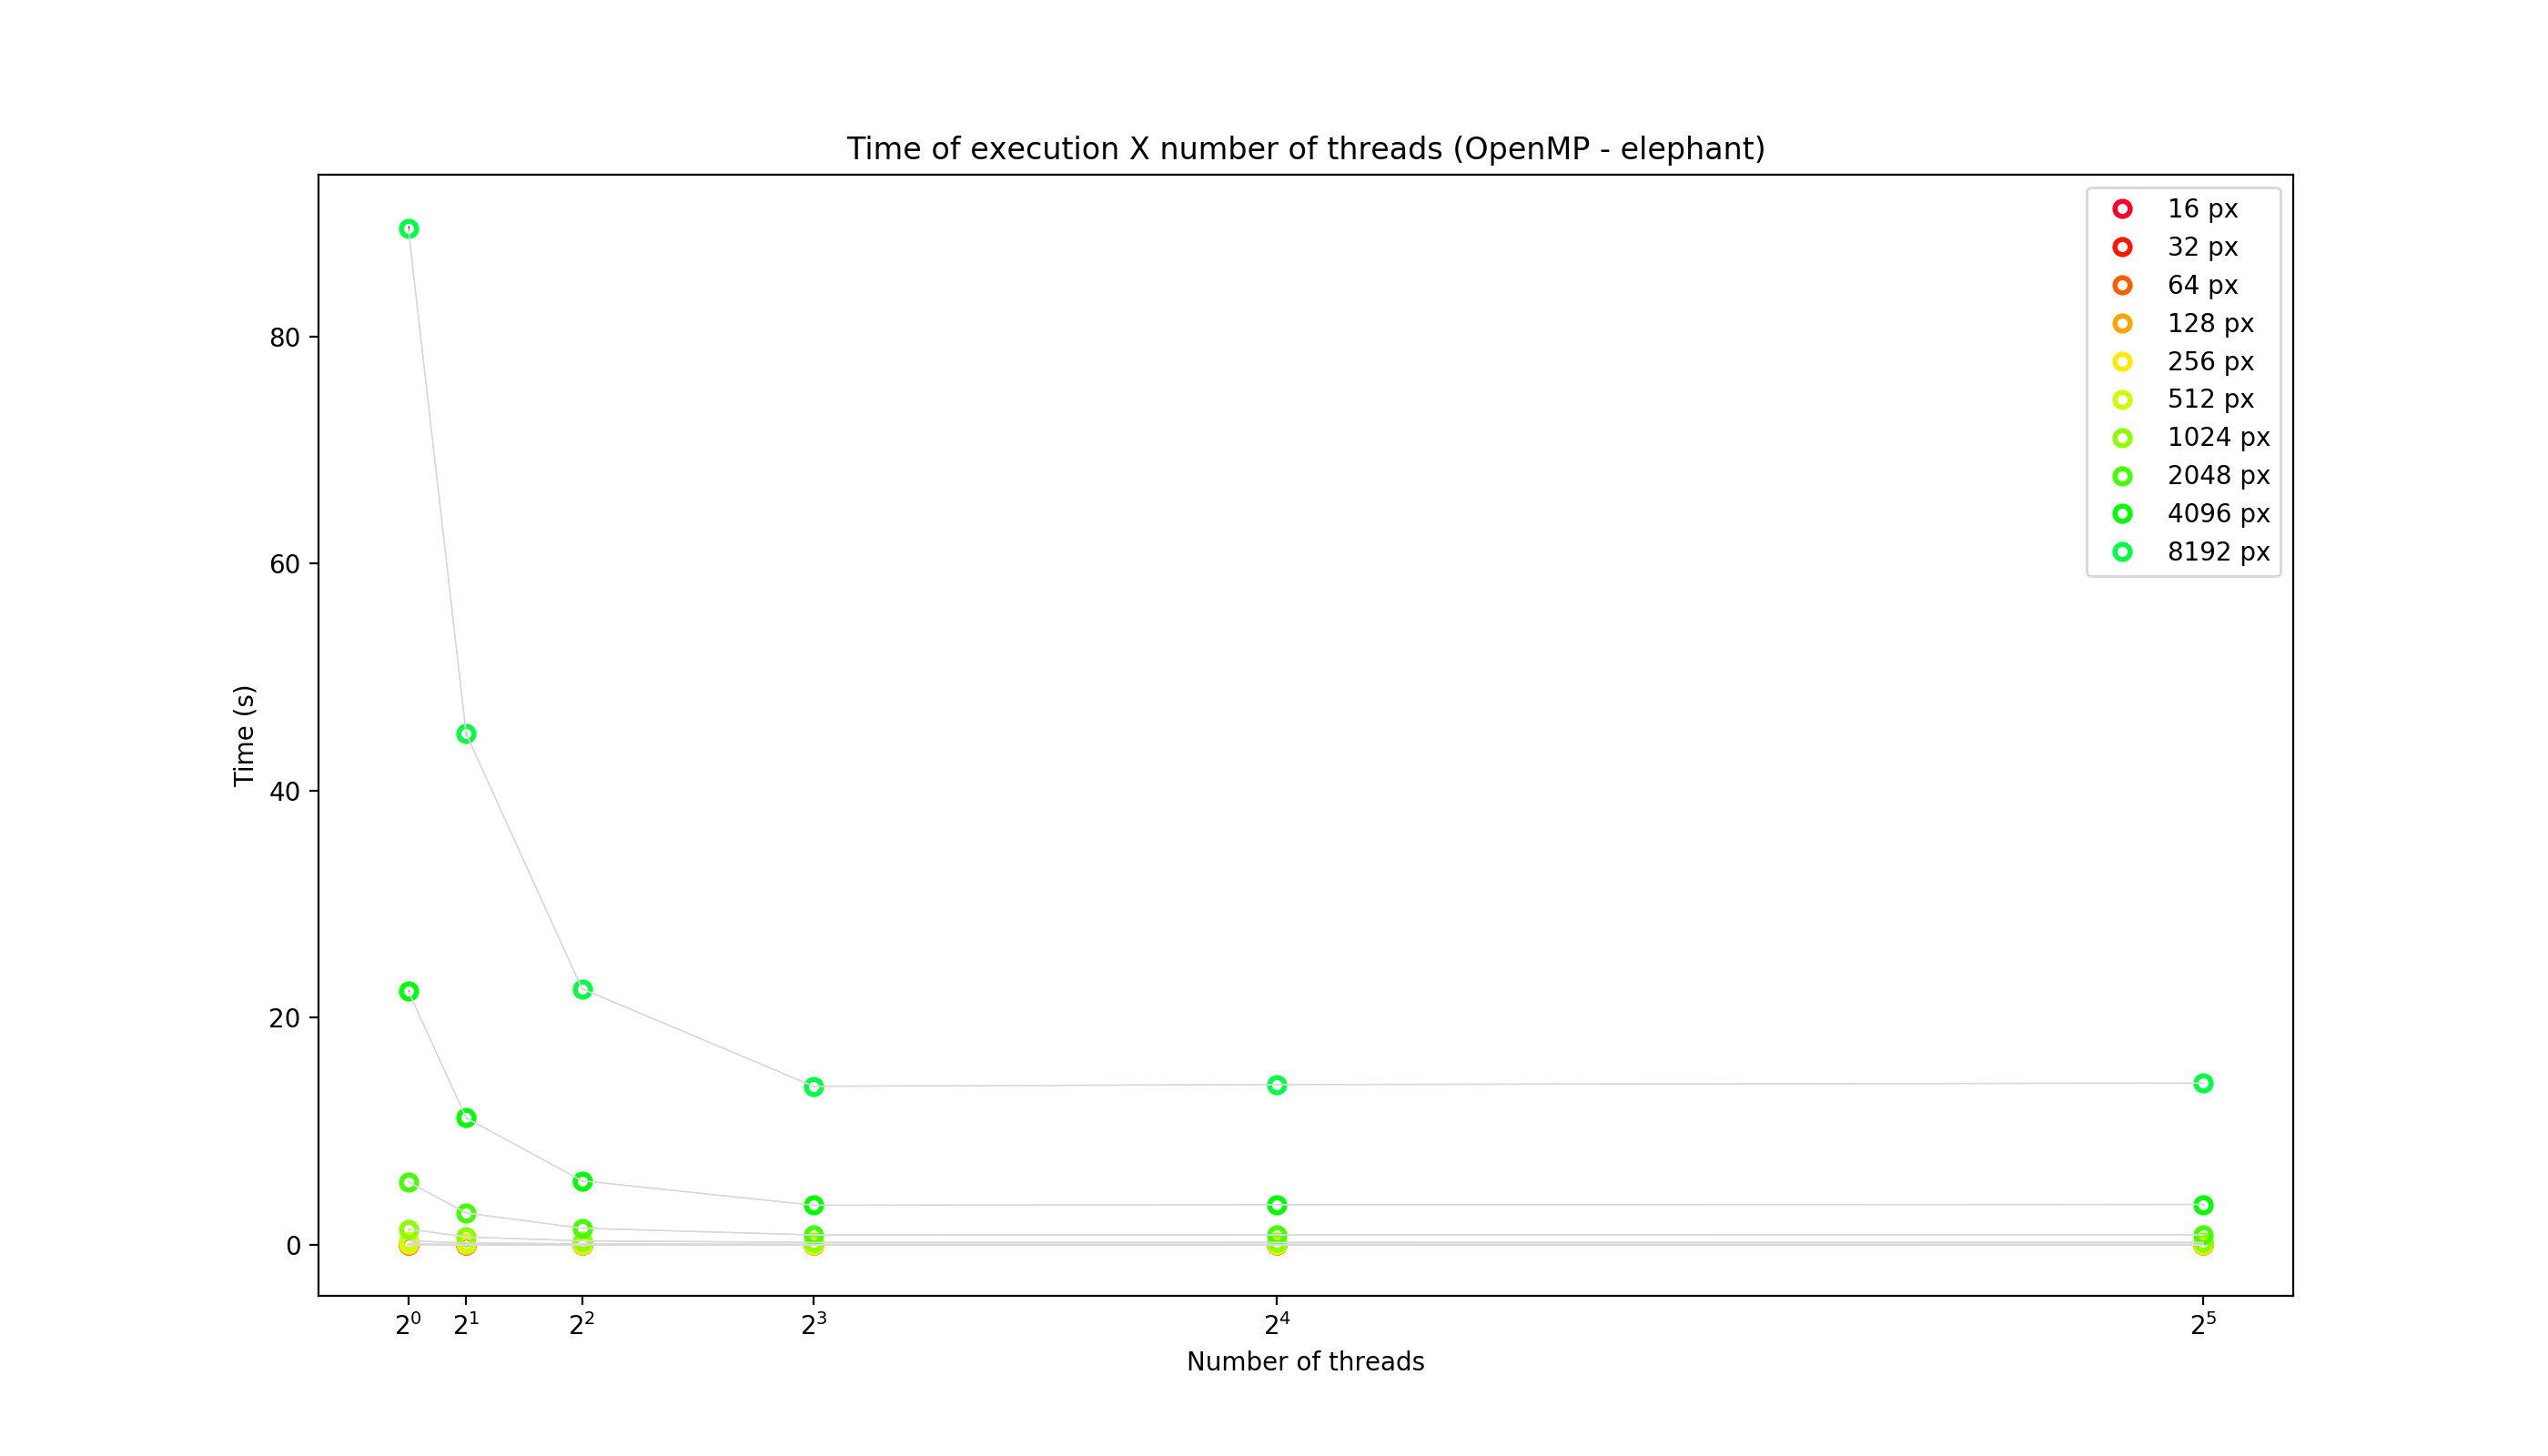
\includegraphics[scale=.50]{for_duplo_plot/timeXthread_elephant_OpenMPpng.png}}
\end{figure}

\begin{figure}[H]
    \makebox[\textwidth][c]{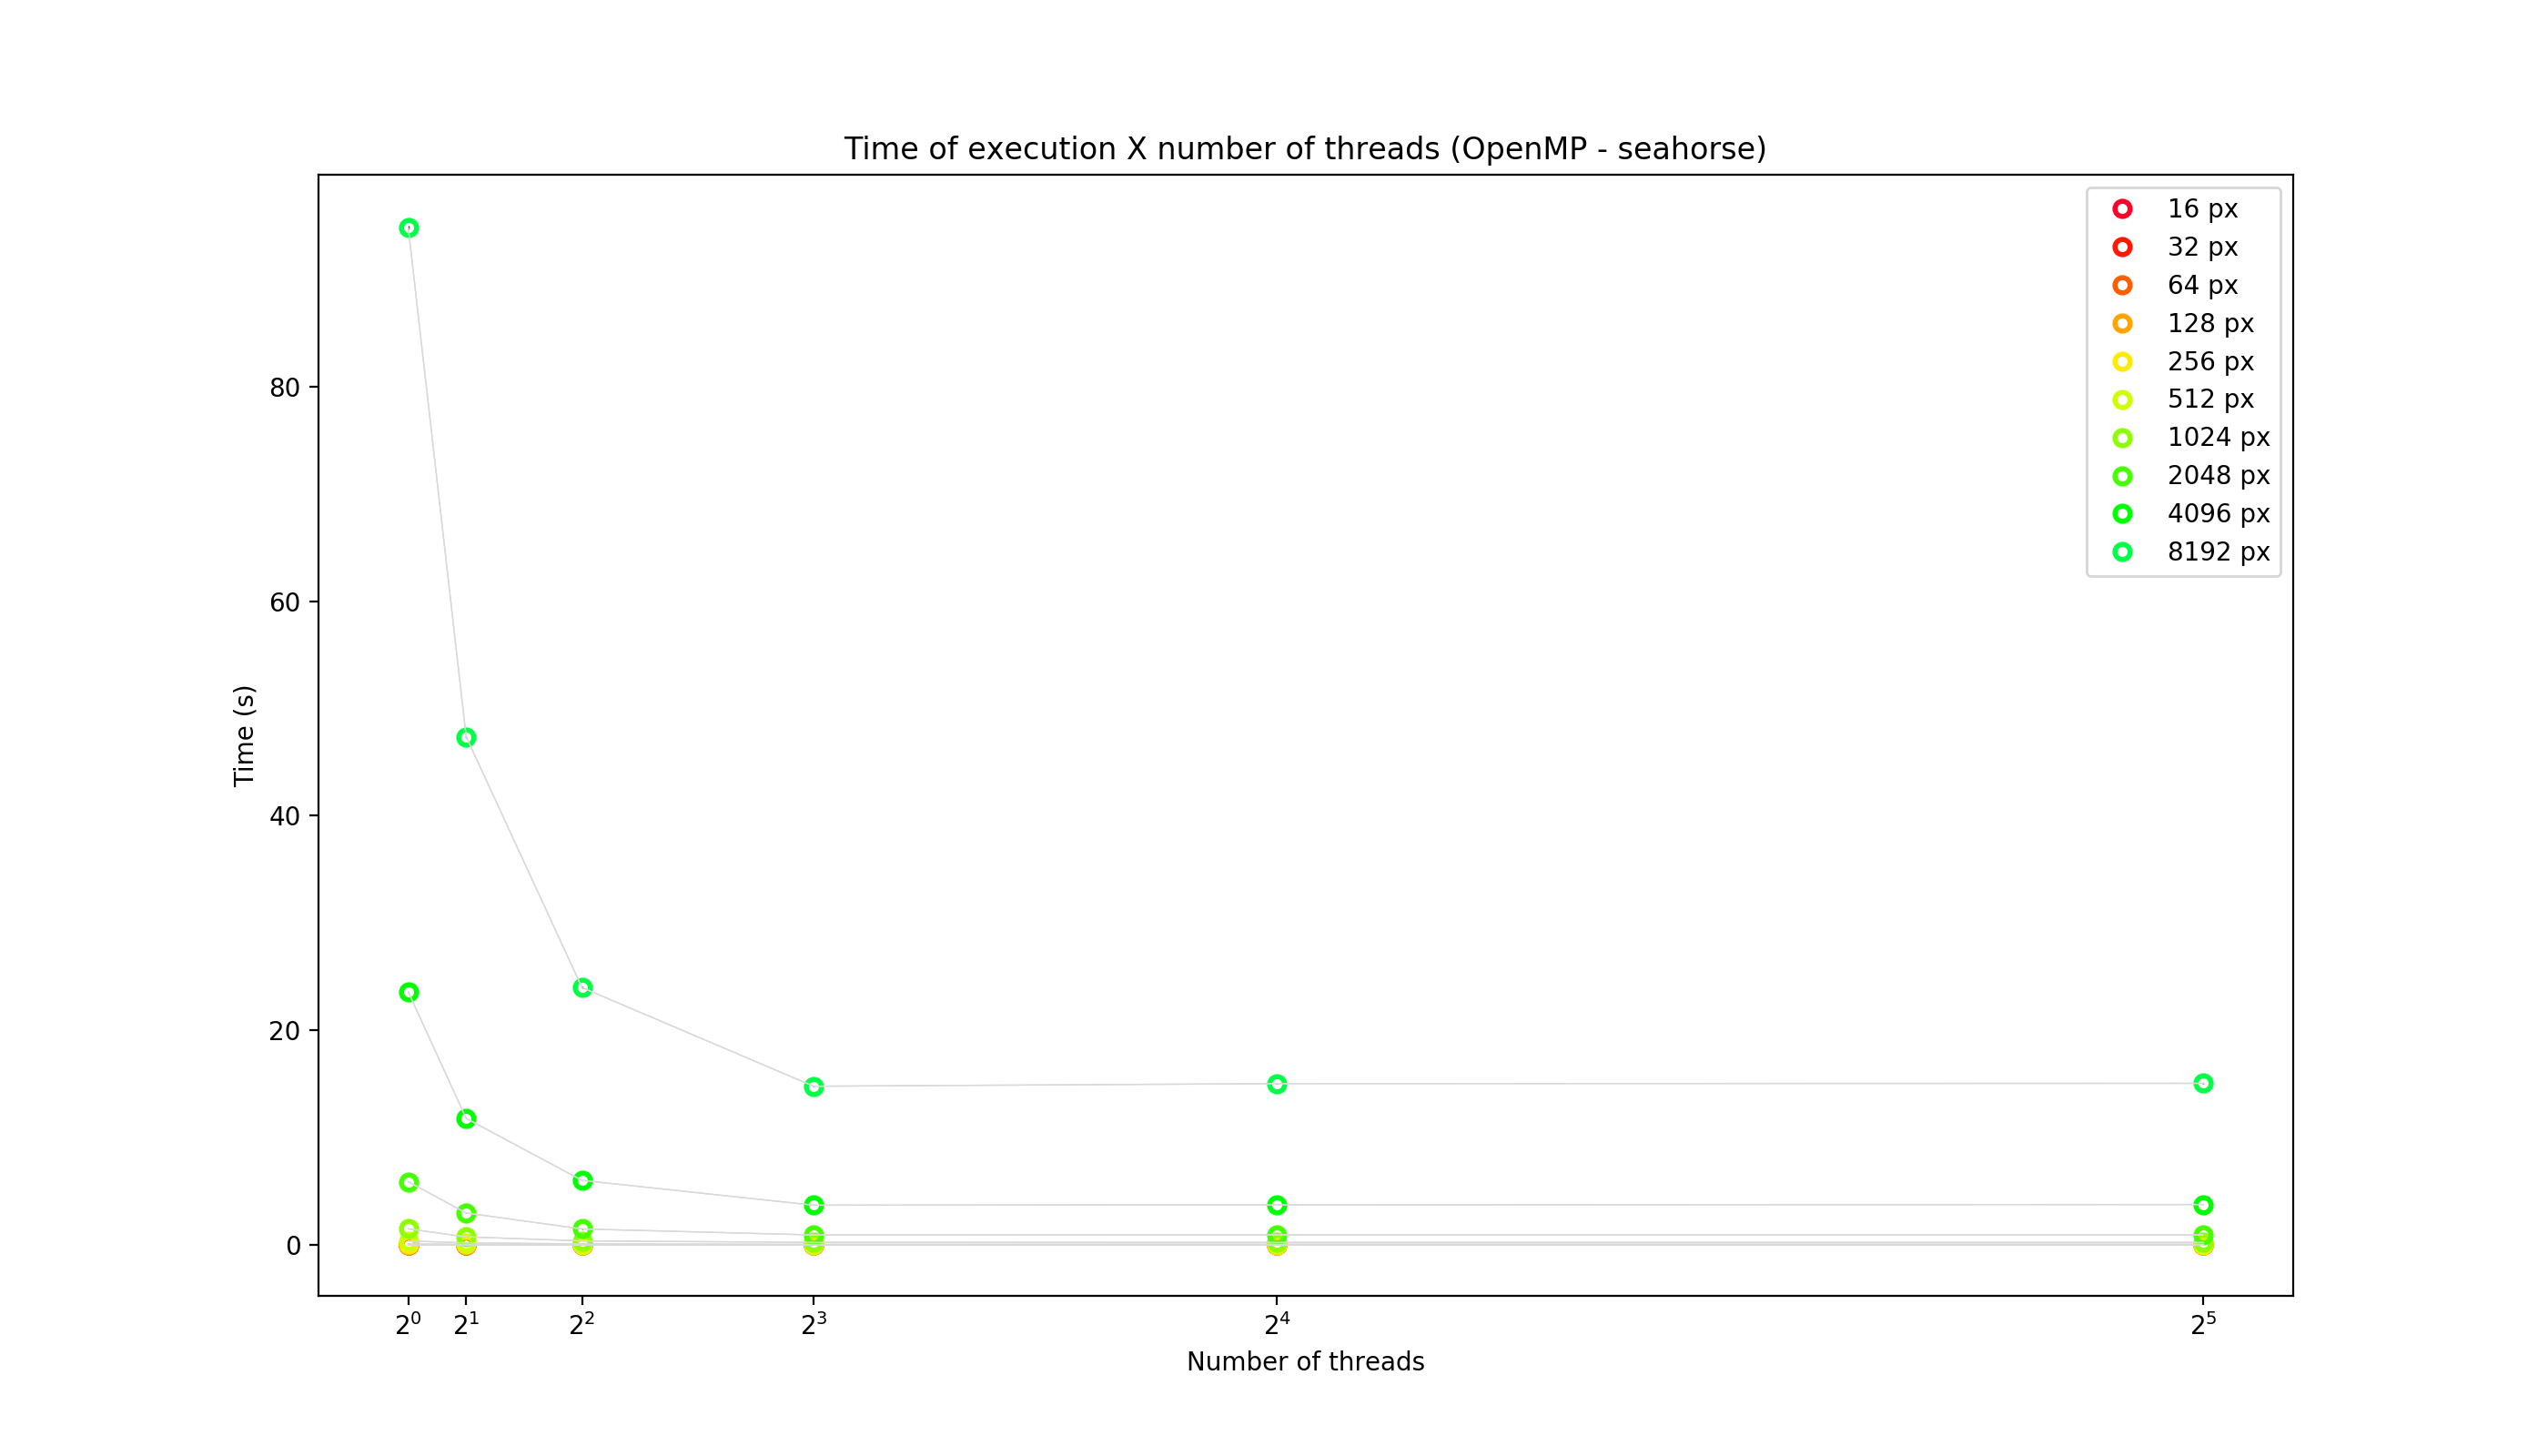
\includegraphics[scale=.50]{for_duplo_plot/timeXthread_seahorse_OpenMPpng.png}}
\end{figure}

\begin{figure}[H]
    \makebox[\textwidth][c]{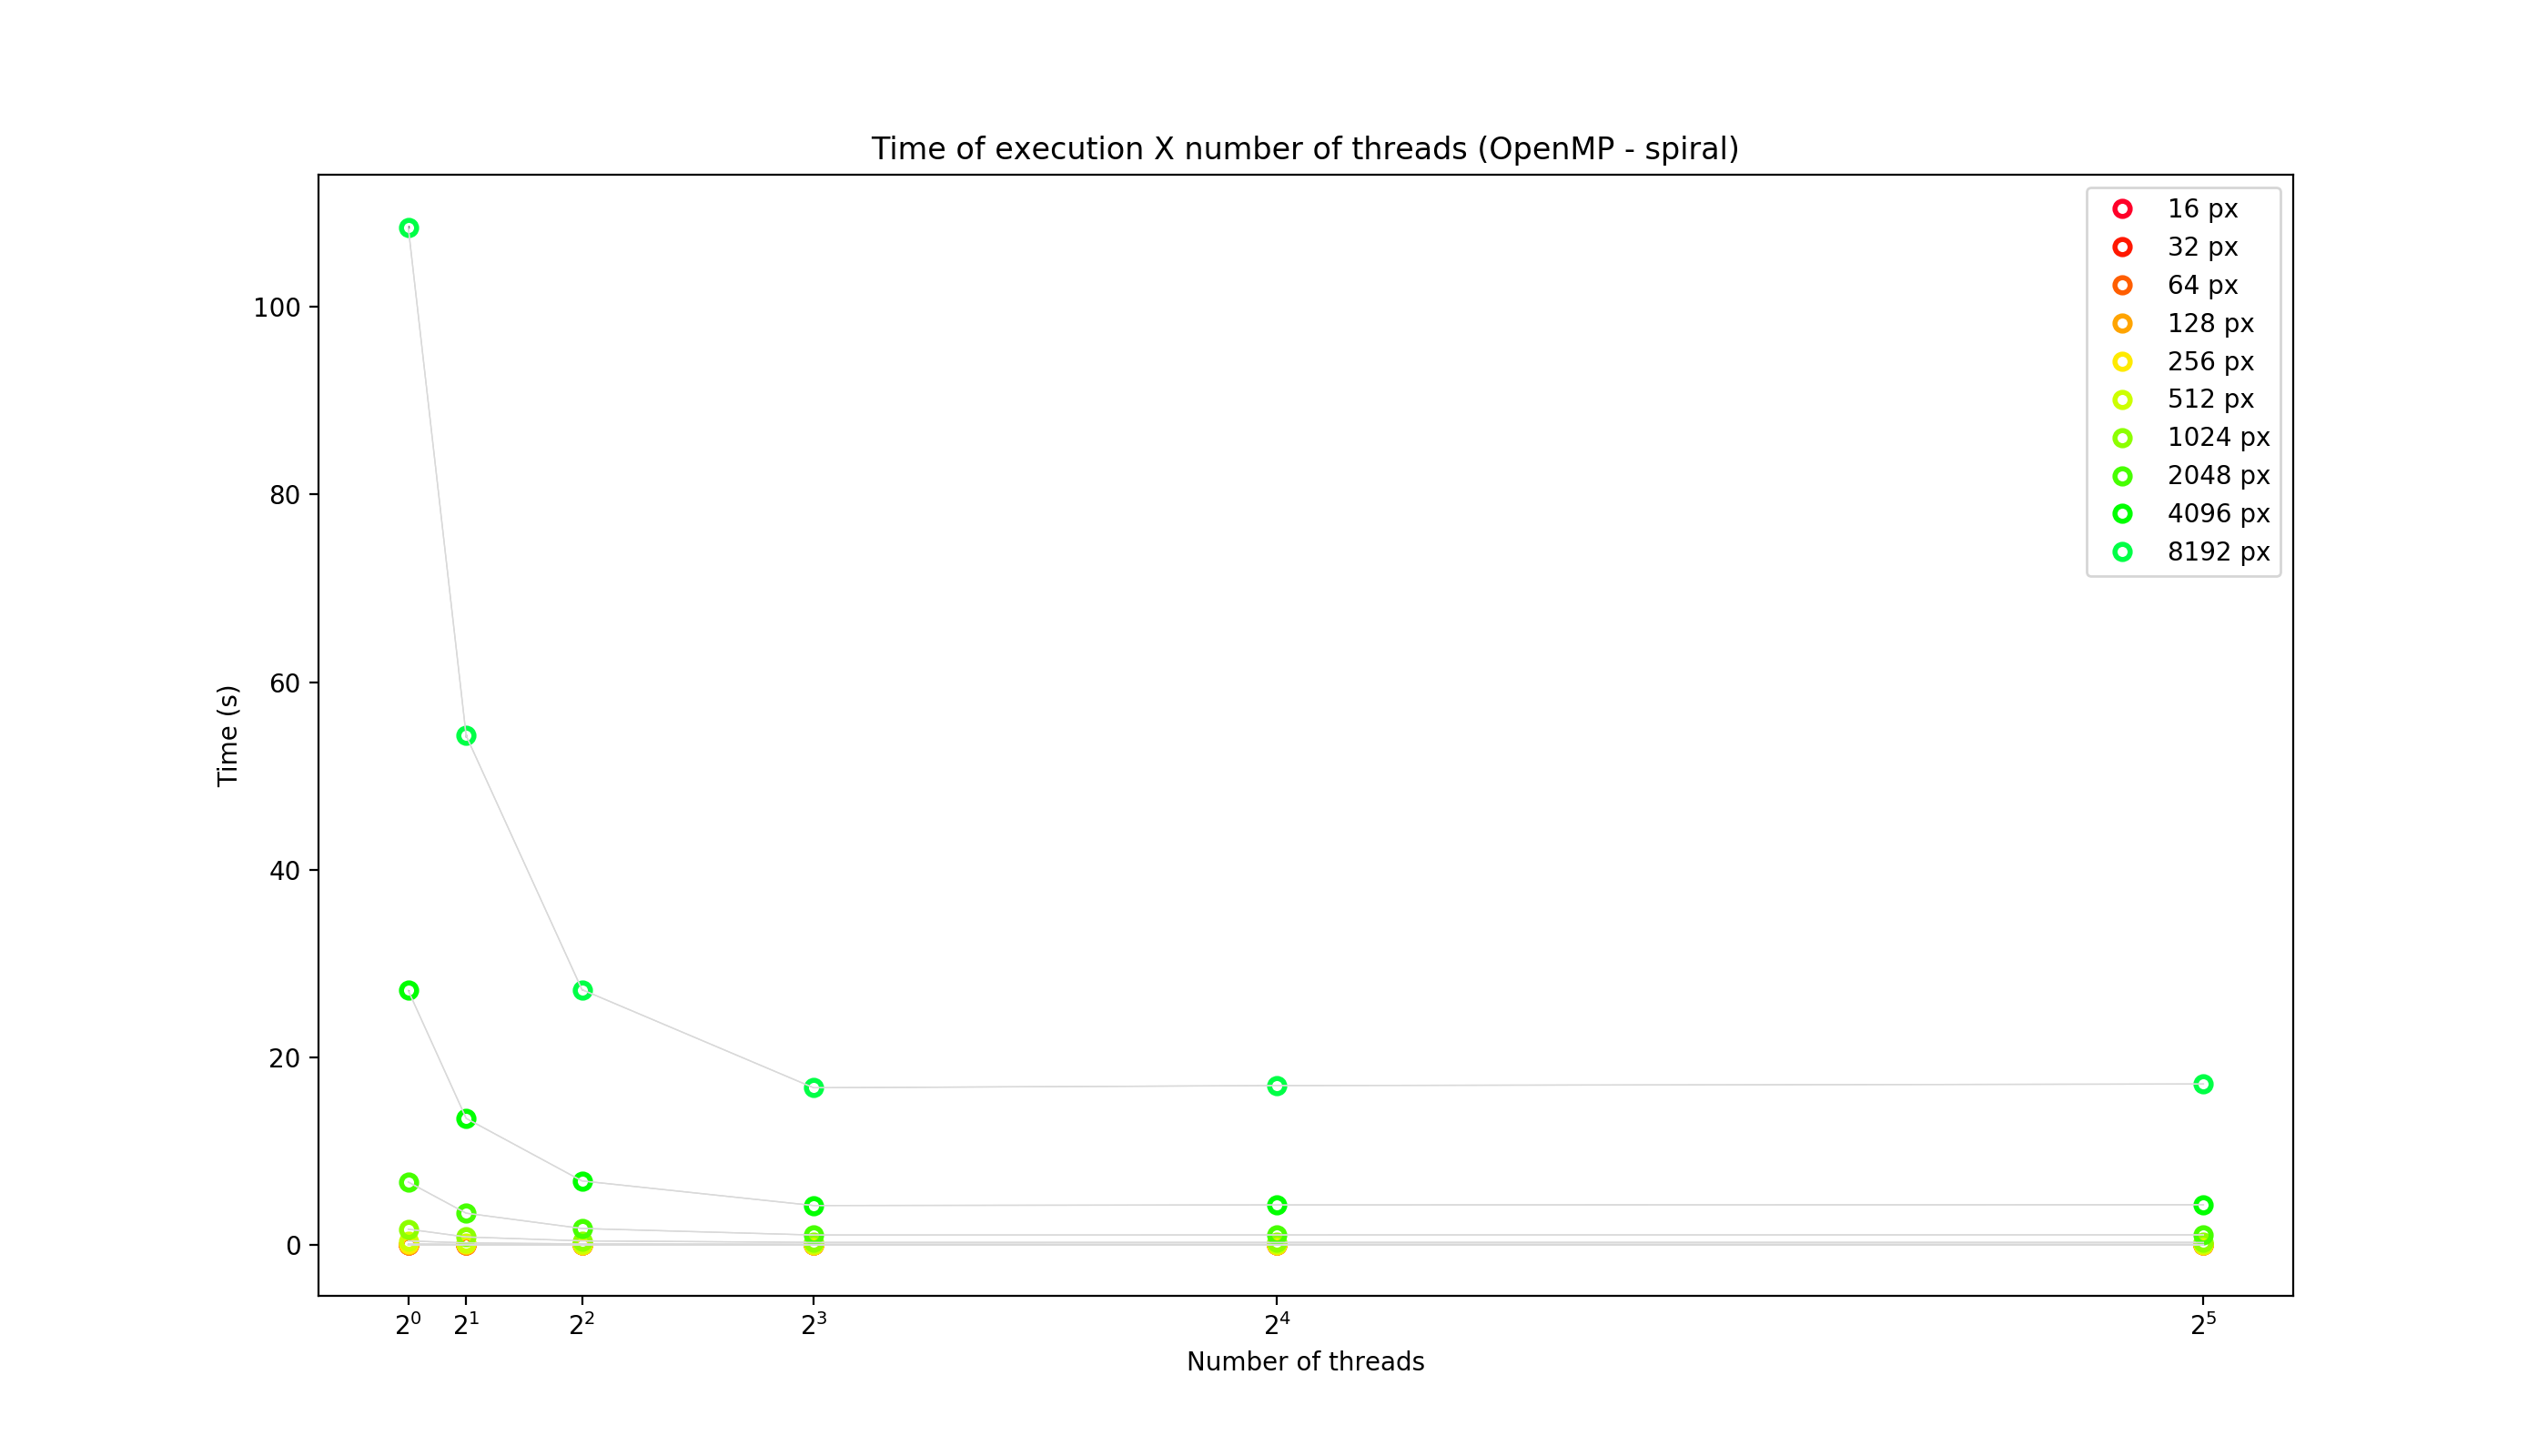
\includegraphics[scale=.50]{for_duplo_plot/timeXthread_spiral_OpenMPpng.png}}
\end{figure}

Nota-se que nessas regiões apesar do comportamento do tempo X numero de threads manter-se o mesmo, o tempo de execução aumenta, pois nessas regiões há mais cálculos de pontos com mais interações. Podemos comparar todas as regiões:

\begin{figure}[H]
    \makebox[\textwidth][c]{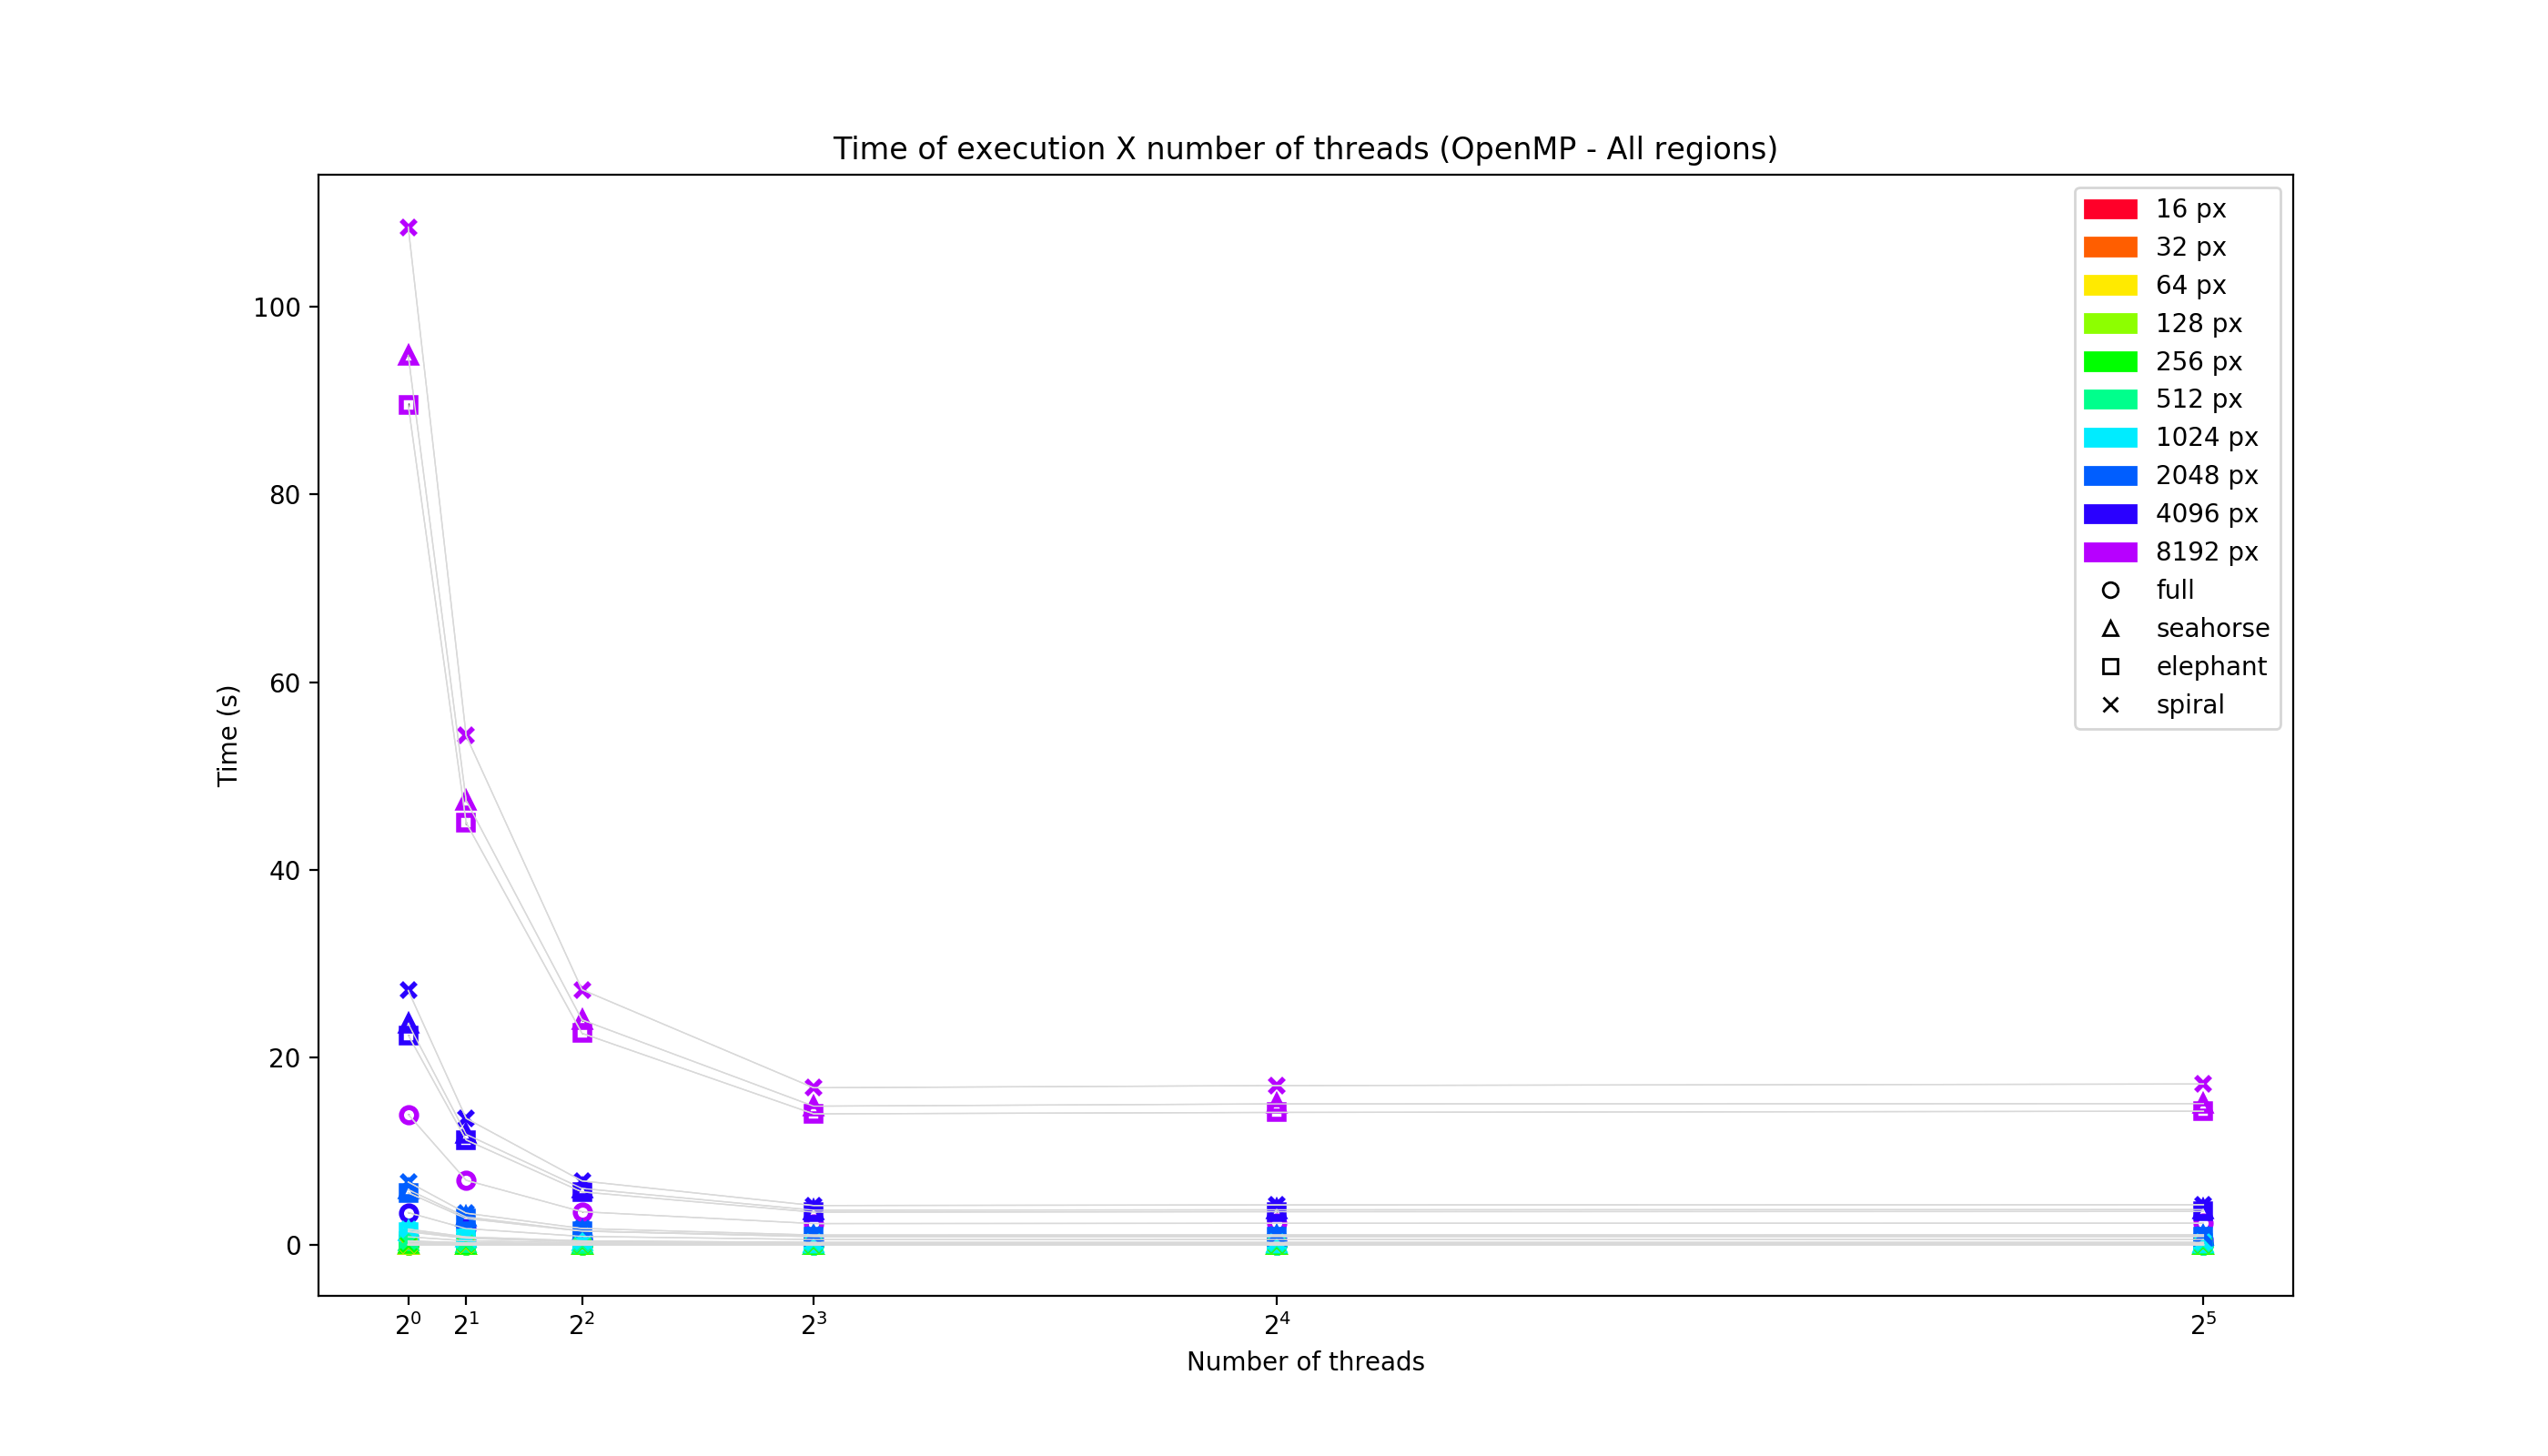
\includegraphics[scale=.50]{for_duplo_plot/all_timeXthread_OpenMPpng.png}}
\end{figure}

Vemos que as regiões Spiral, Seahorse e Elephant tem tempo de execução bastante maior que a região Full.

Em todos esses gráficos também vemos que quanto maior o tamanho da entrada, mais tempo o programa leva para ser executado. Porém também queremos saber qual é a relação entre tamanho de entrada e o tempo:

\begin{figure}[H]
    \makebox[\textwidth][c]{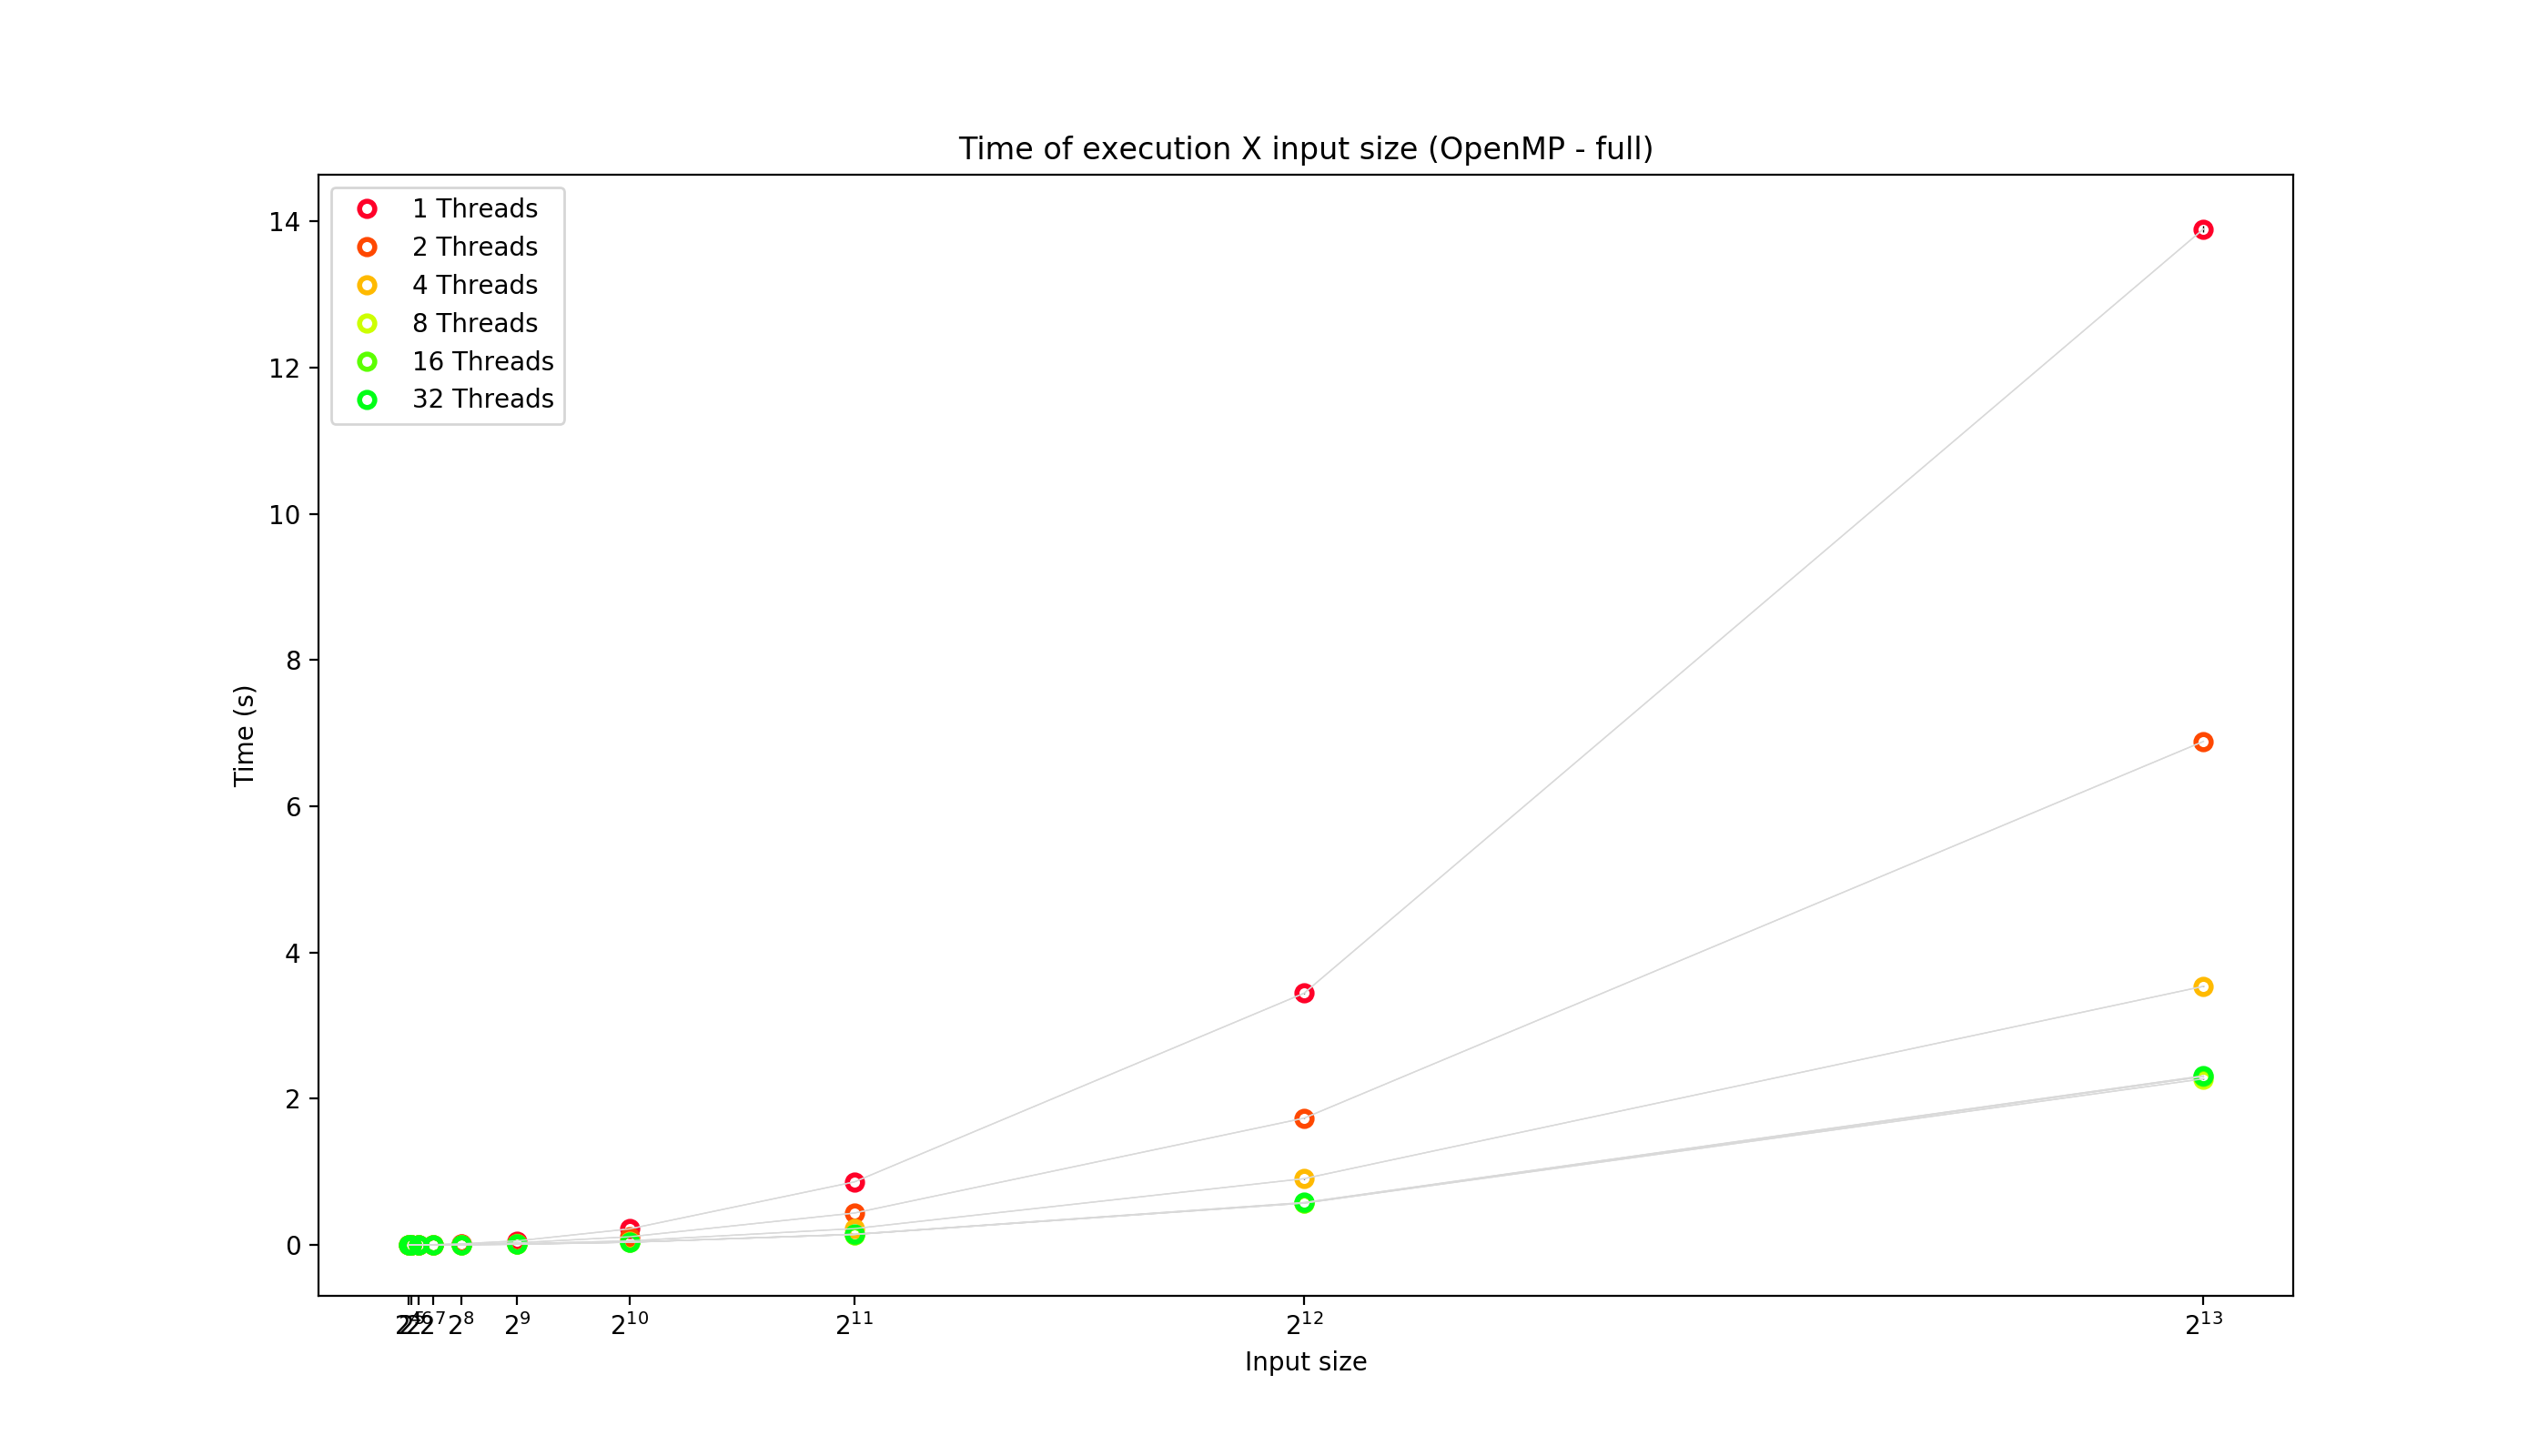
\includegraphics[scale=.50]{for_duplo_plot/timeXsize_full_OpenMPpng.png}}
\end{figure}

Vemos que há um aumento exponencial do tempo pelo tamanho da imagem. Vale lembrar que consideramos o tamanho de entrada, somente o tamanho do lado da imagem, portanto o comportamento exponencial se justifica por o número de pixels (chamadas para a função \code{compute\_manderbolt()}) ser o tamanho do lado da imagem elevado ao quadrado.

Nas demais regiões o comportamento é semelhante:

\begin{figure}[H]
    \makebox[\textwidth][c]{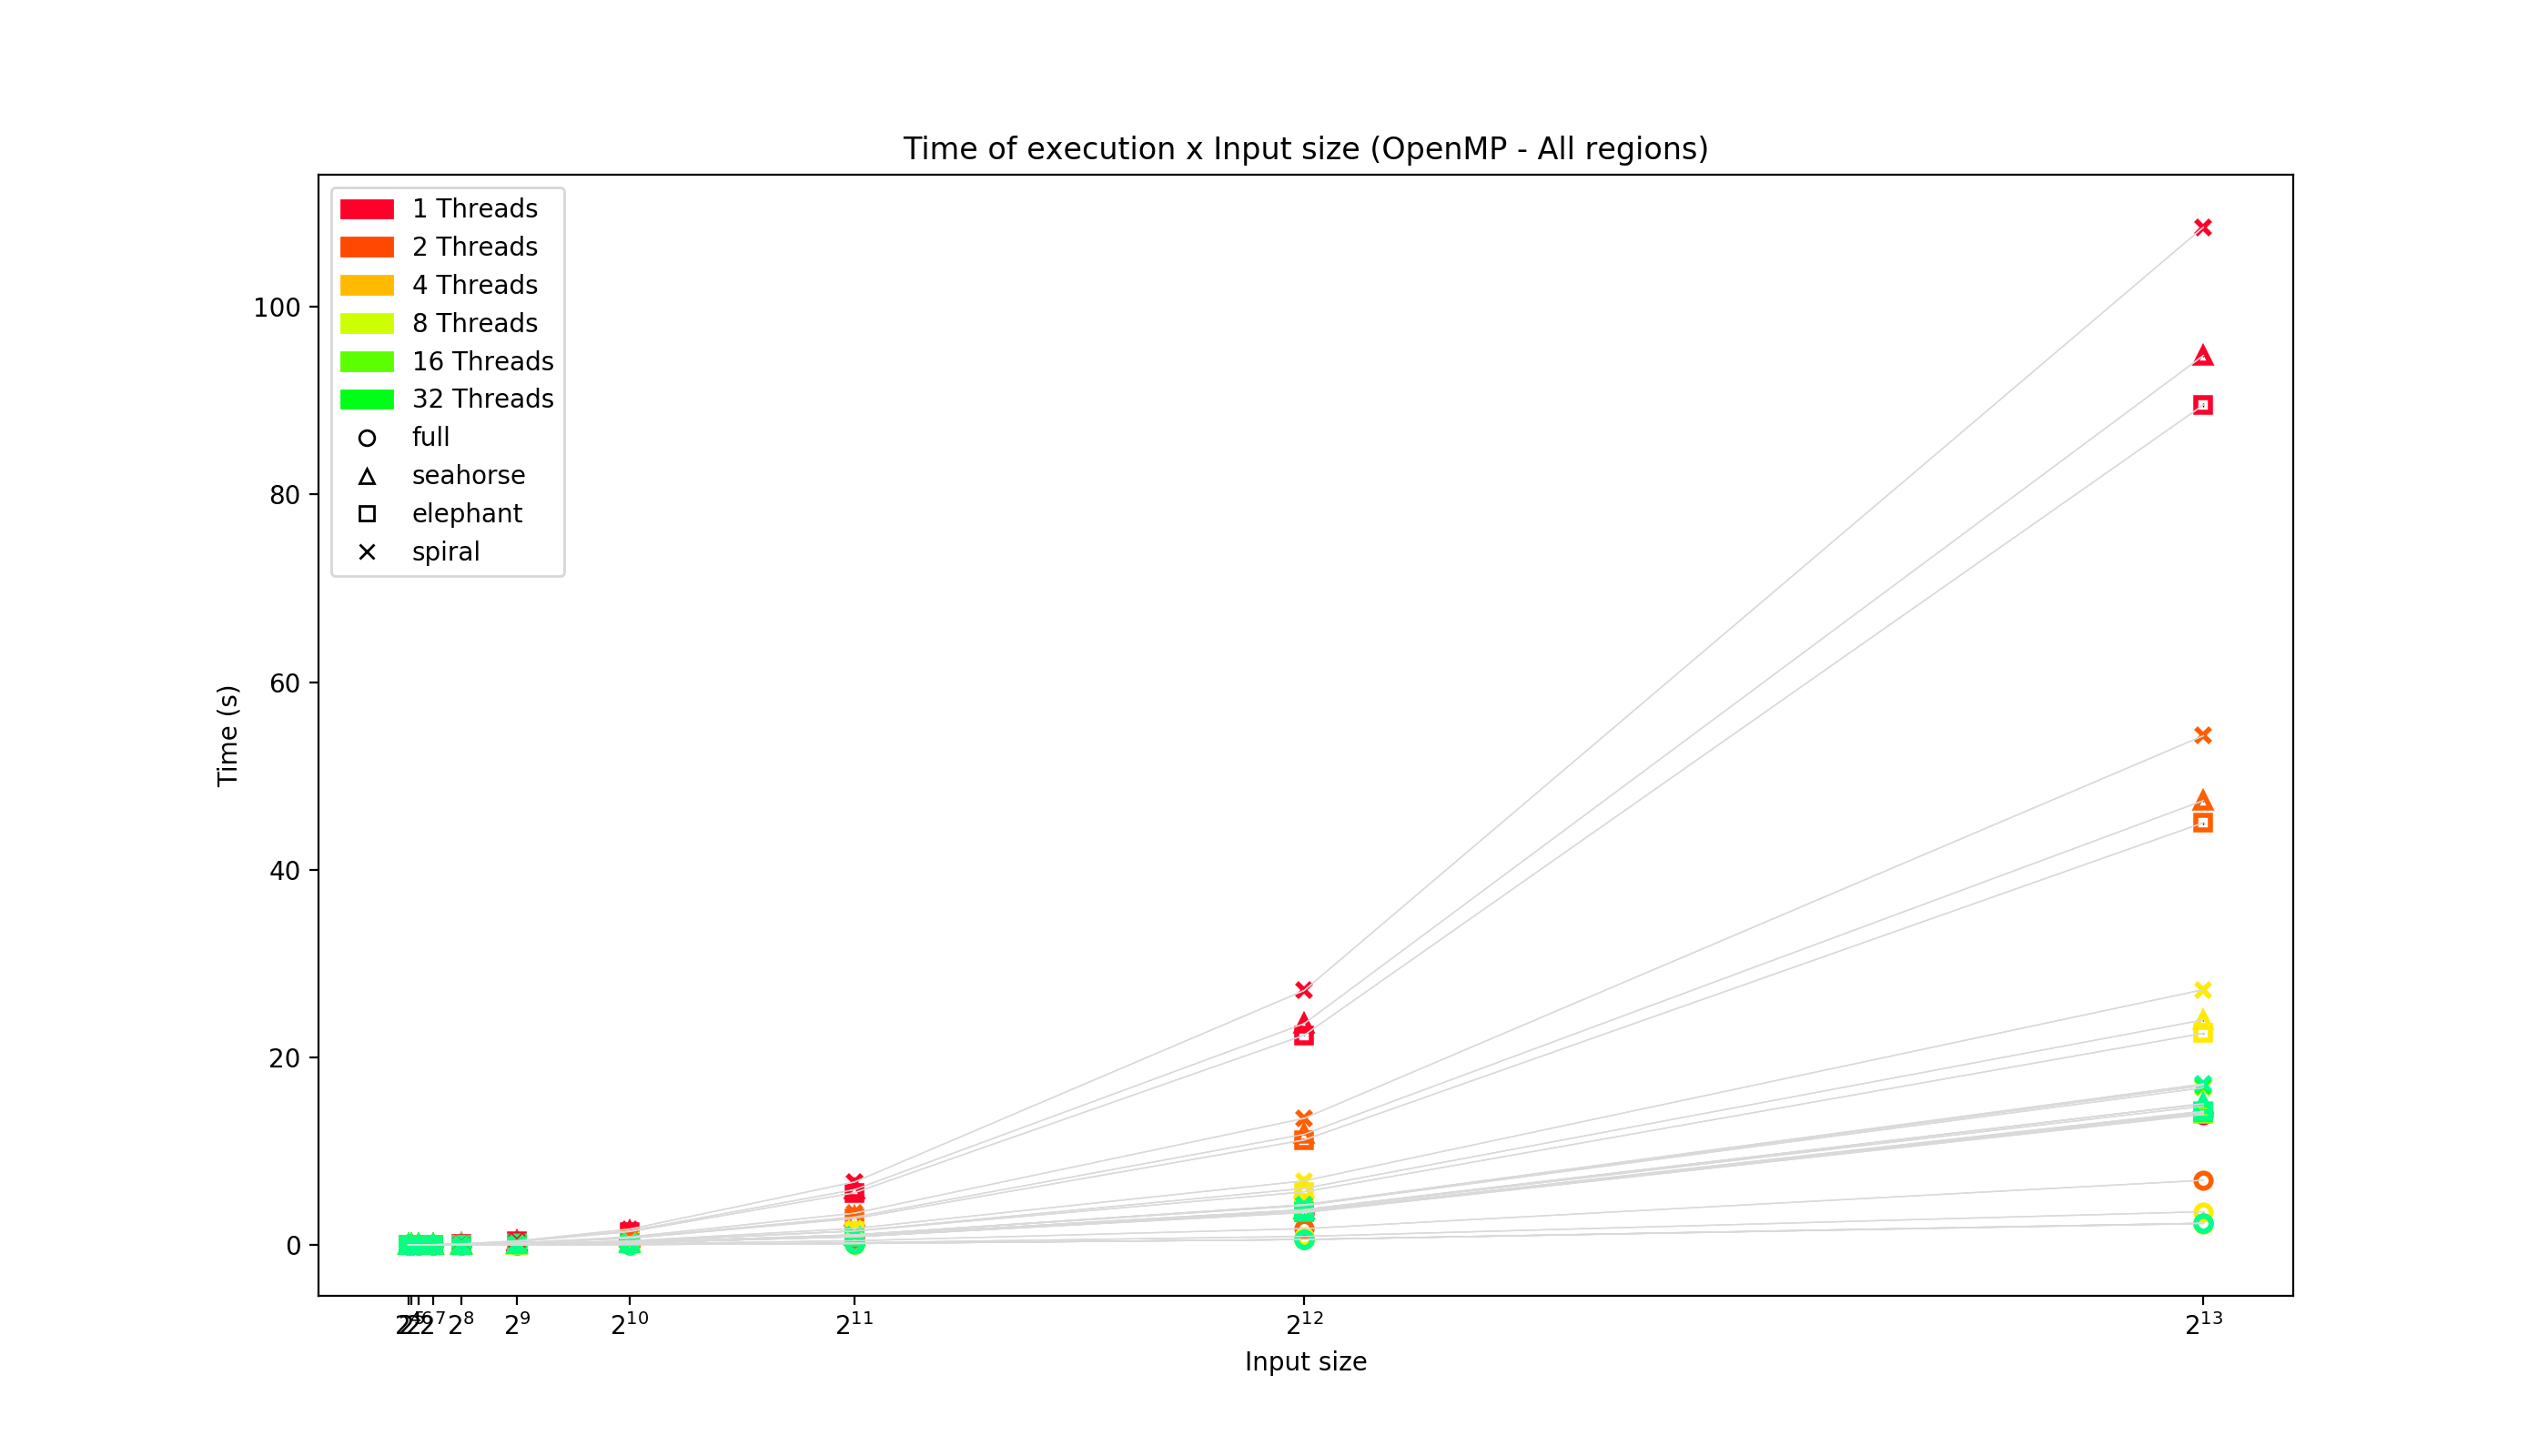
\includegraphics[scale=.50]{for_duplo_plot/all_timeXsize_OpenMPpng.png}}
\end{figure}

\subsection{Implementação com 1 for}
Após realizar esses primeiros testes imaginamos que se paralelizassemos o for de dentro o programa pudesse ficar mais rápido. Para fazer isso como eram dois fors simples, decidimos transforma-los em um só:

\begin{lstlisting}[style=CStyle]
    #pragma omp parallel for private(...) num_threads(nThreads) schedule(dynamic)
    for (i = 0; i < i_y_max * i_x_max; i++) {
        i_y = i / i_y_max;
        i_x = i % i_y_max;
        ...
\end{lstlisting}

Com essa implementação e usando \code{schedule(dynamic)}, ou seja com o chunk de tamanho 1, obtivemos os seguintes resultados:

\begin{figure}[H]
    \makebox[\textwidth][c]{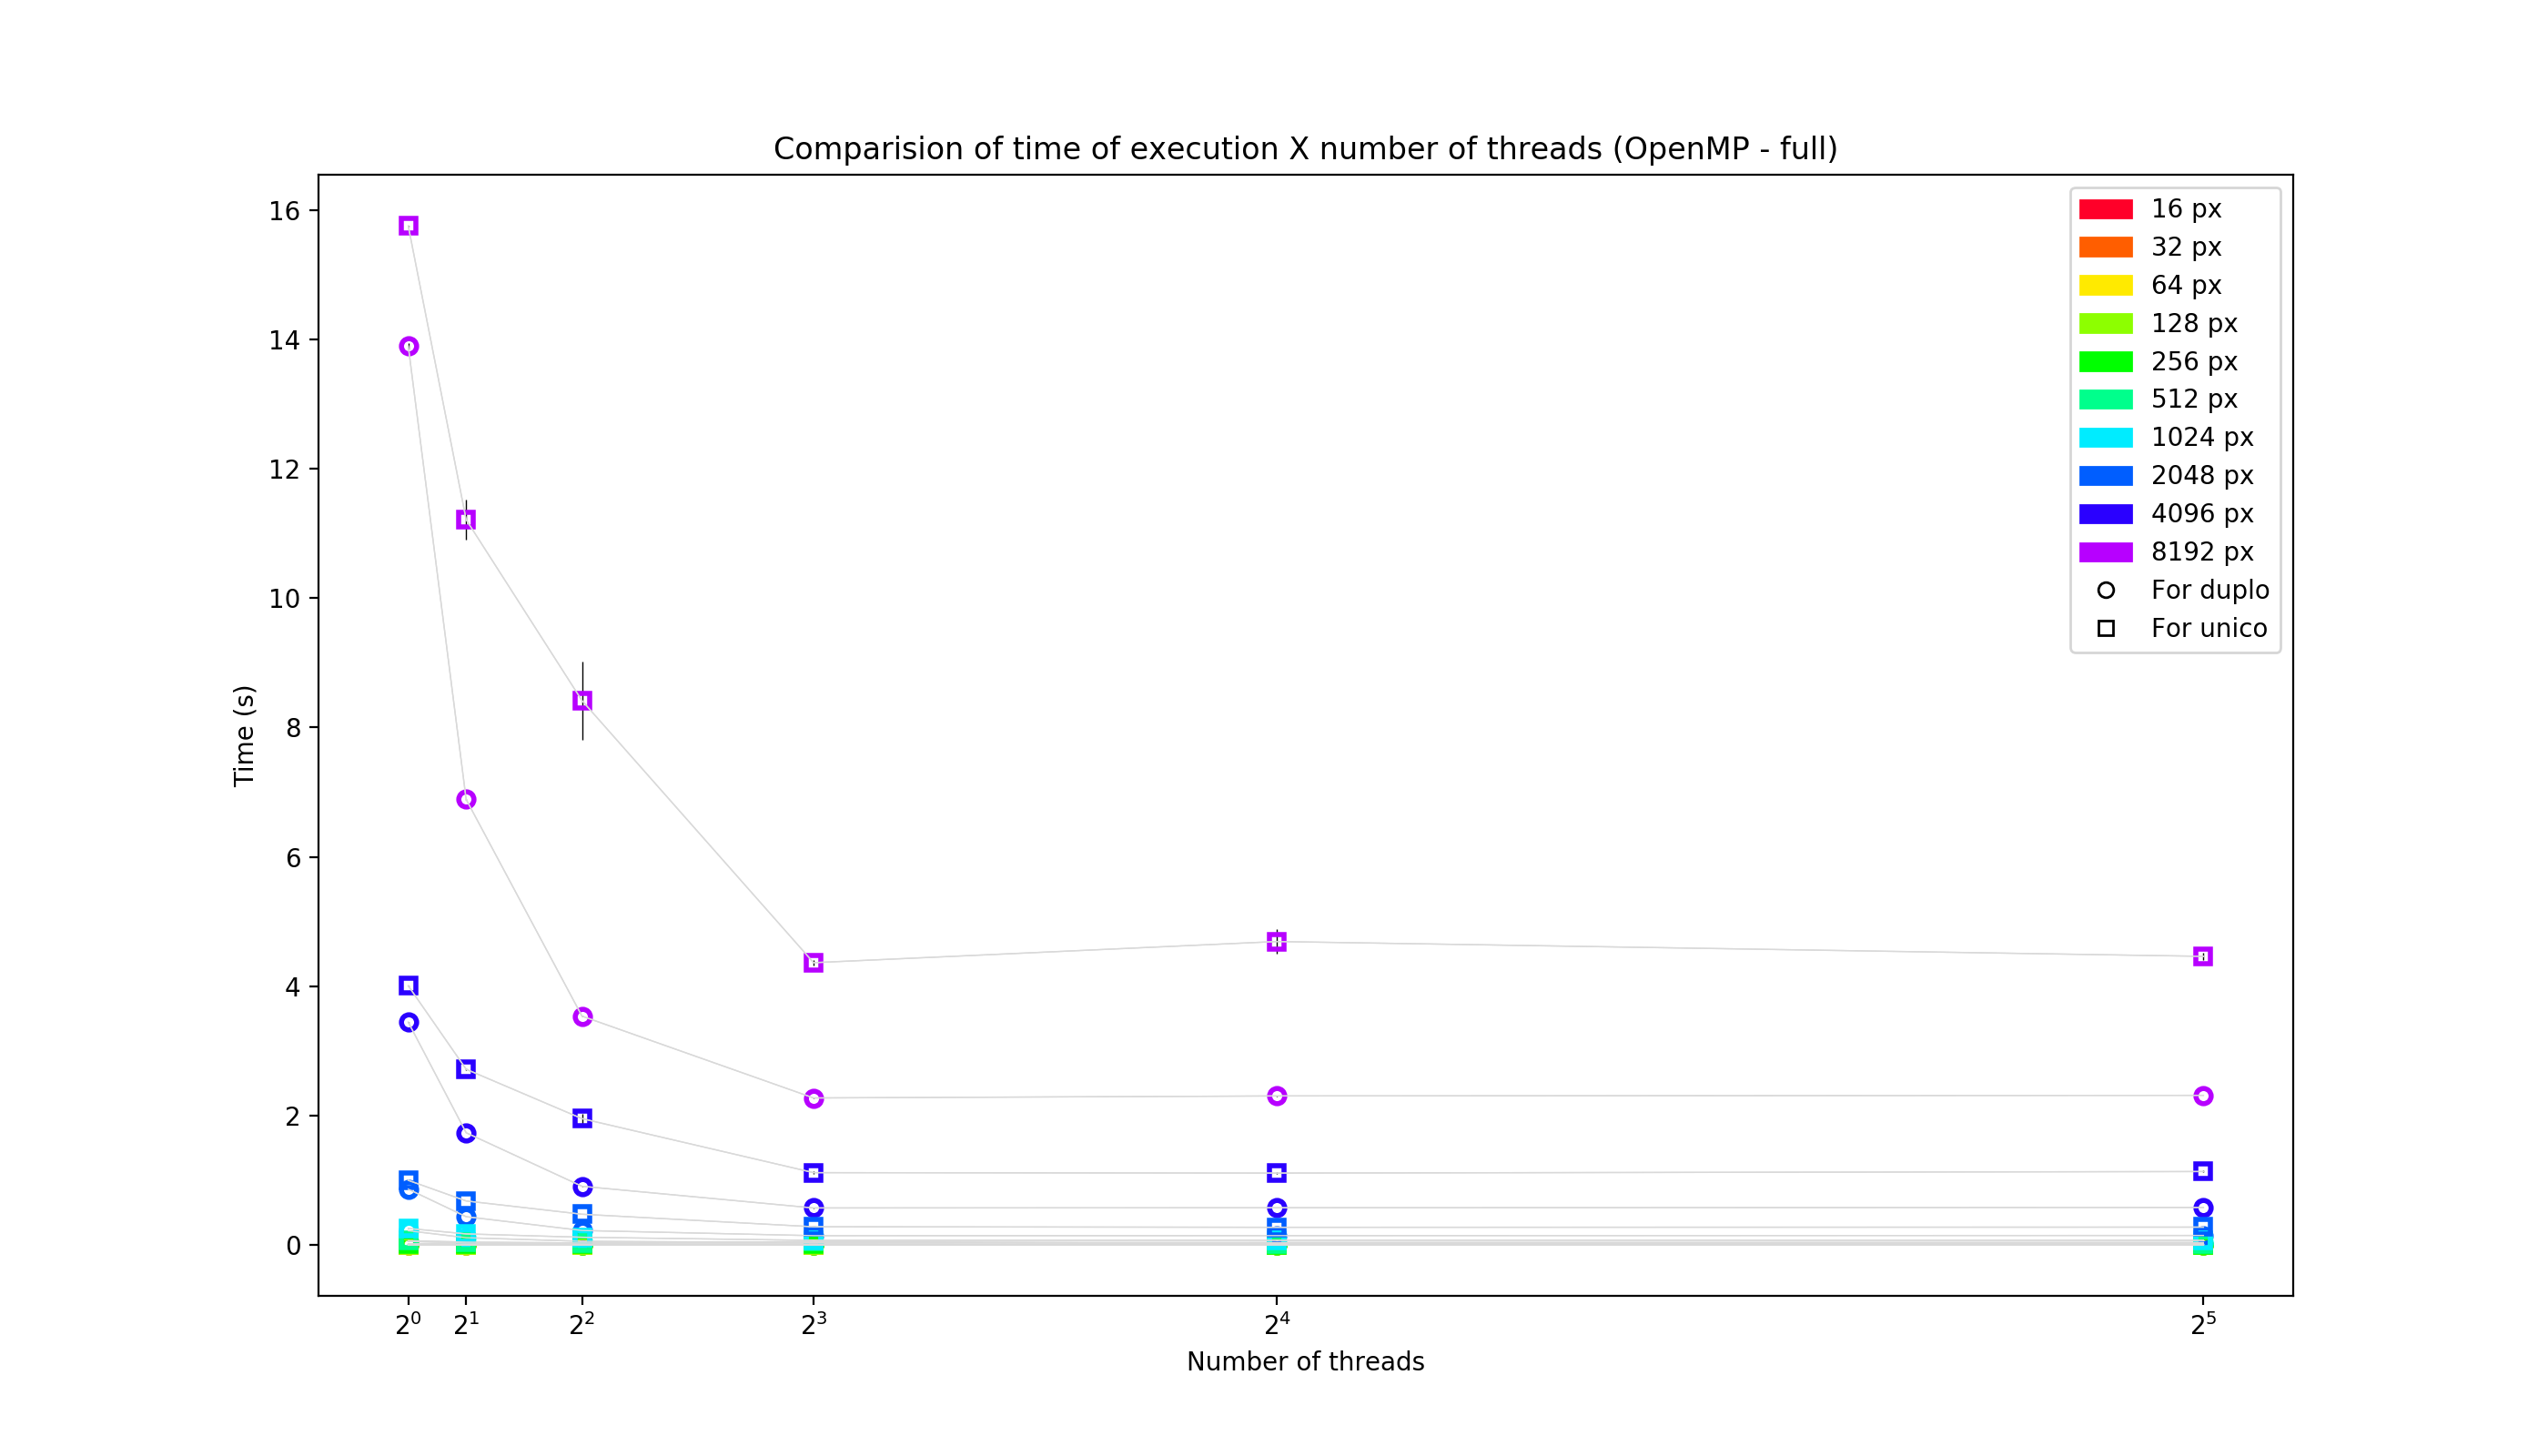
\includegraphics[scale=.55]{for_duploXunico/compare_timeXthread_full_OpenMPpng.png}}
\end{figure}

\begin{figure}[H]
    \makebox[\textwidth][c]{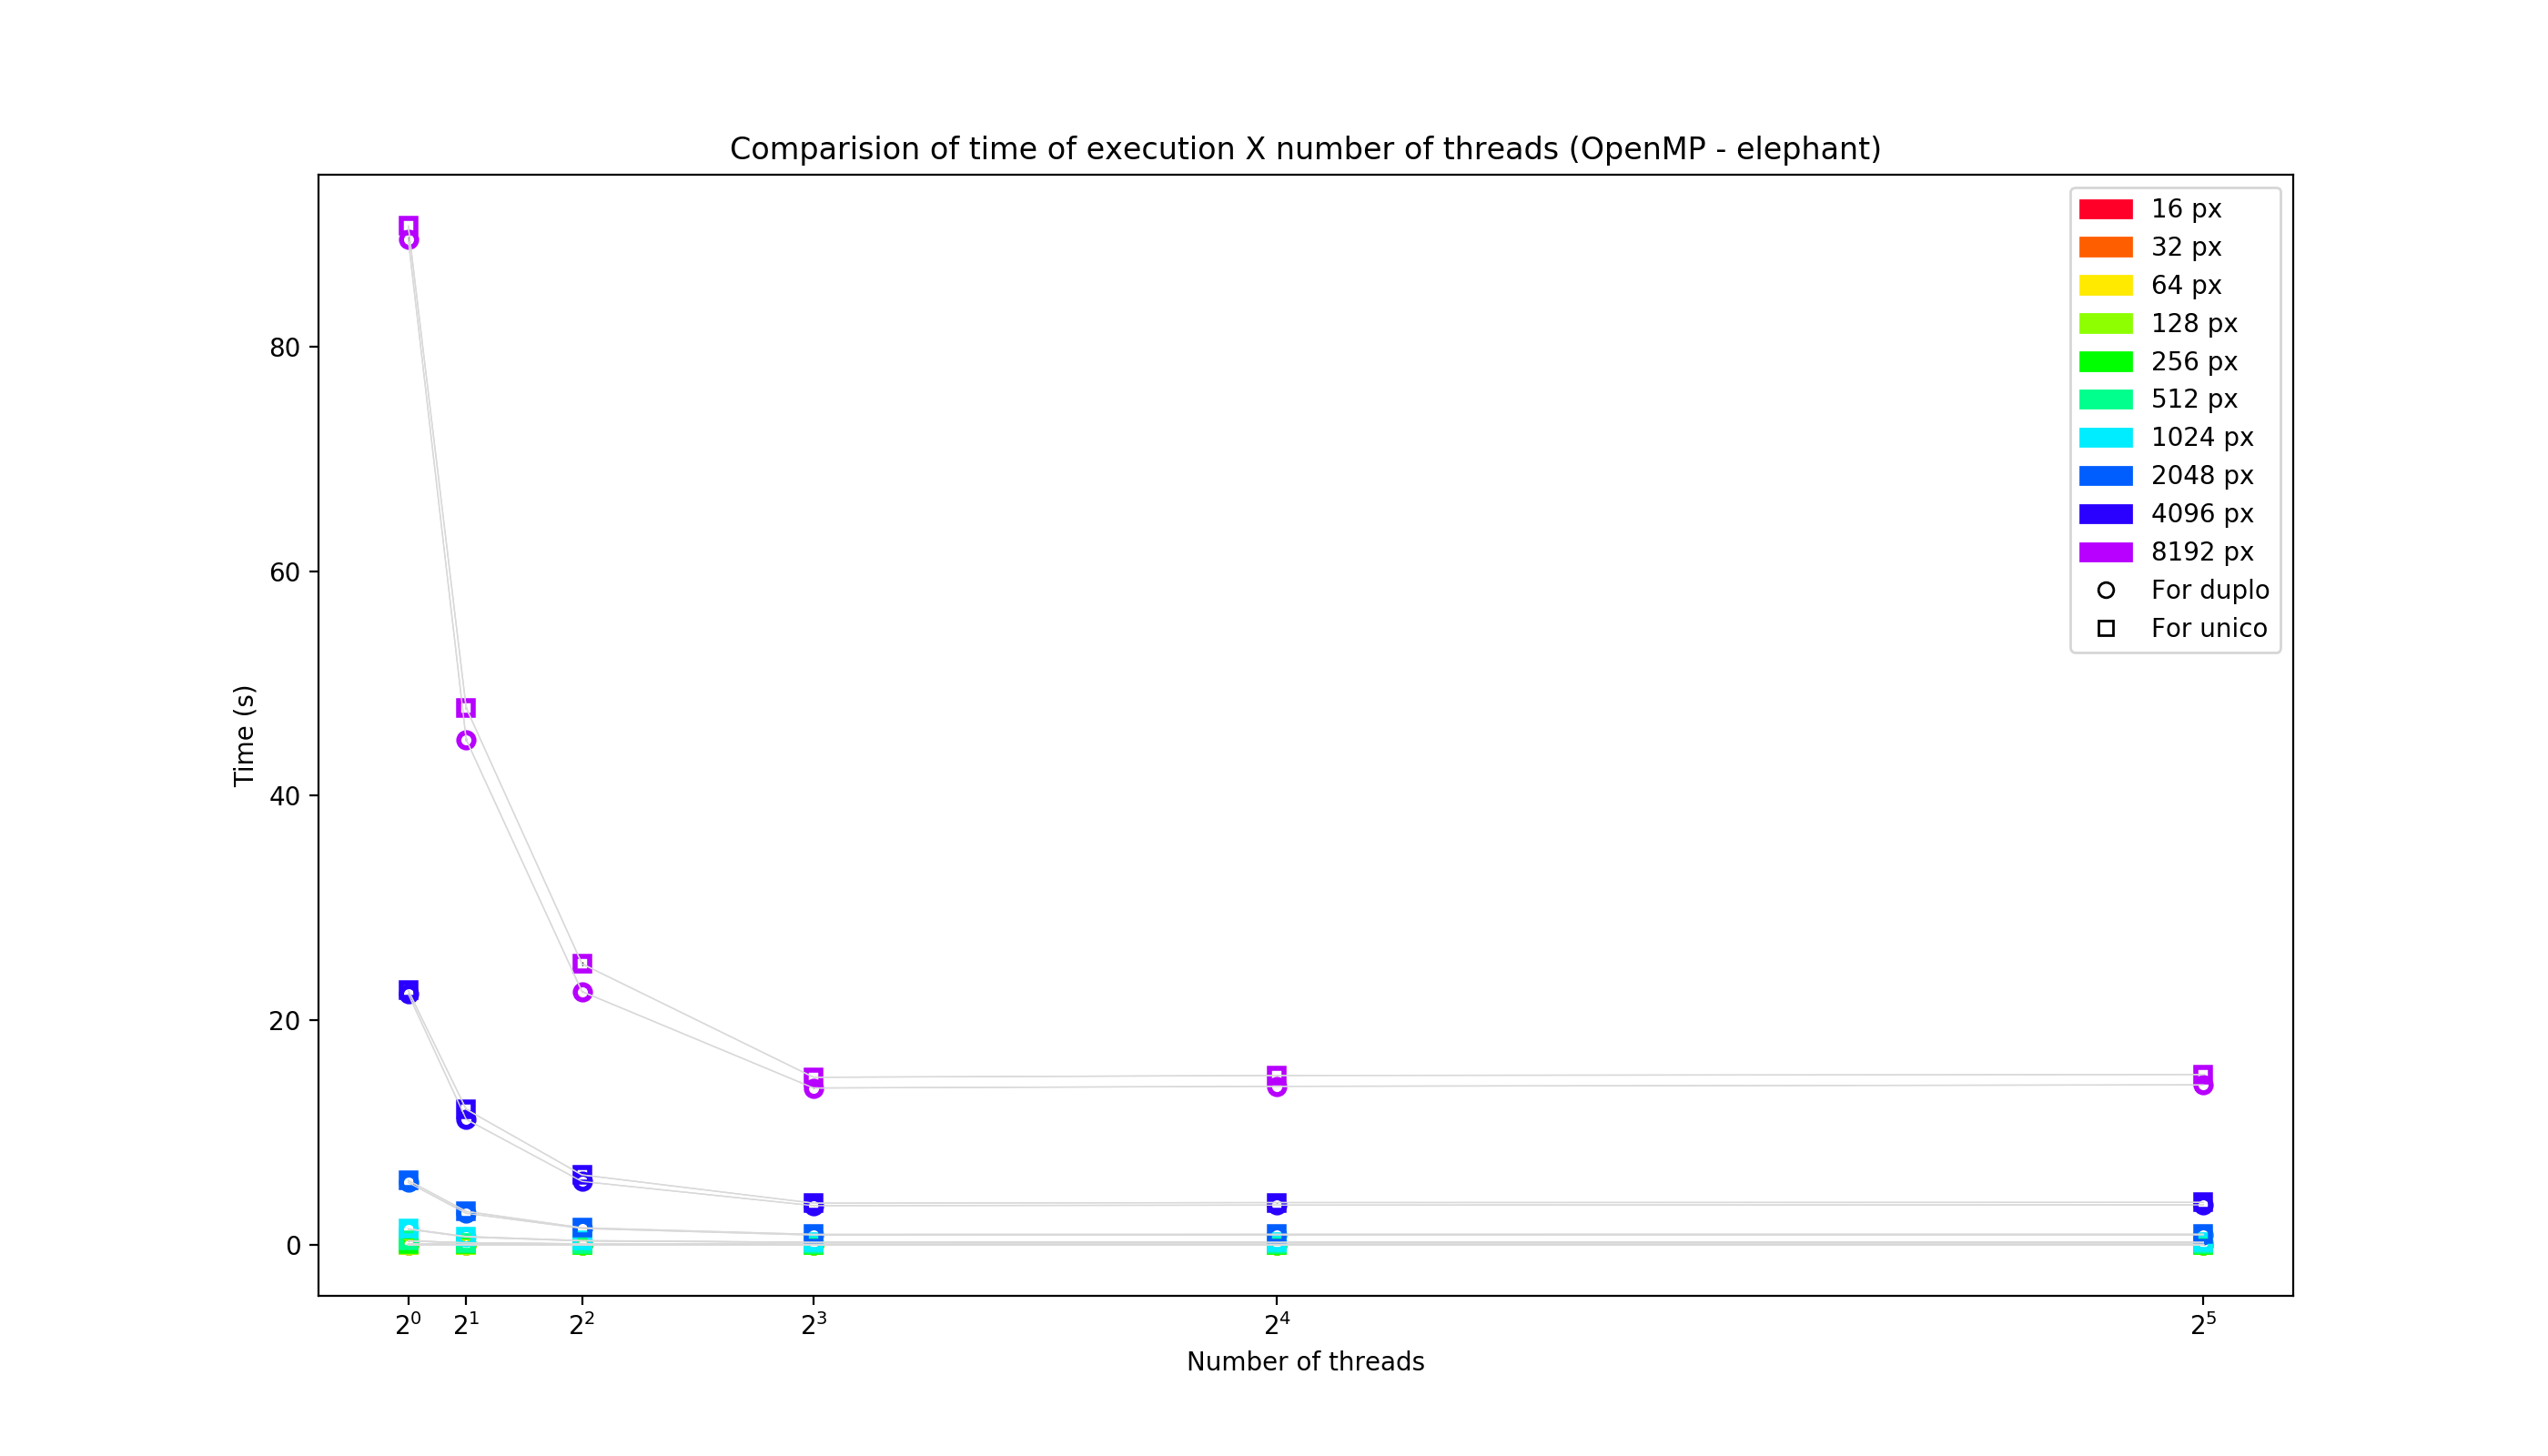
\includegraphics[scale=.55]{for_duploXunico/compare_timeXthread_elephant_OpenMPpng.png}}
\end{figure}

\begin{figure}[H]
    \makebox[\textwidth][c]{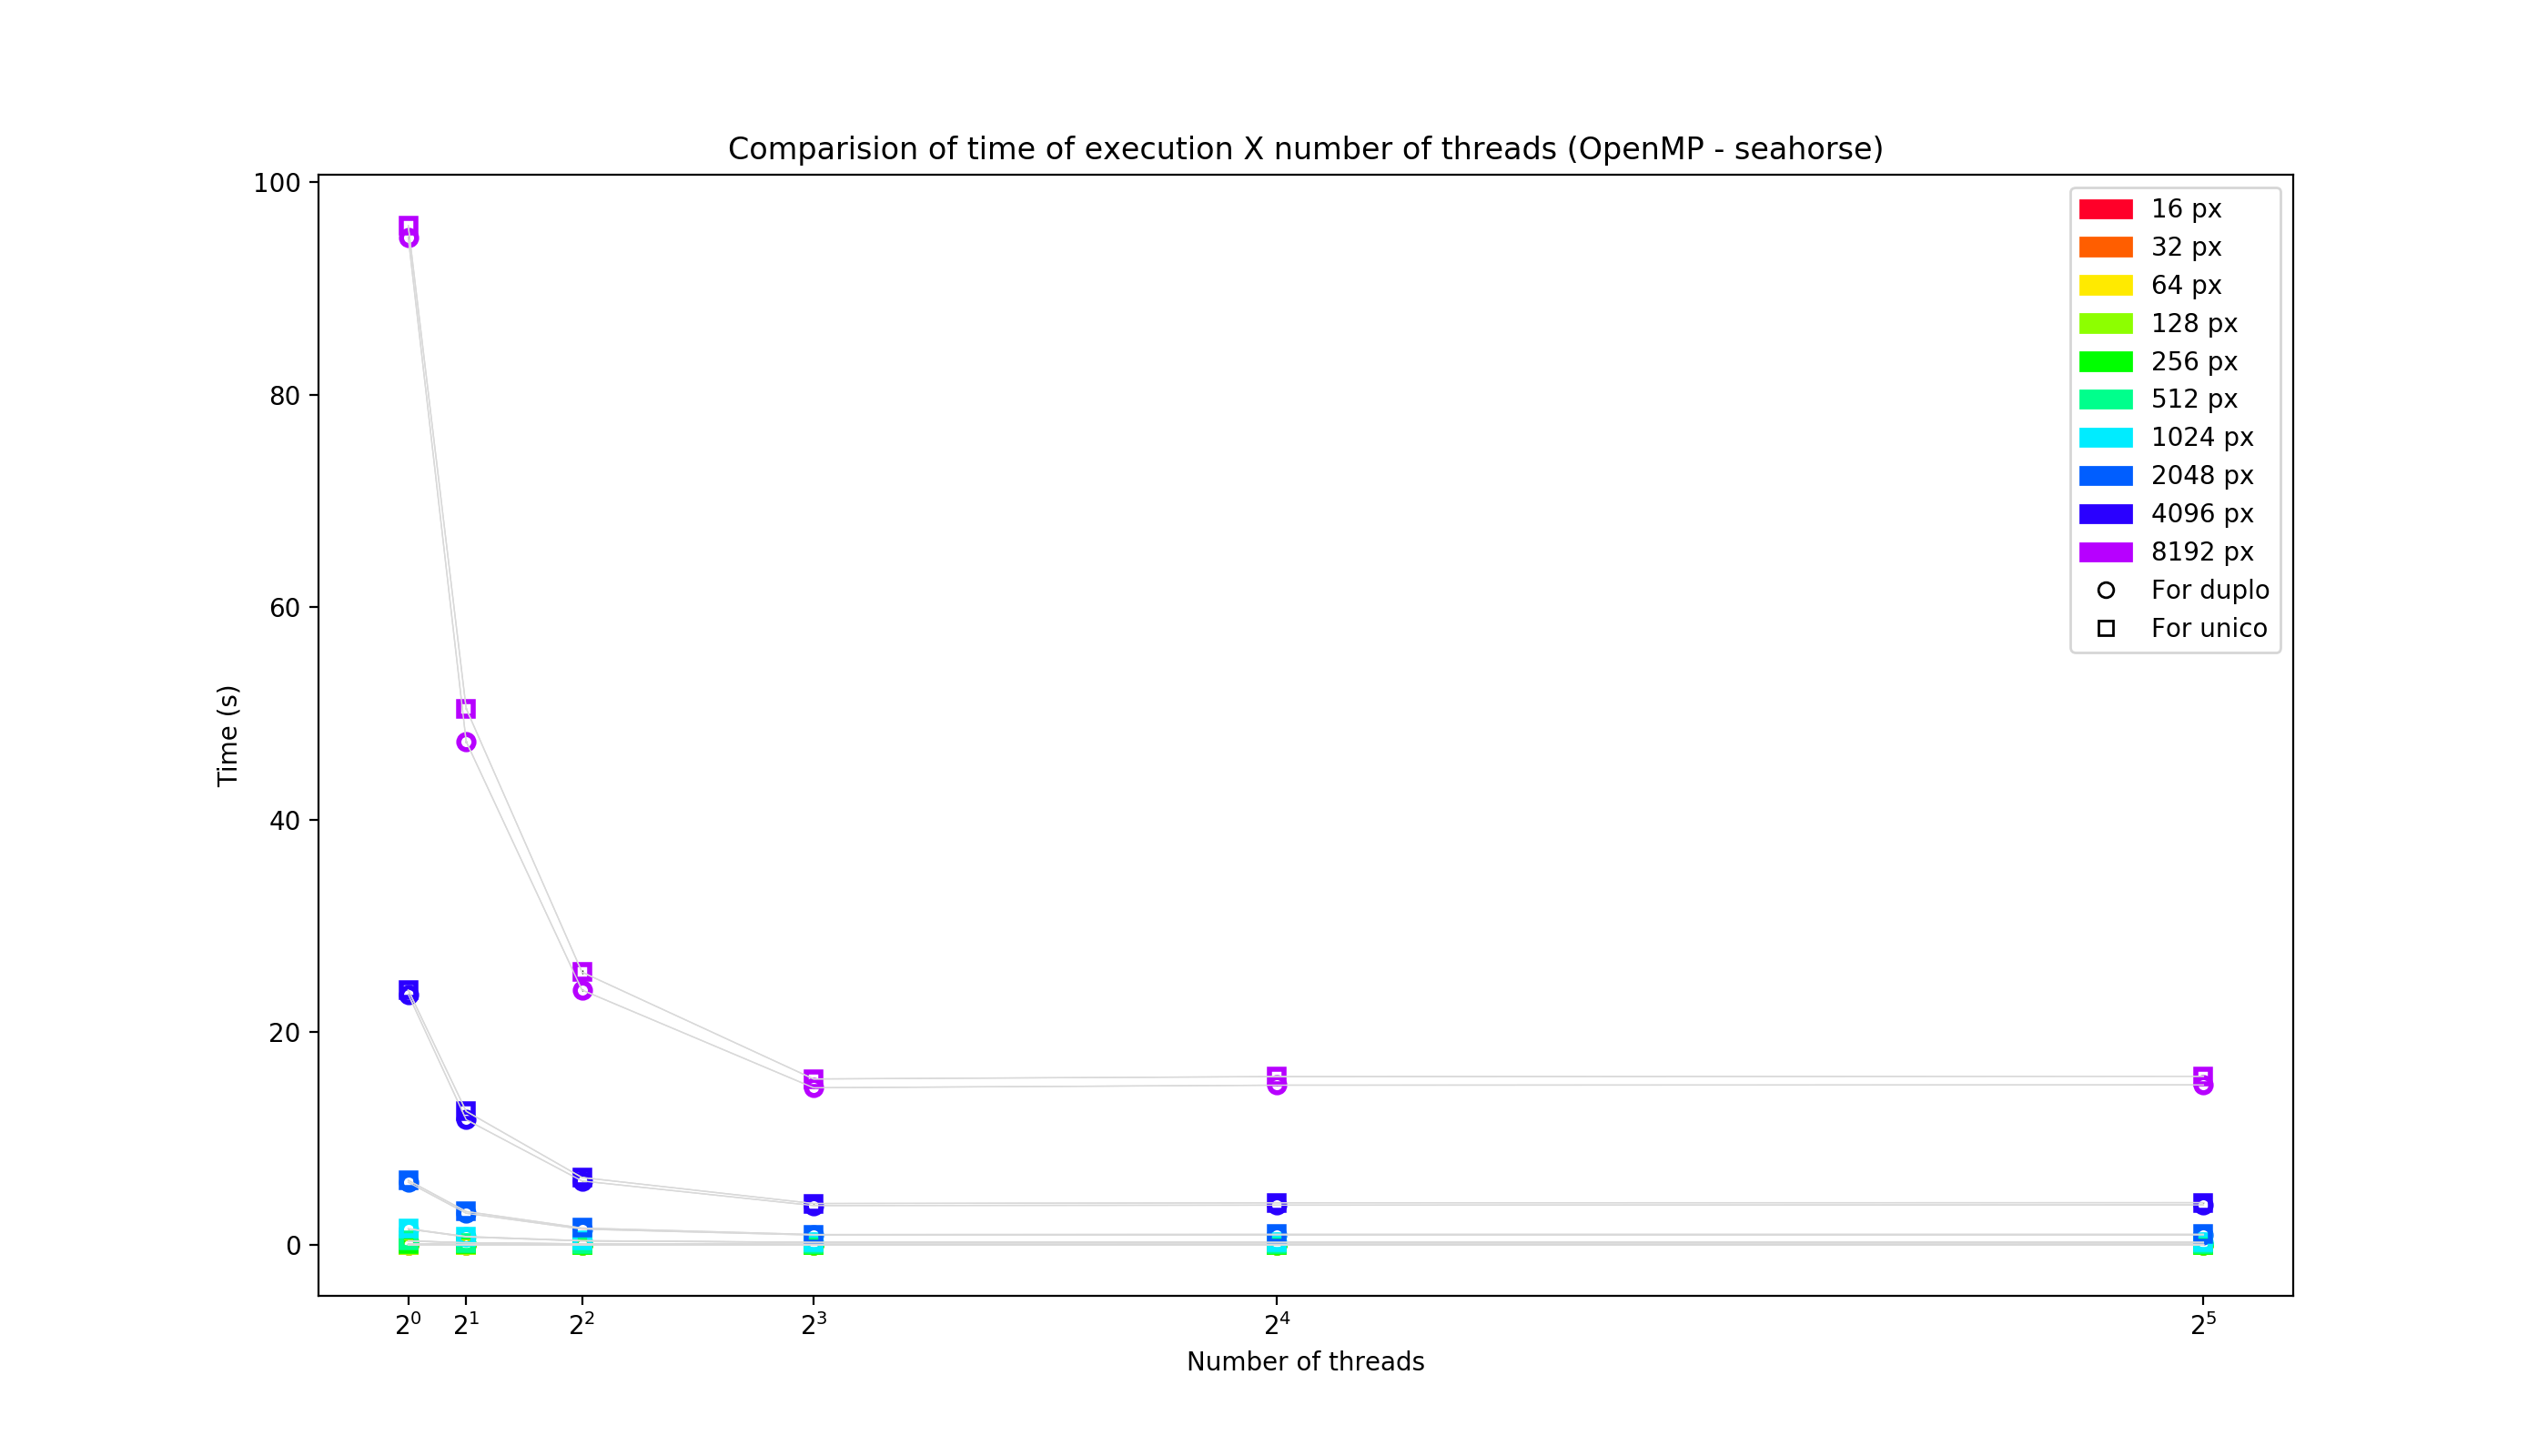
\includegraphics[scale=.55]{for_duploXunico/compare_timeXthread_seahorse_OpenMPpng.png}}
\end{figure}

\begin{figure}[H]
    \makebox[\textwidth][c]{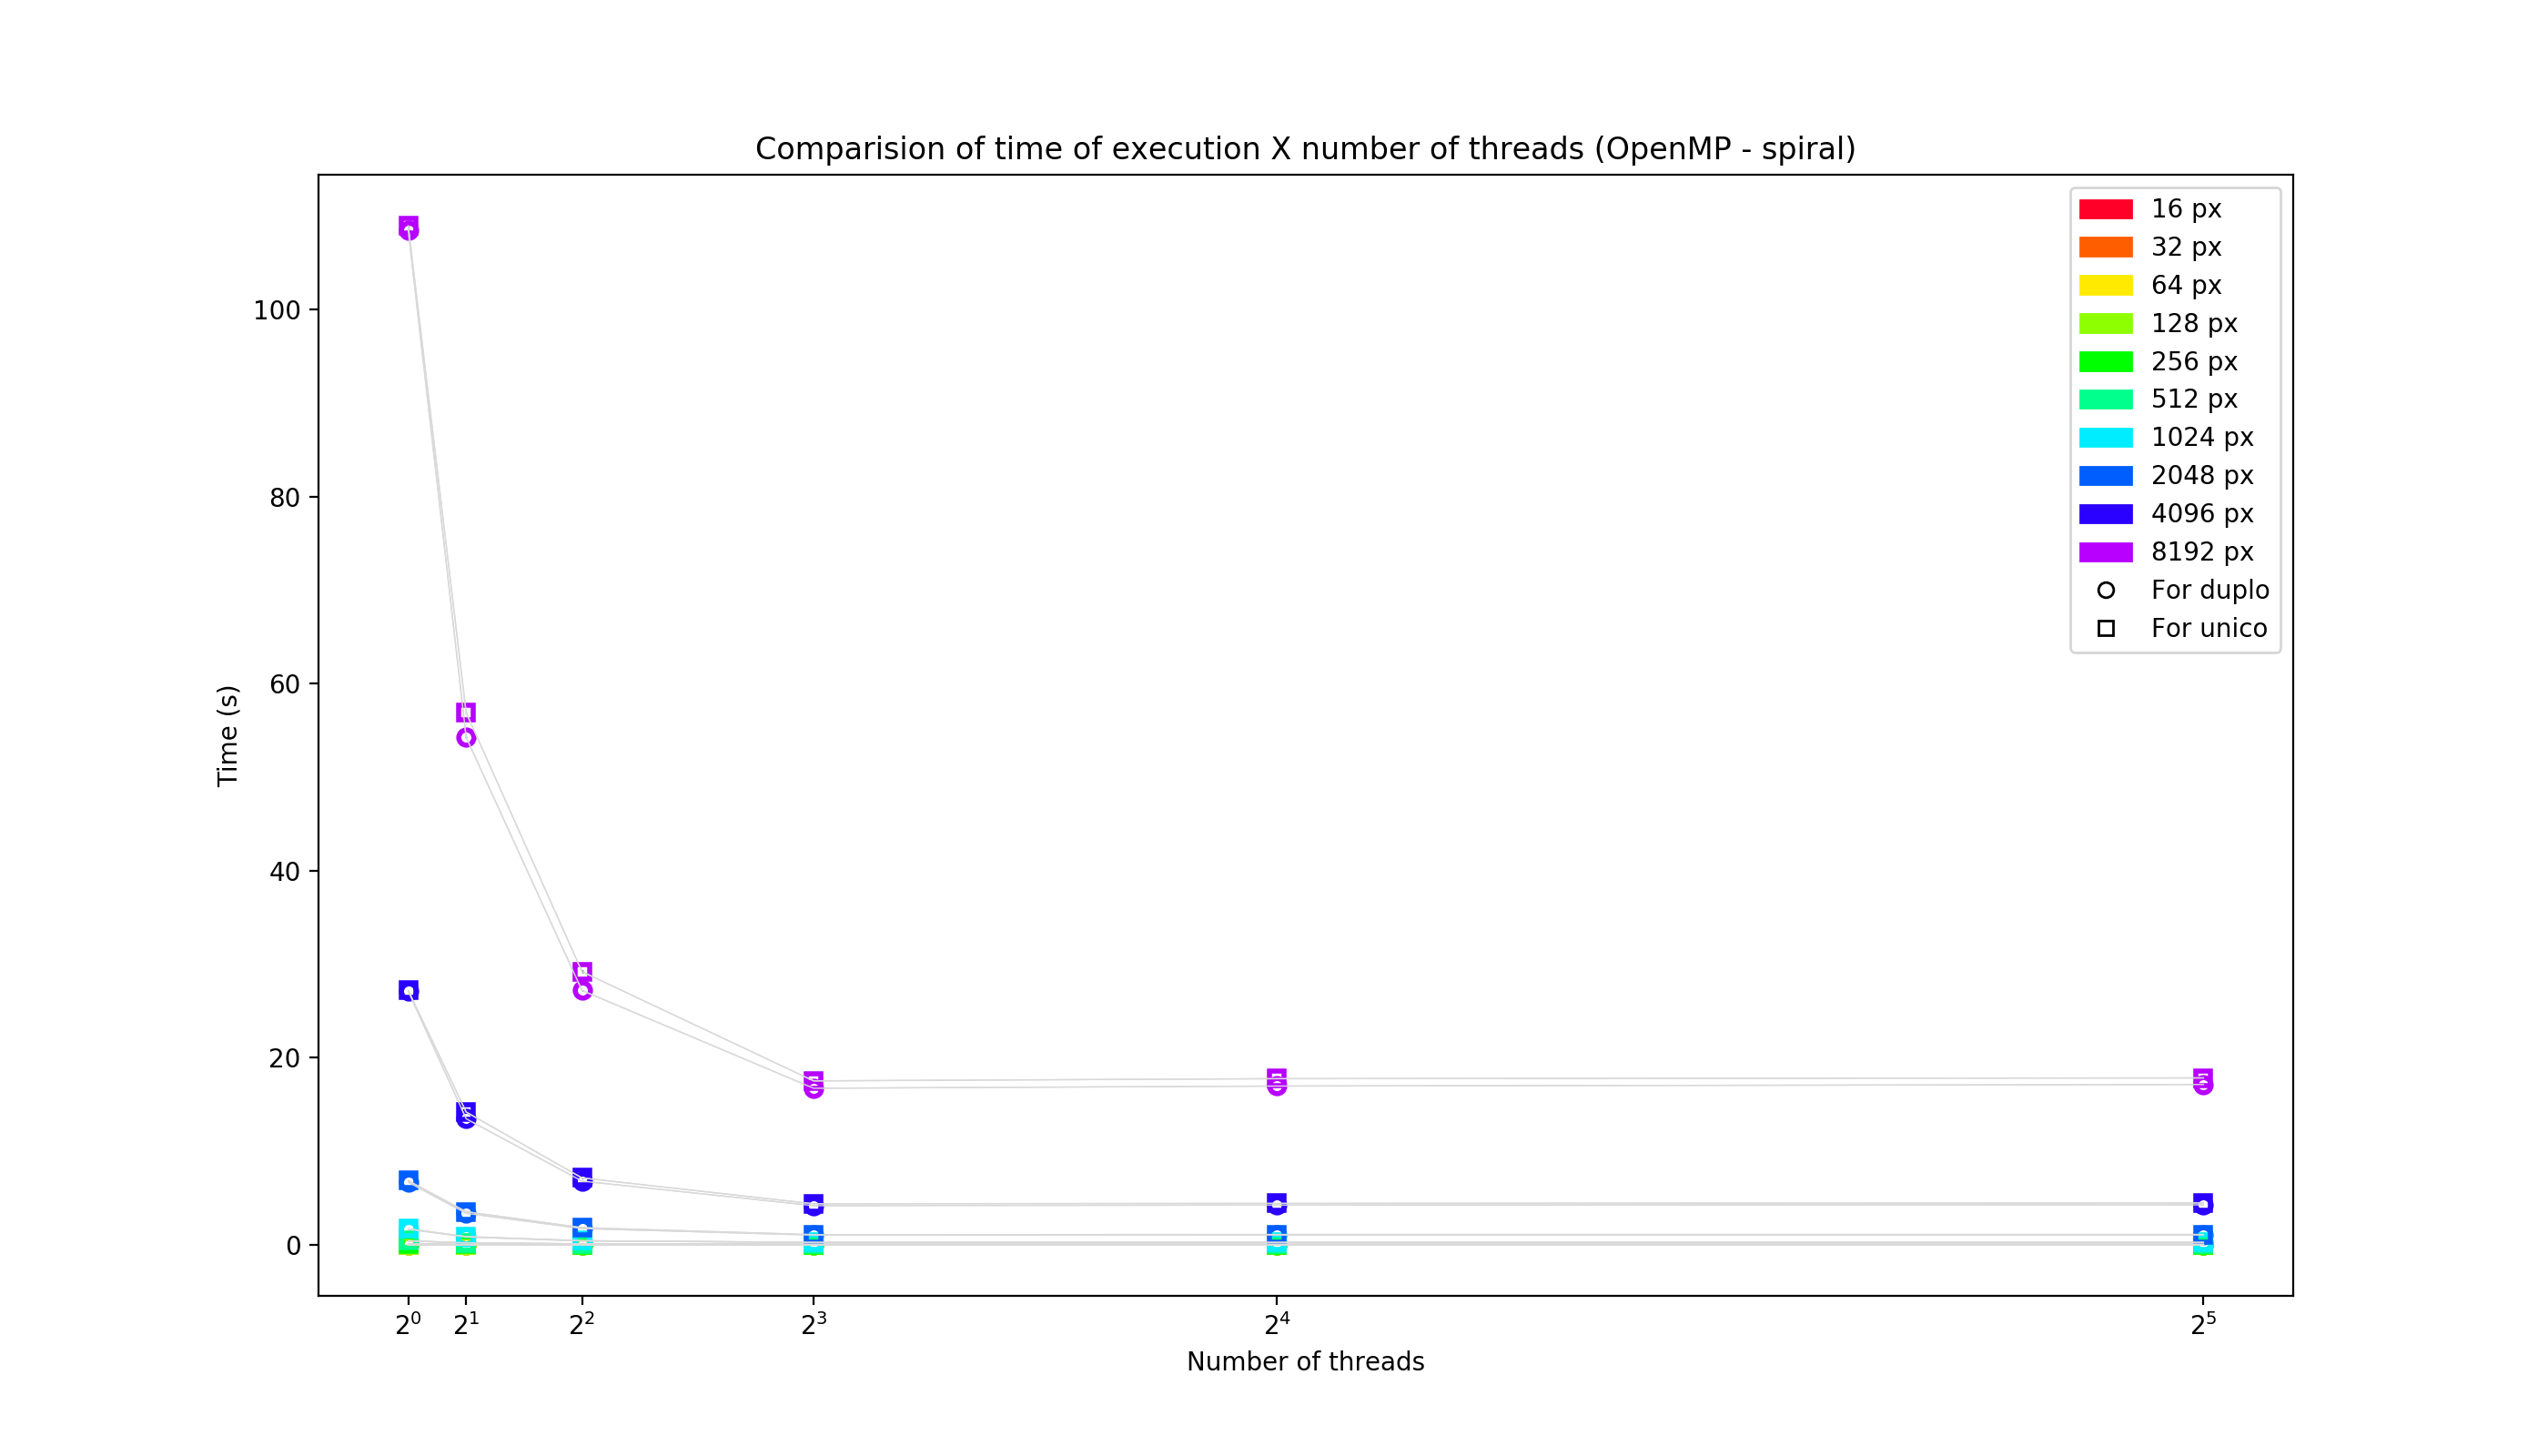
\includegraphics[scale=.55]{for_duploXunico/compare_timeXthread_spiral_OpenMPpng.png}}
\end{figure}

Para o caso da região full nota-se que em todos os casos a versão com dois fors foi mais rápida que a versão com somente um. Apesar do gráfico da região Full parecer que há mais variação também devemos lembrar que o eixo Y dela vai de 0 a 16, enquanto os demais ultrapassam 80. Se verificarmos as diferenças entre tempos com o mesmo número de threads, haverá sempre uma diferença semelhante em todas as regiões.
Como talvez o problema sejam os chunks sejam muito pequenos e por conta disso o programa gaste muito tempo fazendo troca de contexto, o próximo experimento foi feito com chunks maiores. Dividimos o número de interações do for pelo número de threads, isto é, cada thread terá um chunk para sí:
\begin{lstlisting}[style=CStyle]
    #pragma omp parallel for private(...) num_threads(nThreads) schedule(dynamic, i_y_max * i_x_max / nThreads)
    for (i = 0; i < i_y_max * i_x_max; i++) {
        i_y = i / i_y_max;
        i_x = i % i_y_max;
        ...
\end{lstlisting}

No entanto os resultados ainda foram piores do que o for duplo com \code{schedule(dynamic)}:

\begin{figure}[H]
    \makebox[\textwidth][c]{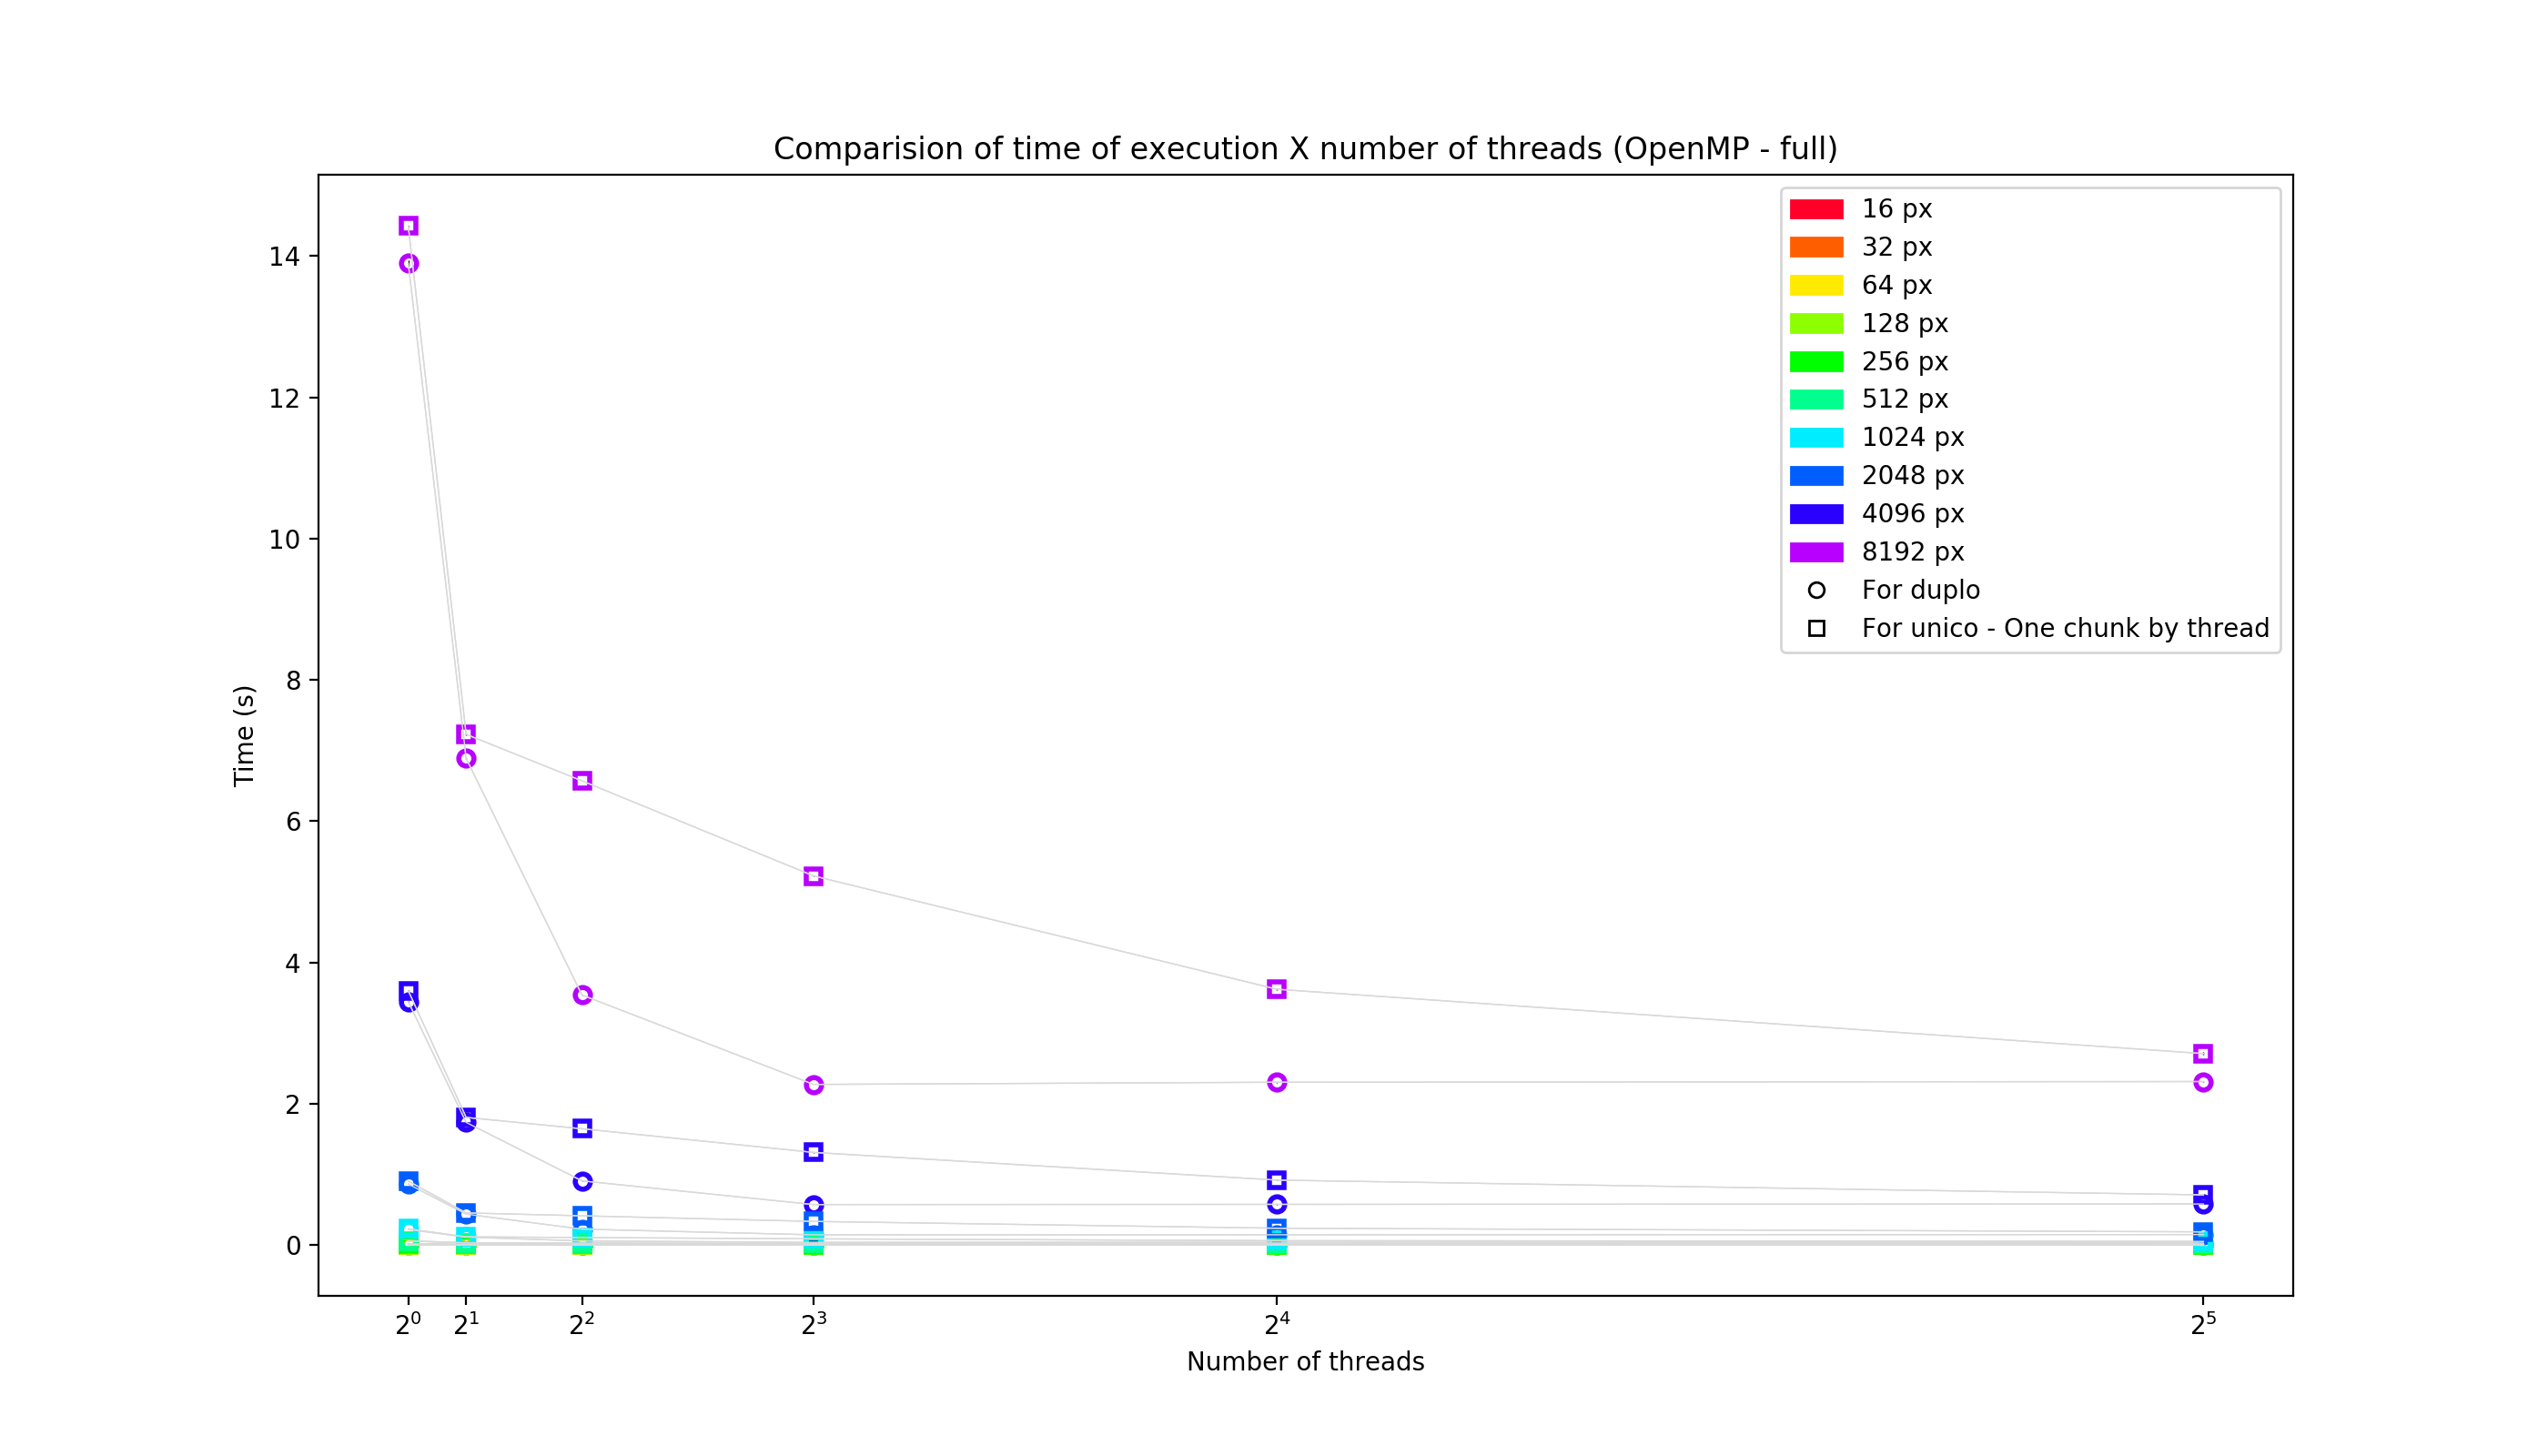
\includegraphics[scale=.55]{for_duploXunico_bigbig/compare_timeXthread_full_OpenMPpng.png}}
\end{figure}

\begin{figure}[H]
    \makebox[\textwidth][c]{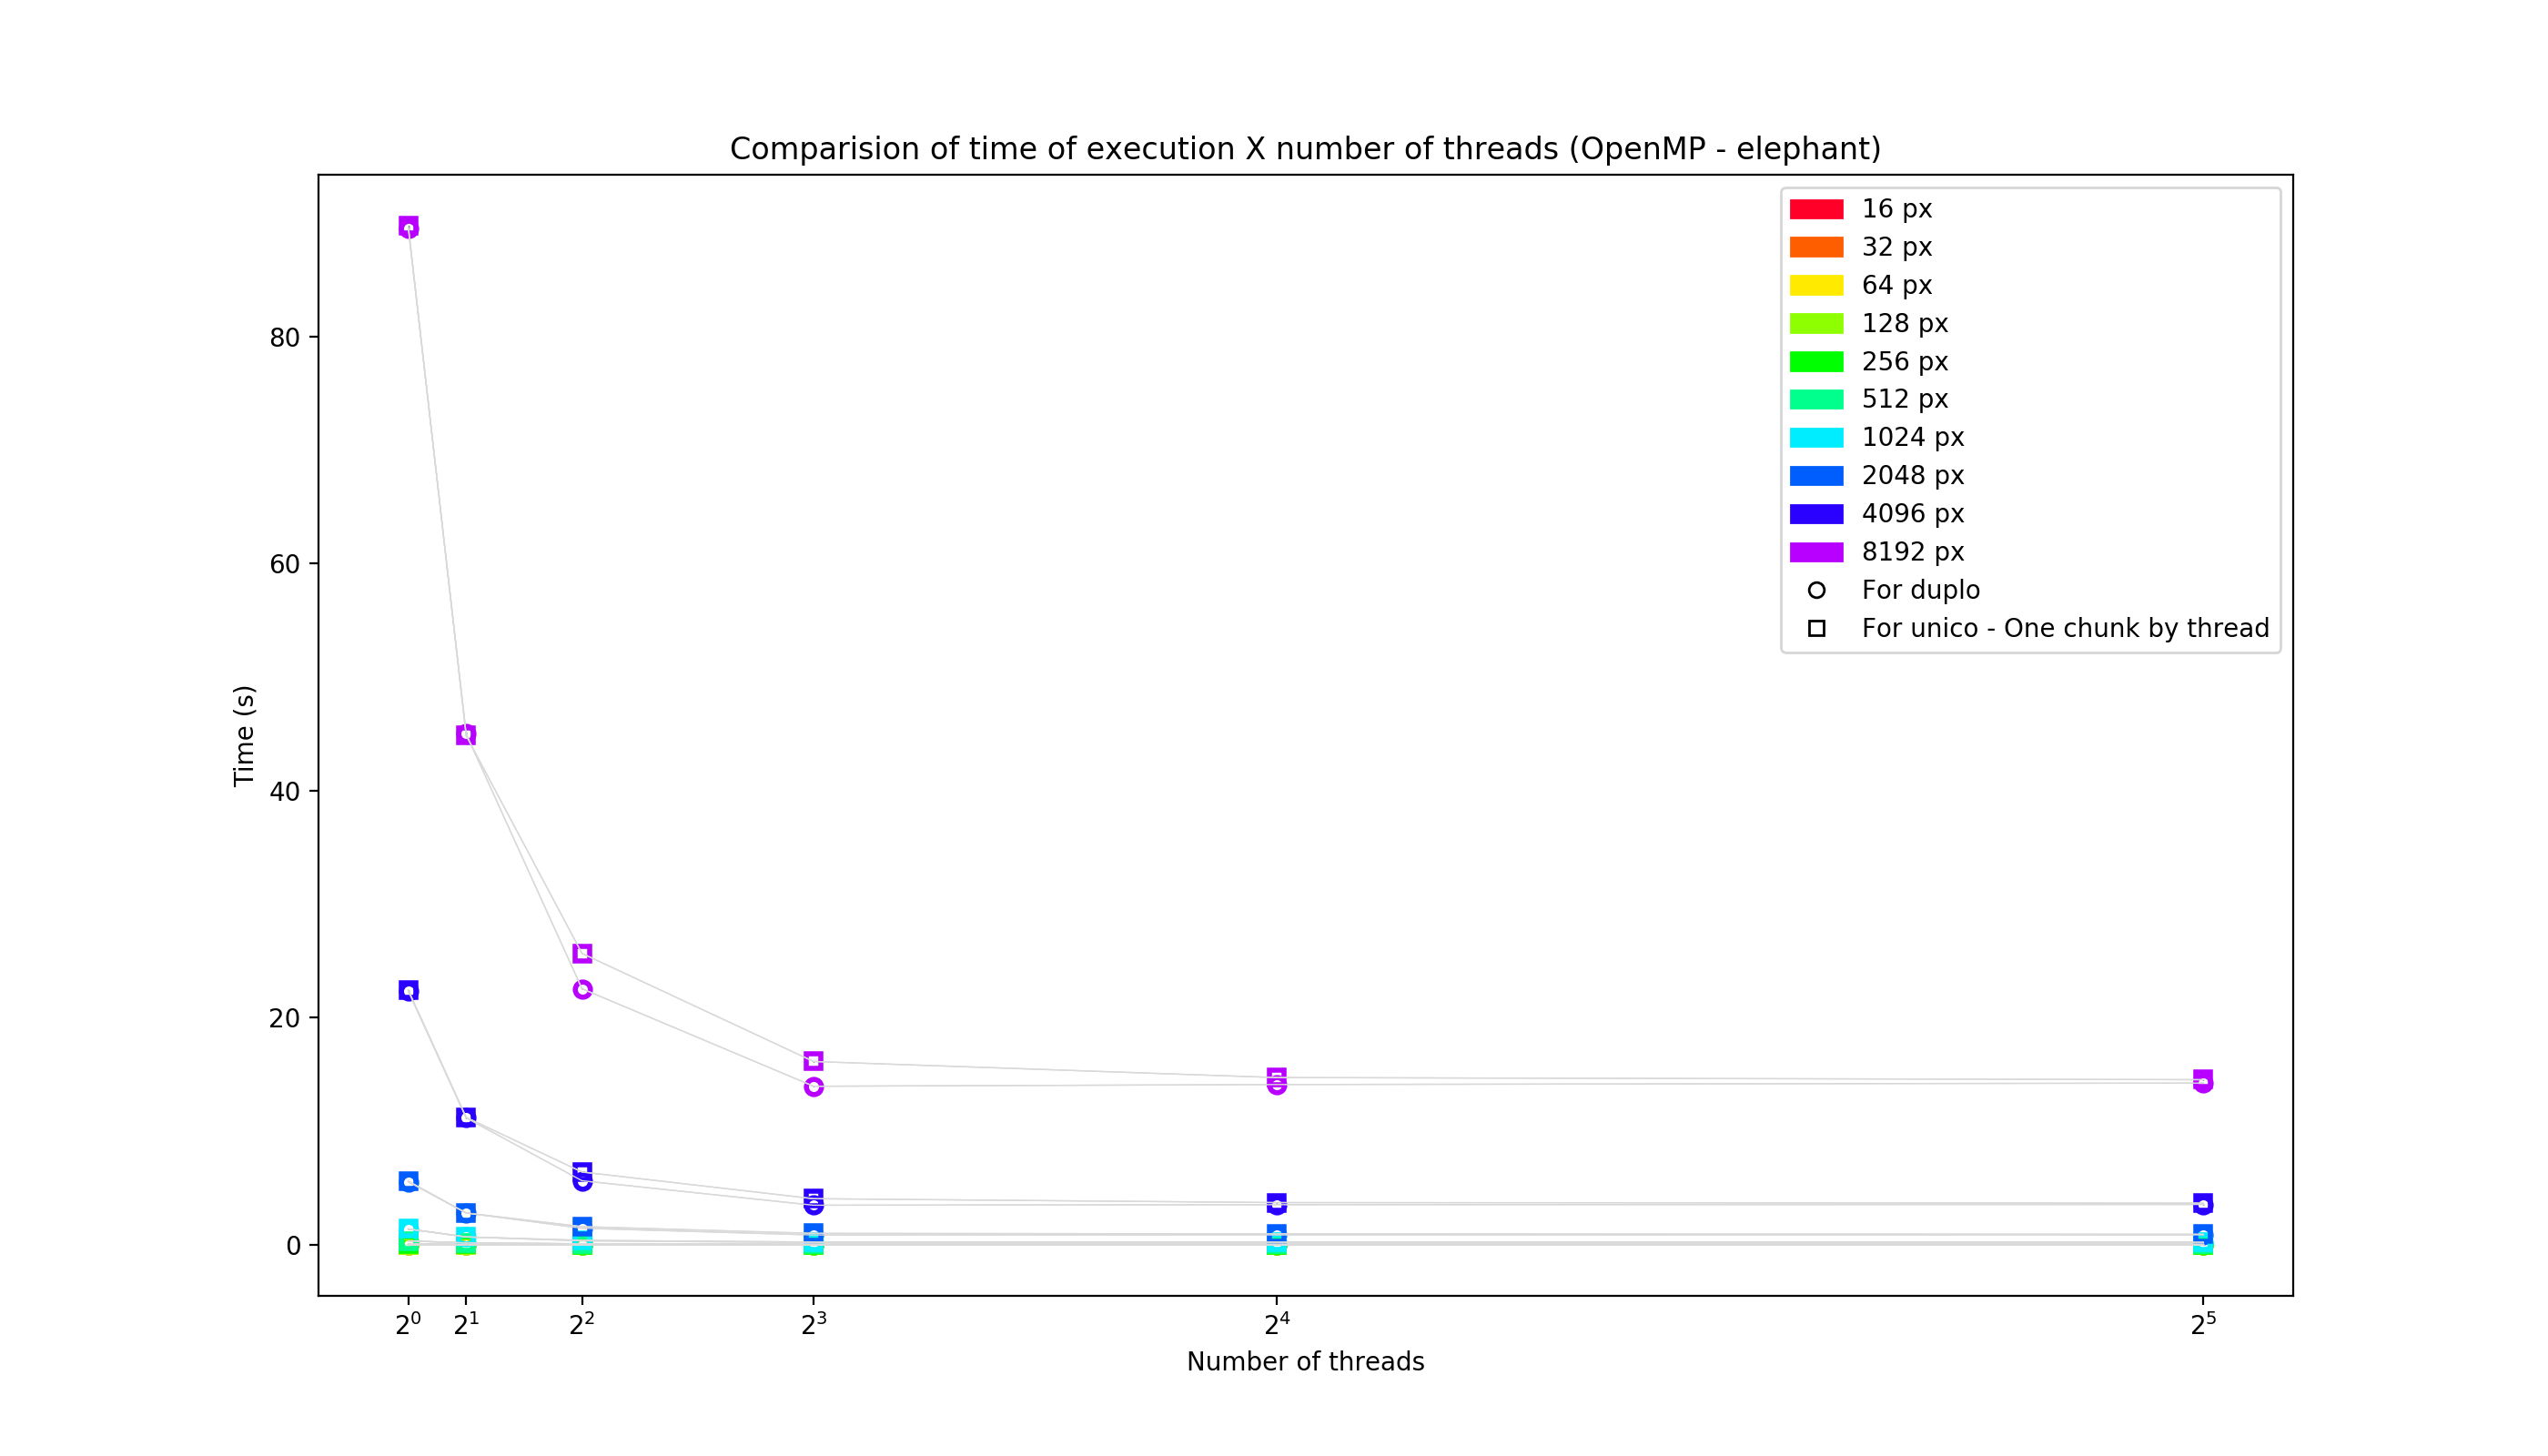
\includegraphics[scale=.55]{for_duploXunico_bigbig/compare_timeXthread_elephant_OpenMPpng.png}}
\end{figure}

\begin{figure}[H]
    \makebox[\textwidth][c]{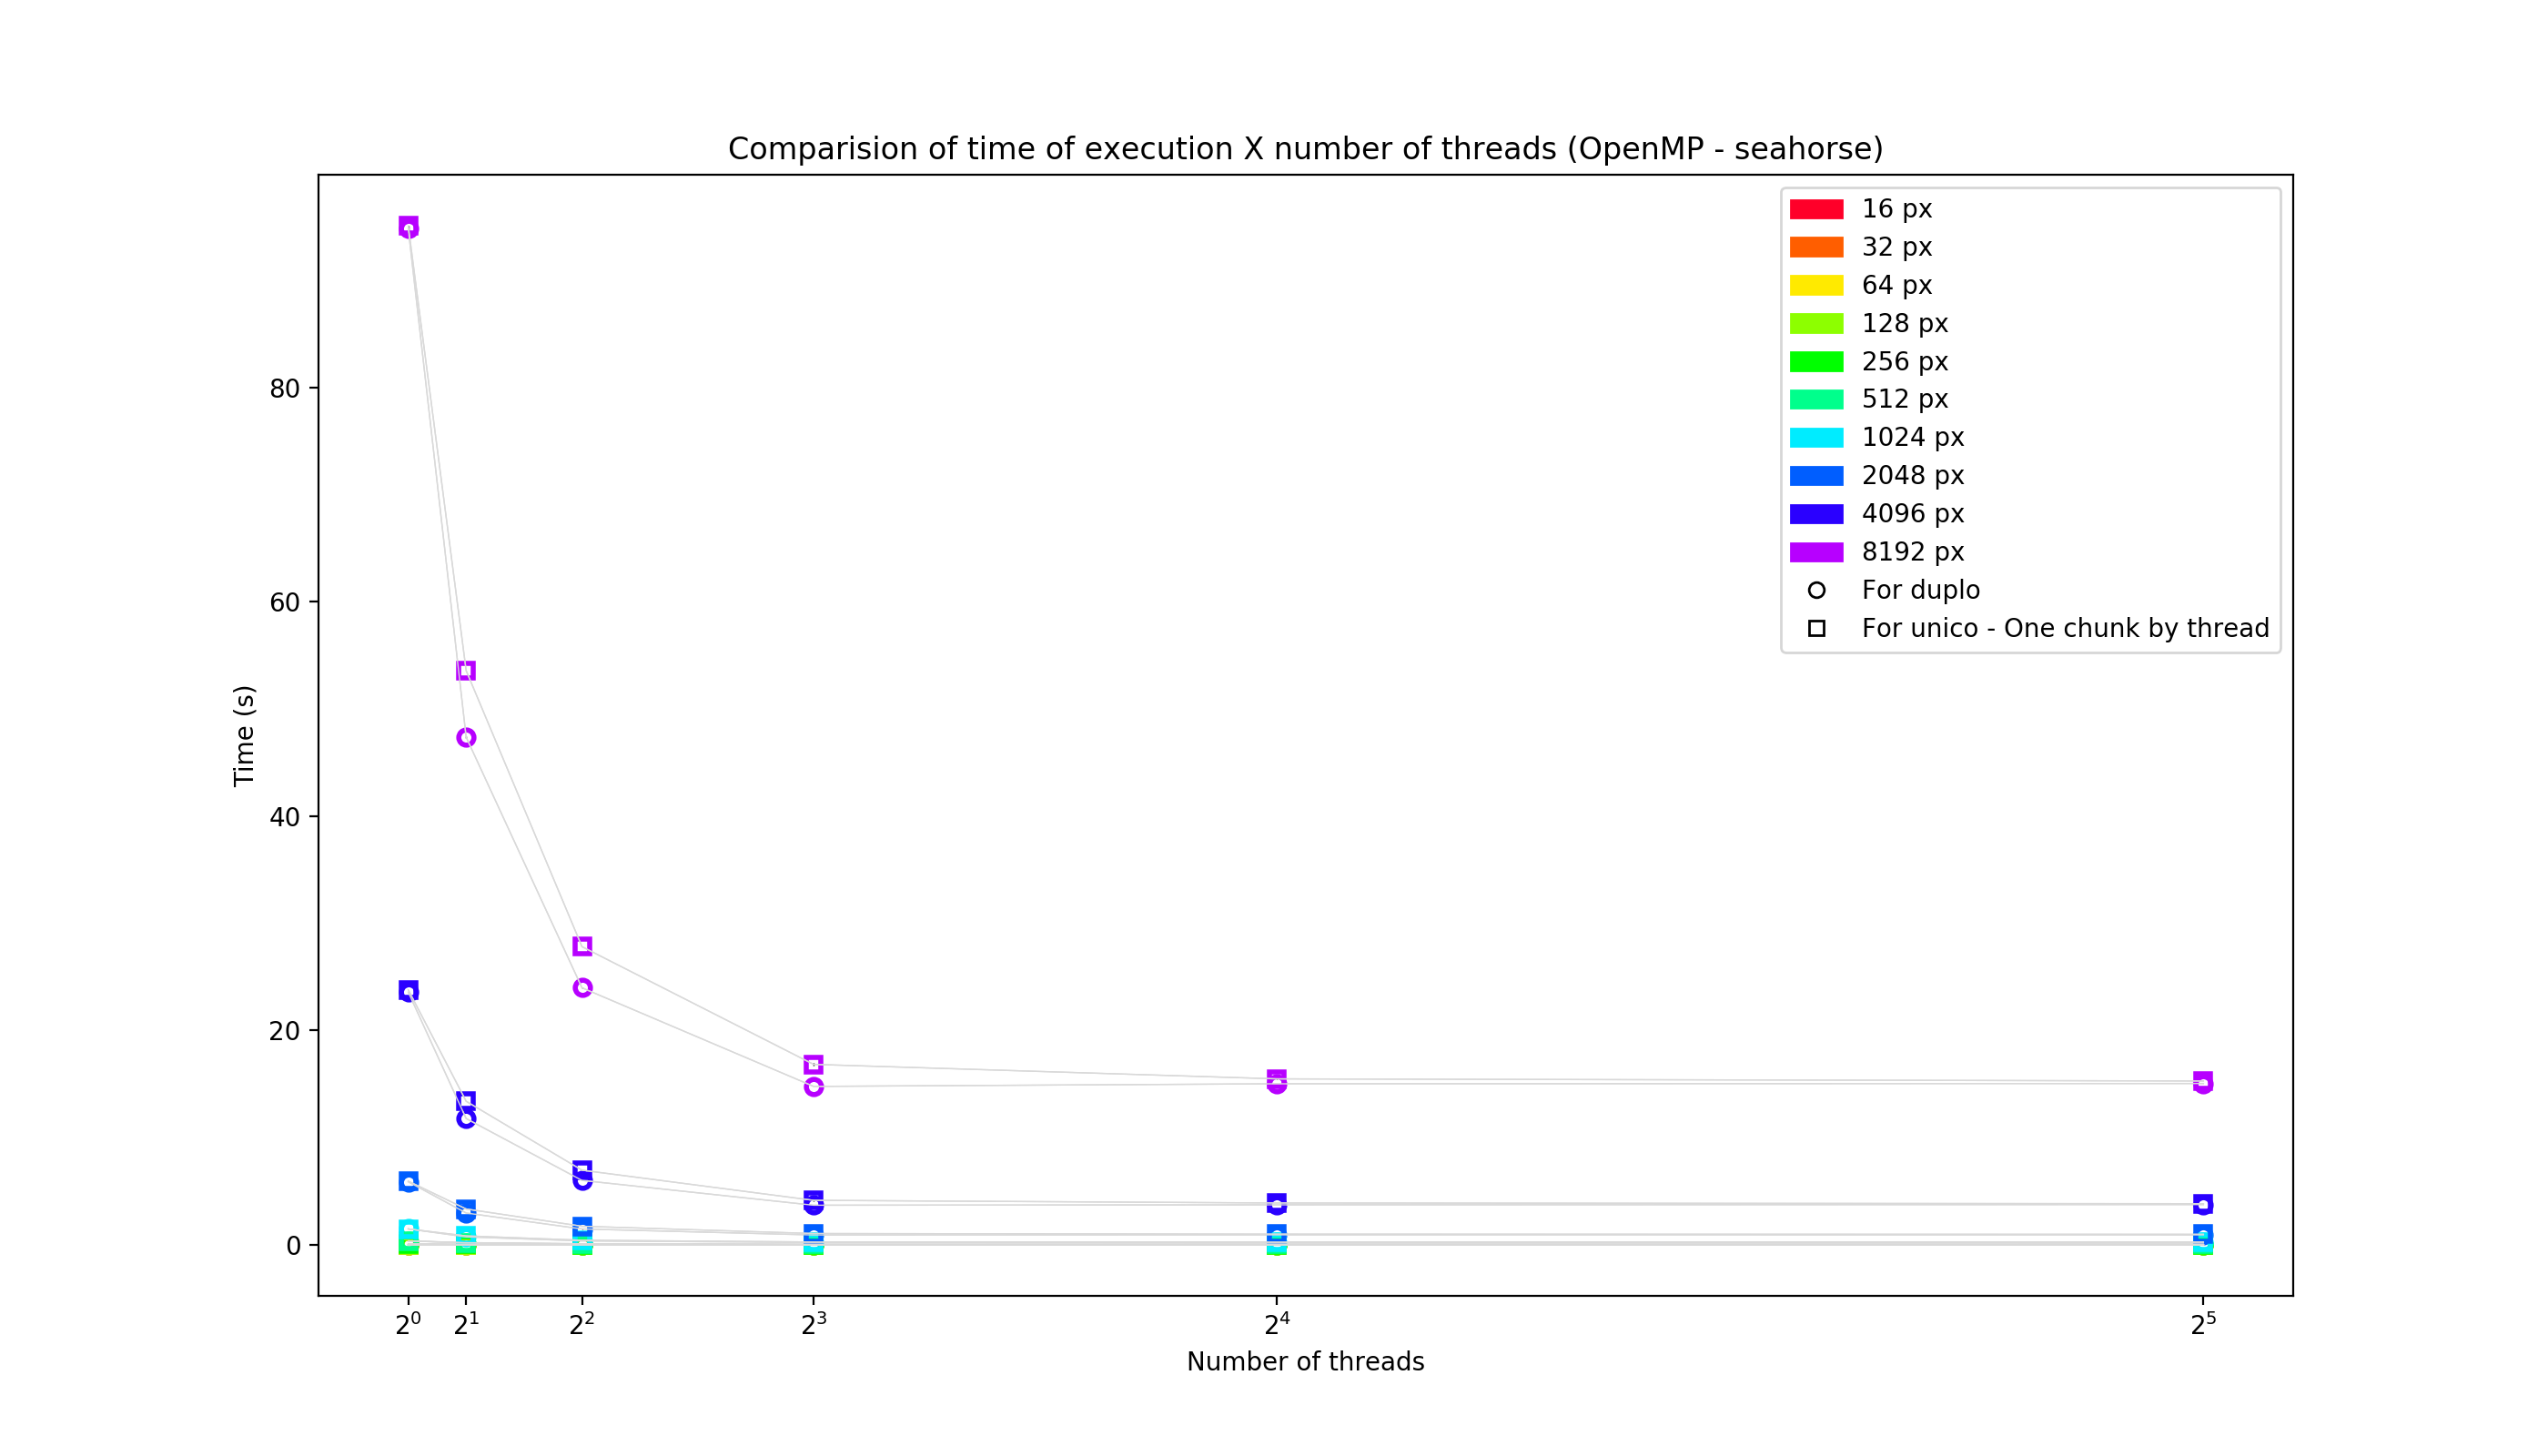
\includegraphics[scale=.55]{for_duploXunico_bigbig/compare_timeXthread_seahorse_OpenMPpng.png}}
\end{figure}

\begin{figure}[H]
    \makebox[\textwidth][c]{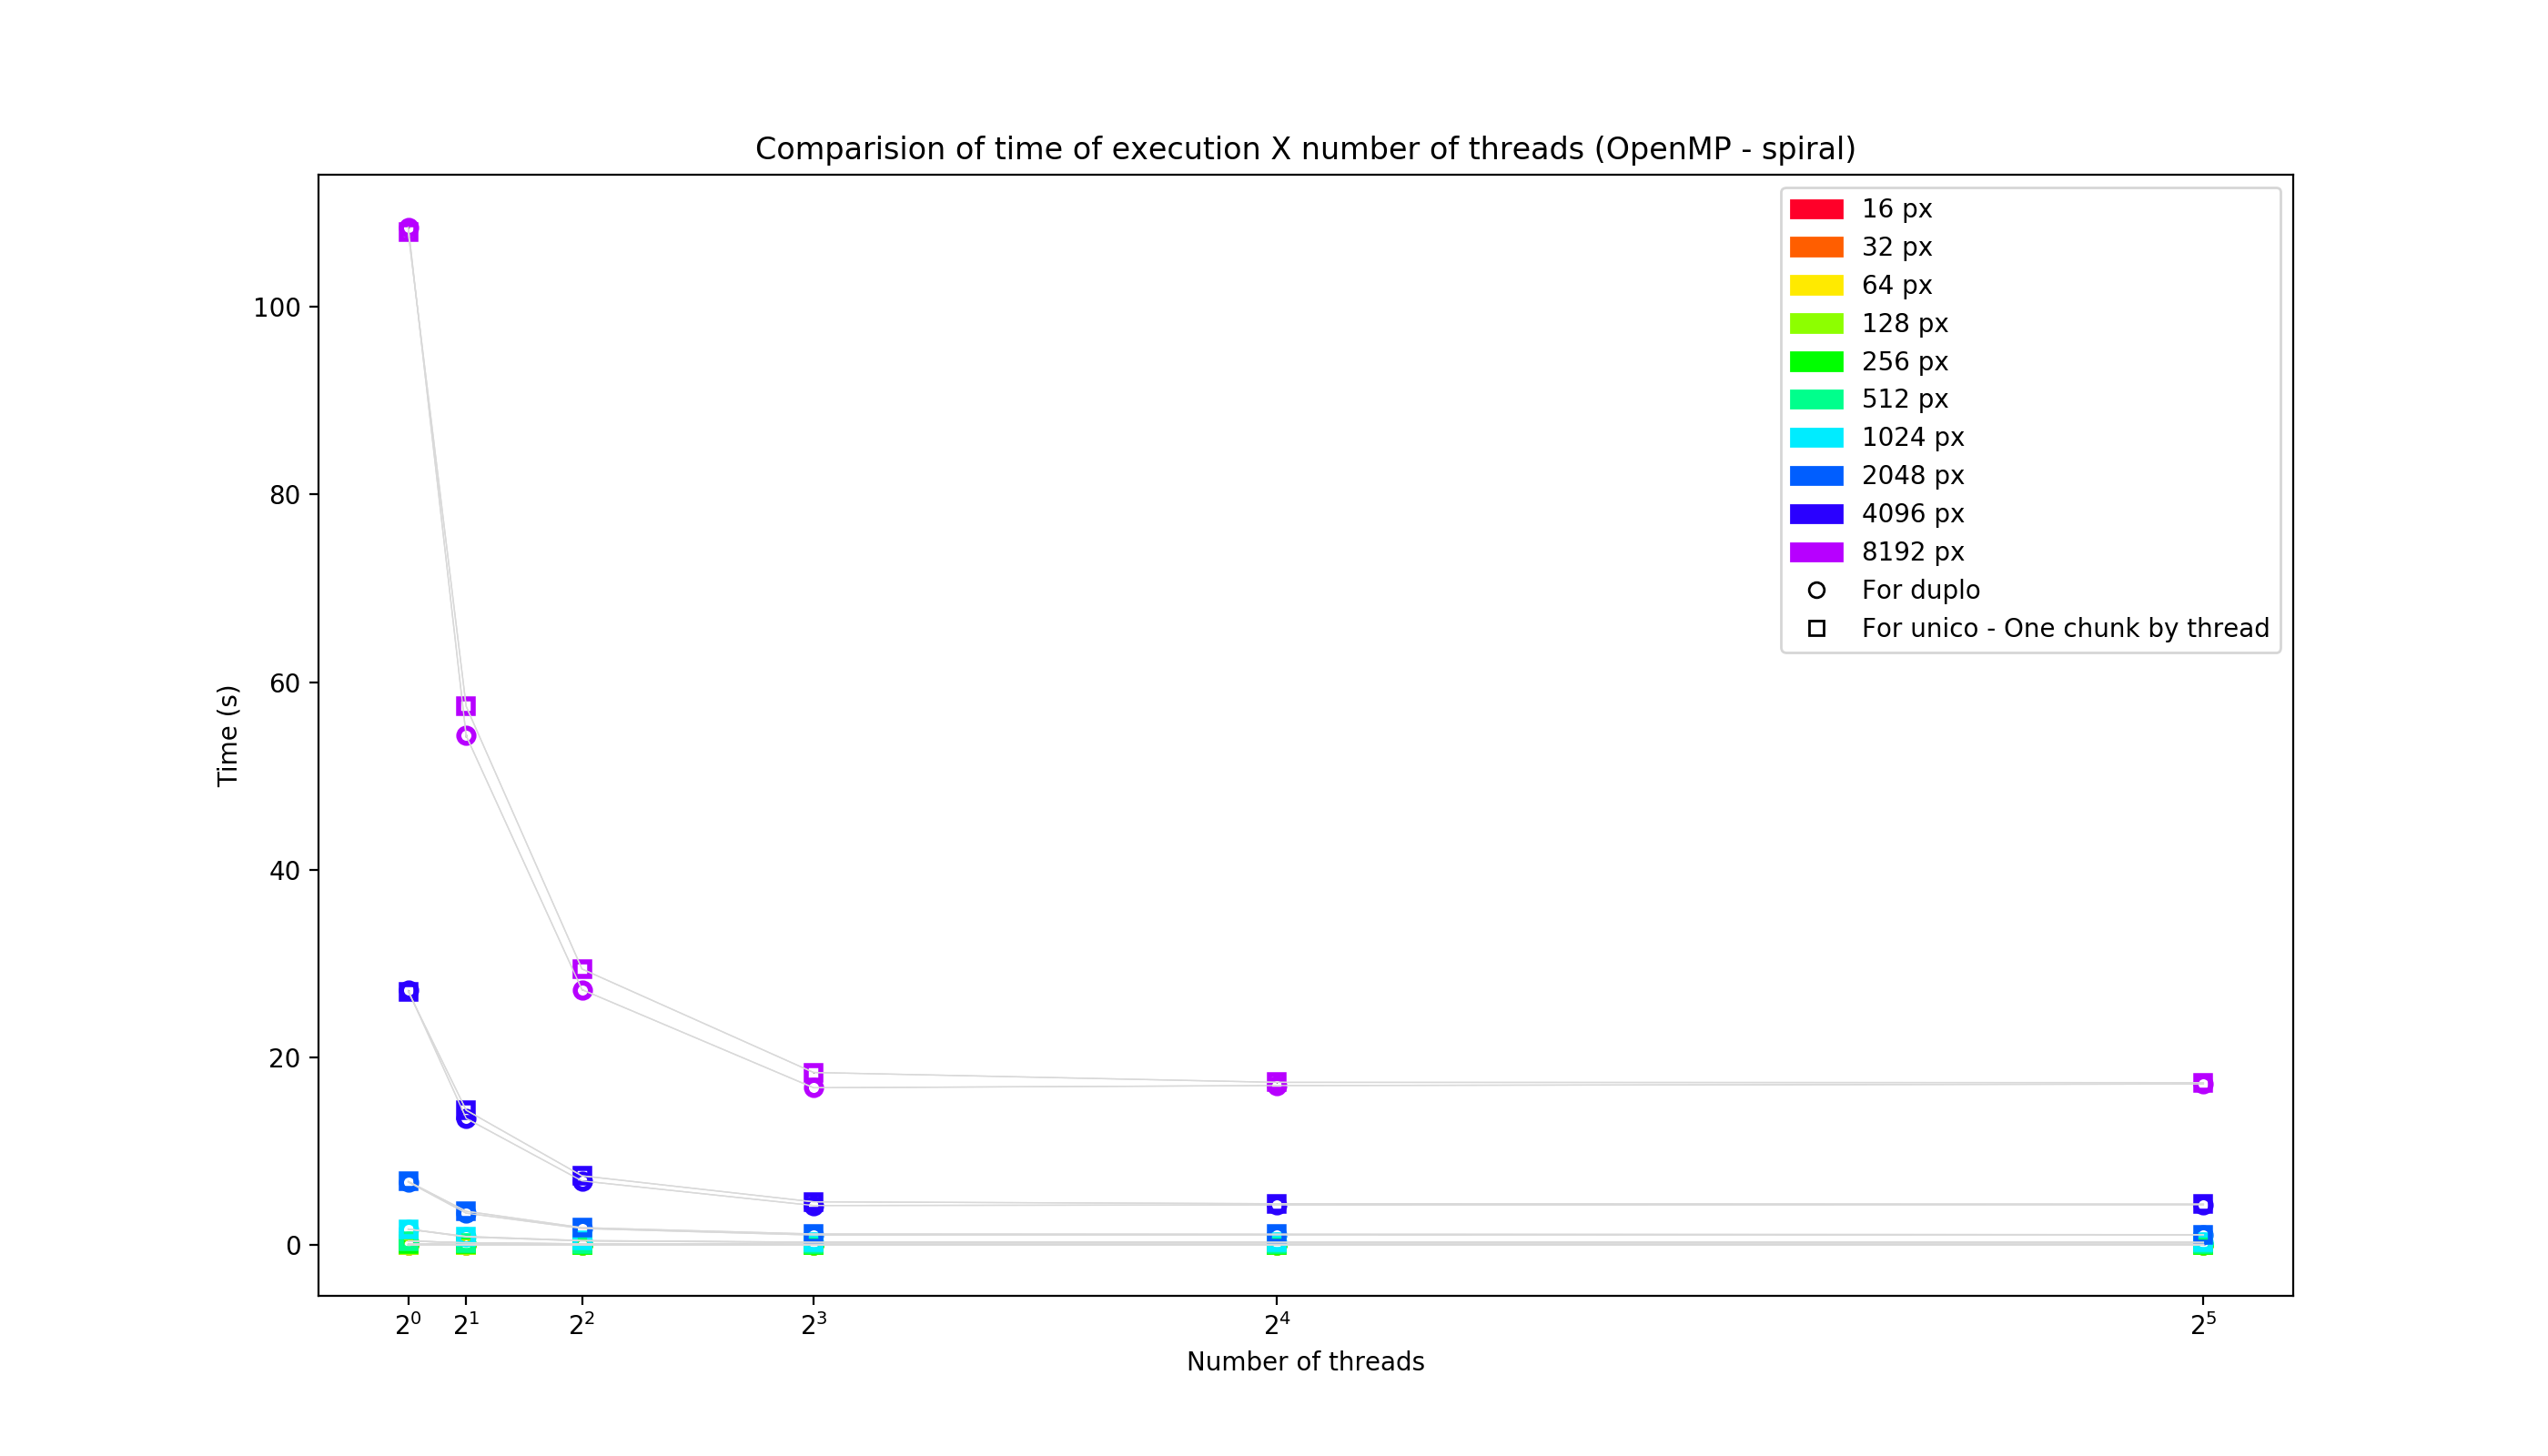
\includegraphics[scale=.55]{for_duploXunico_bigbig/compare_timeXthread_spiral_OpenMPpng.png}}
\end{figure}


%%%%%%%%%%%%%%%%% DISCUSSÂO DOS RESULTADOS %%%%%%%%%%%%%%%%%%%%%%%
\newpage
\section{Discussão dos Resultados}
{\bf Por que é recomendado realizar mais de uma medição?} 
    Porque os resultados observados dependem do estado da máquina
    durante a execução do programa. Como testamos nossos programas
    em máquinas com um sistema operacional, rodando diversos outros
    programas ao mesmo tempo, é esperado que fatores como fila de
    processos, paginação de memória, etc, interfira no tempo de 
    execução do nosso programa. Portanto, se tiramos uma média
    de várias execuções, somos capazes de dizer aproximadamente
    o comportamento médio do programa.

{\bf Por que você acha que existe variabilidade entre execuções do mesmo programa?}

{\bf Como e por que as três versões do programa se comportam com a variação: Do tamanho da entrada? Das regiões do Conjunto de Mandelbrot? Do número de threads?}
As variações de tempo de execução em relação ao tamanho da entrada ocorrem, pois o tamanho do for dentro da função \code{compute\_mandelbrot()} depende do tamanho da entrada. Isto significa que o for será executado mais vezes se o tamanho da entrada for maior e consequentemente levará mais tempo para executar o programa.

As variações causadas pelas diferentes regiões são devido ao maior número de pontos onde há maior número de iterações. Vejamos os histogramas de cada uma das regiões:

\begin{figure}[H]
    \makebox[\textwidth][c]{
        \begin{tabular}{c c}
            \subfigure[] {
                {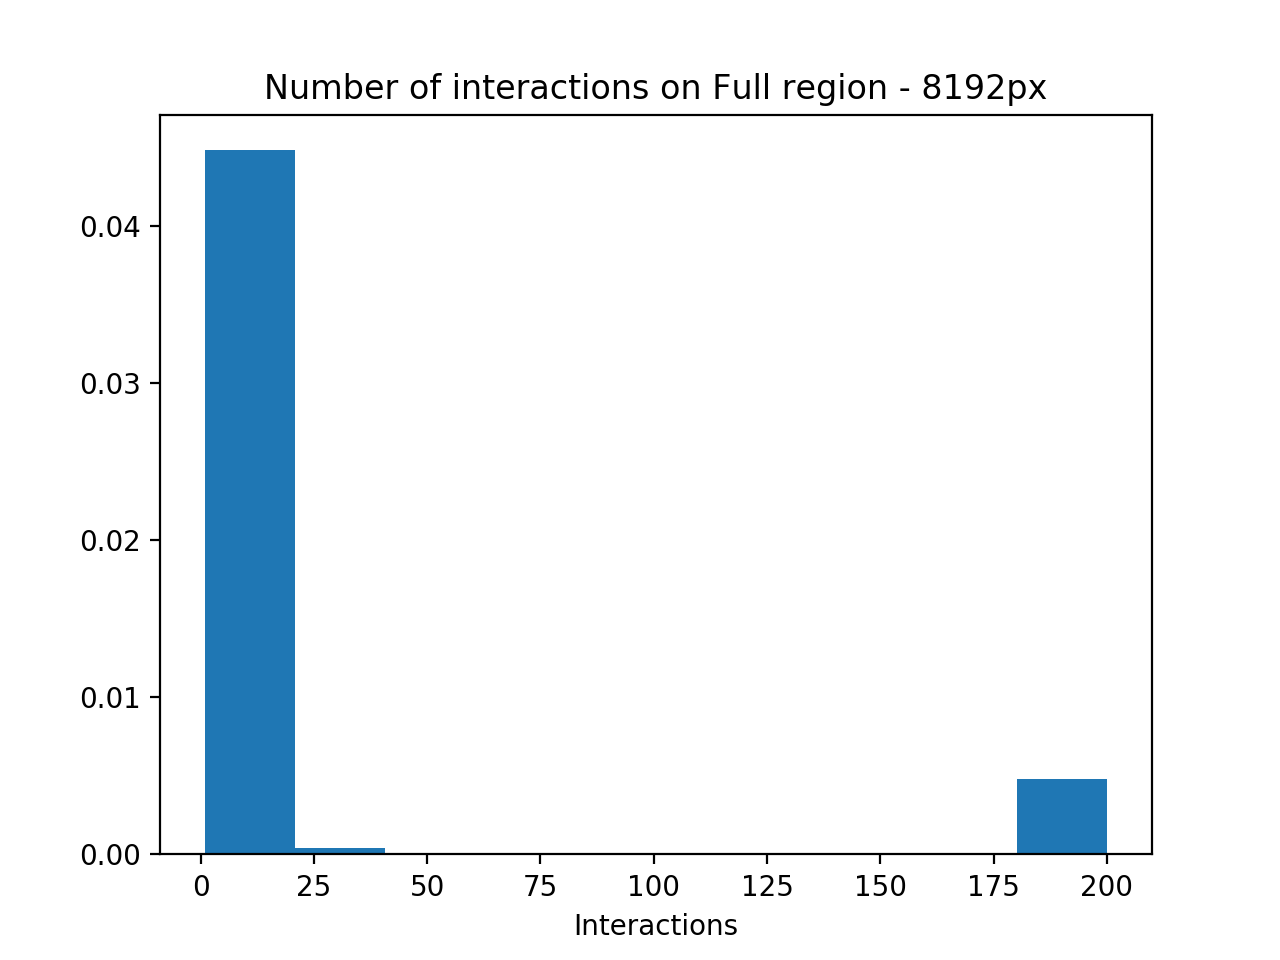
\includegraphics[scale=.55]{hist/full_hist.png}}
            }
            &
            \subfigure[] {
                {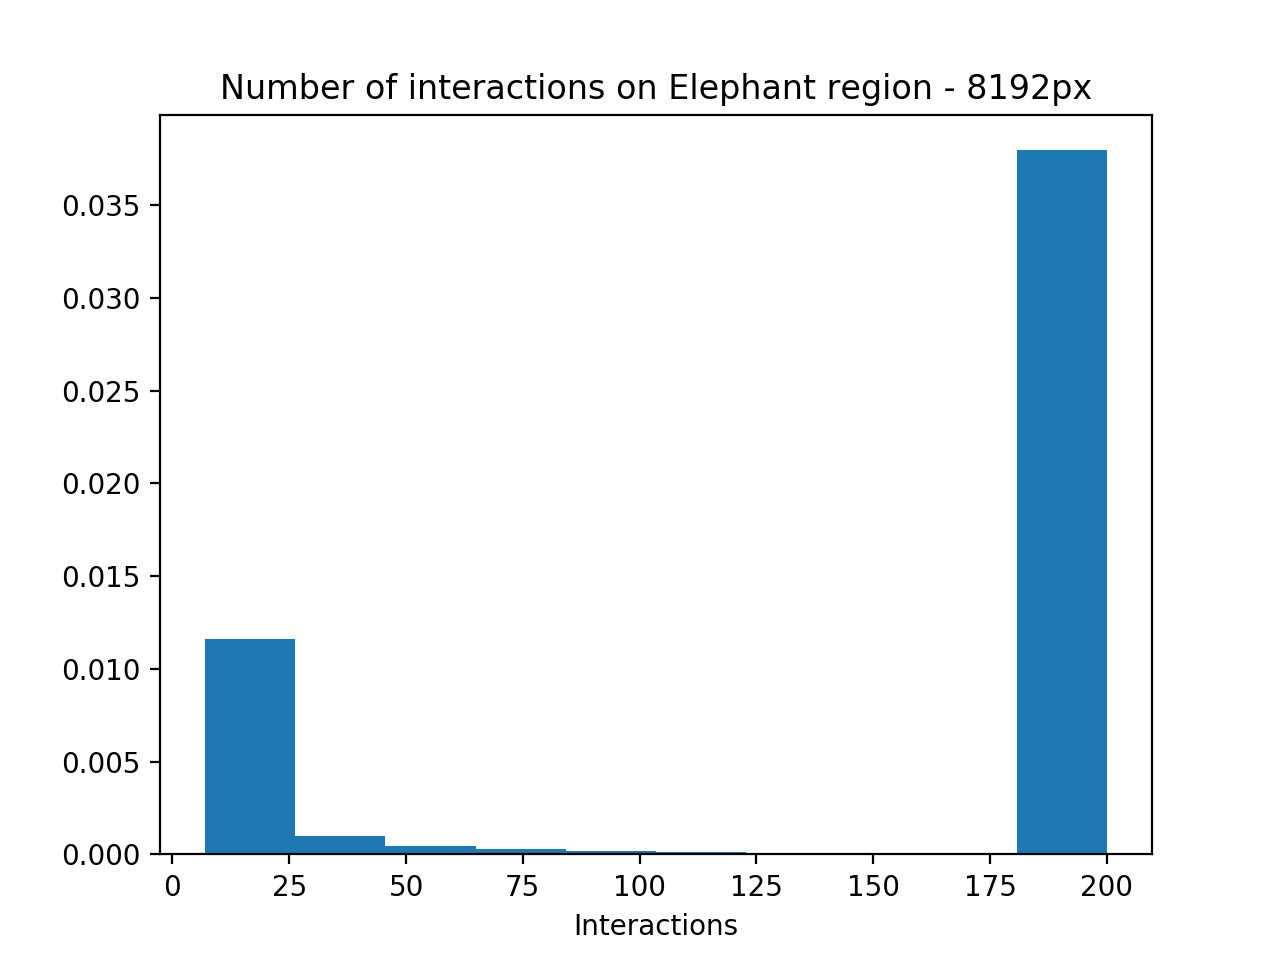
\includegraphics[scale=.55]{hist/elephant_hist.png}}
            }
            \\
            \subfigure[] {
                {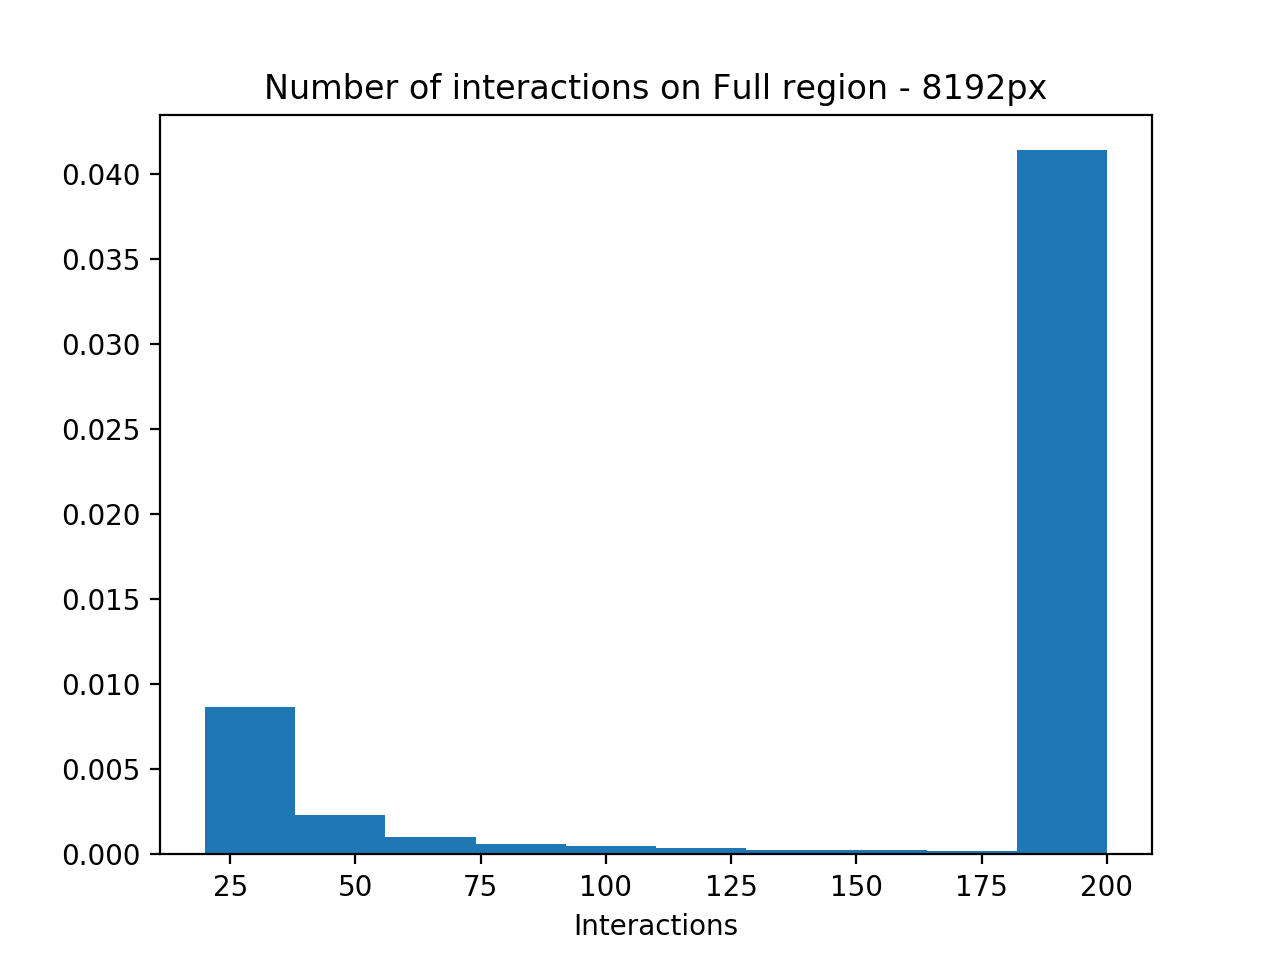
\includegraphics[scale=.55]{hist/seahorse_hist.png}}
            }
            &
            \subfigure[] {
                {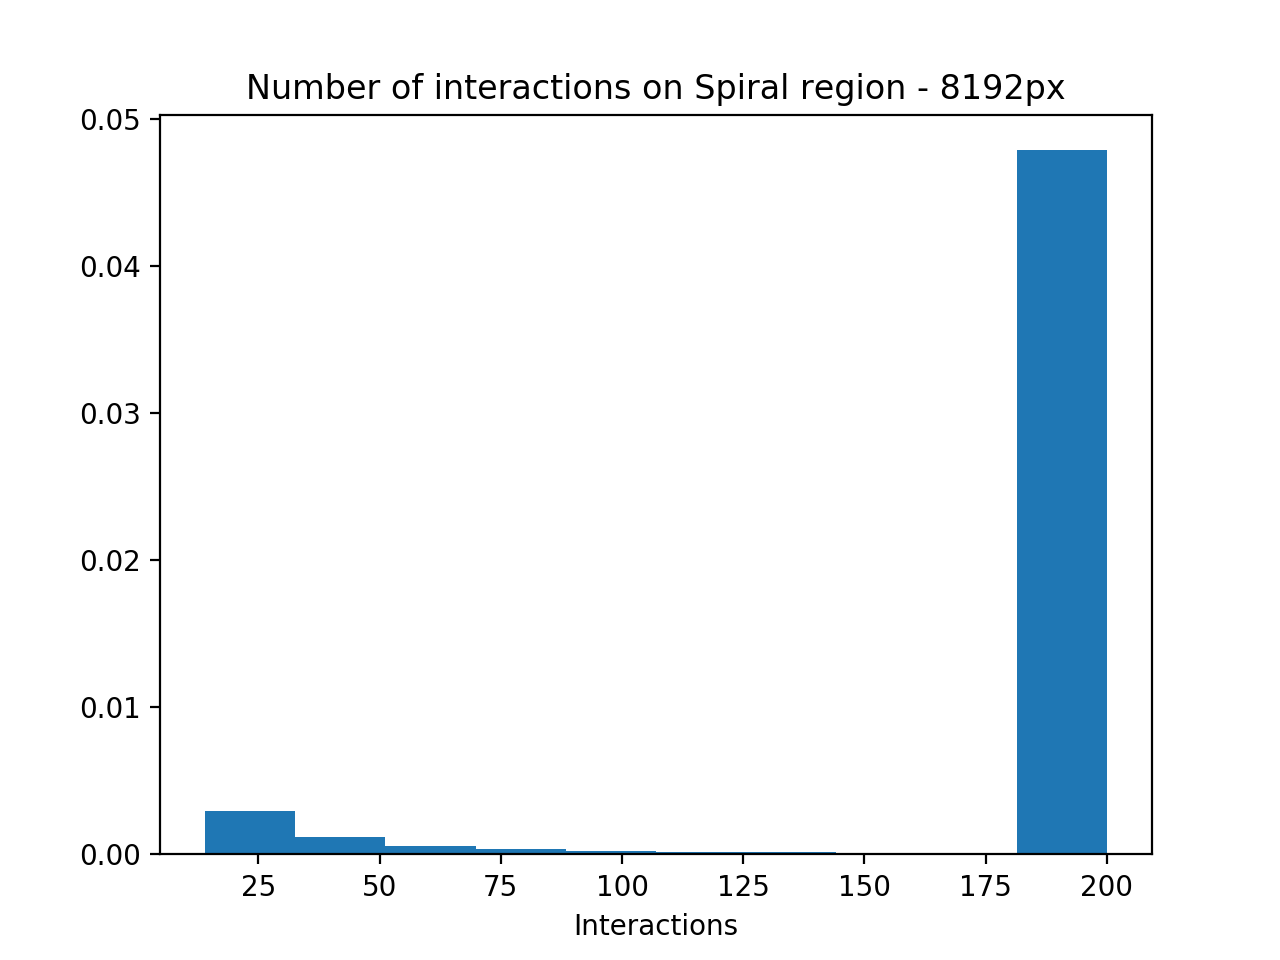
\includegraphics[scale=.55]{hist/spiral_hist.png}}
            }
        \end{tabular}
    }
\end{figure}

Na região Full vemos que a maior parte dos pontos tem poucas iterações do calculo de mandelbrot. A média $\mu = 22.038$ e o desvio padrão $\sigma = 58.217$ comprovam esse fato. Tais valore comparados aos da região Elephant ($\mu = 151.757$, $\sigma = 80.798$), Seahorse ($\mu = 160.667$, $\sigma = 69.371$) e Spiral ($\mu = 183.204$, $\sigma = 49.430$) nos mostram porquê os calculos das regiões, Elephant, Seahorse e Spiral levaram mais tempo. Como nessas regiões há mais iterações em geral, mais tempo é gasto calculando. Isso é multiplicado por cada ponto, o que causa um bom atraso na execução do programa. 


DO NUMERO DE THREADS <<< AQUI ESTRELINHA AQUIIIIII

{\bf Qual o impacto das operações de I/O e alocação de memória no tempo de execução?}
Vimos na analise da implementação sequencial que as operações de leitura e escrita e a alocação da memória afetam consideravelmente o desempenho. Gostariamos de ver qual foi a diferença entre a implementação com operações de I/O e com alocação em relação à sem ambos. Se pudermos tomar essa diferença teremos uma estimativa do tempo que leva as operações I/O e alocação:


\begin{figure}[H]
    \makebox[\textwidth][c]{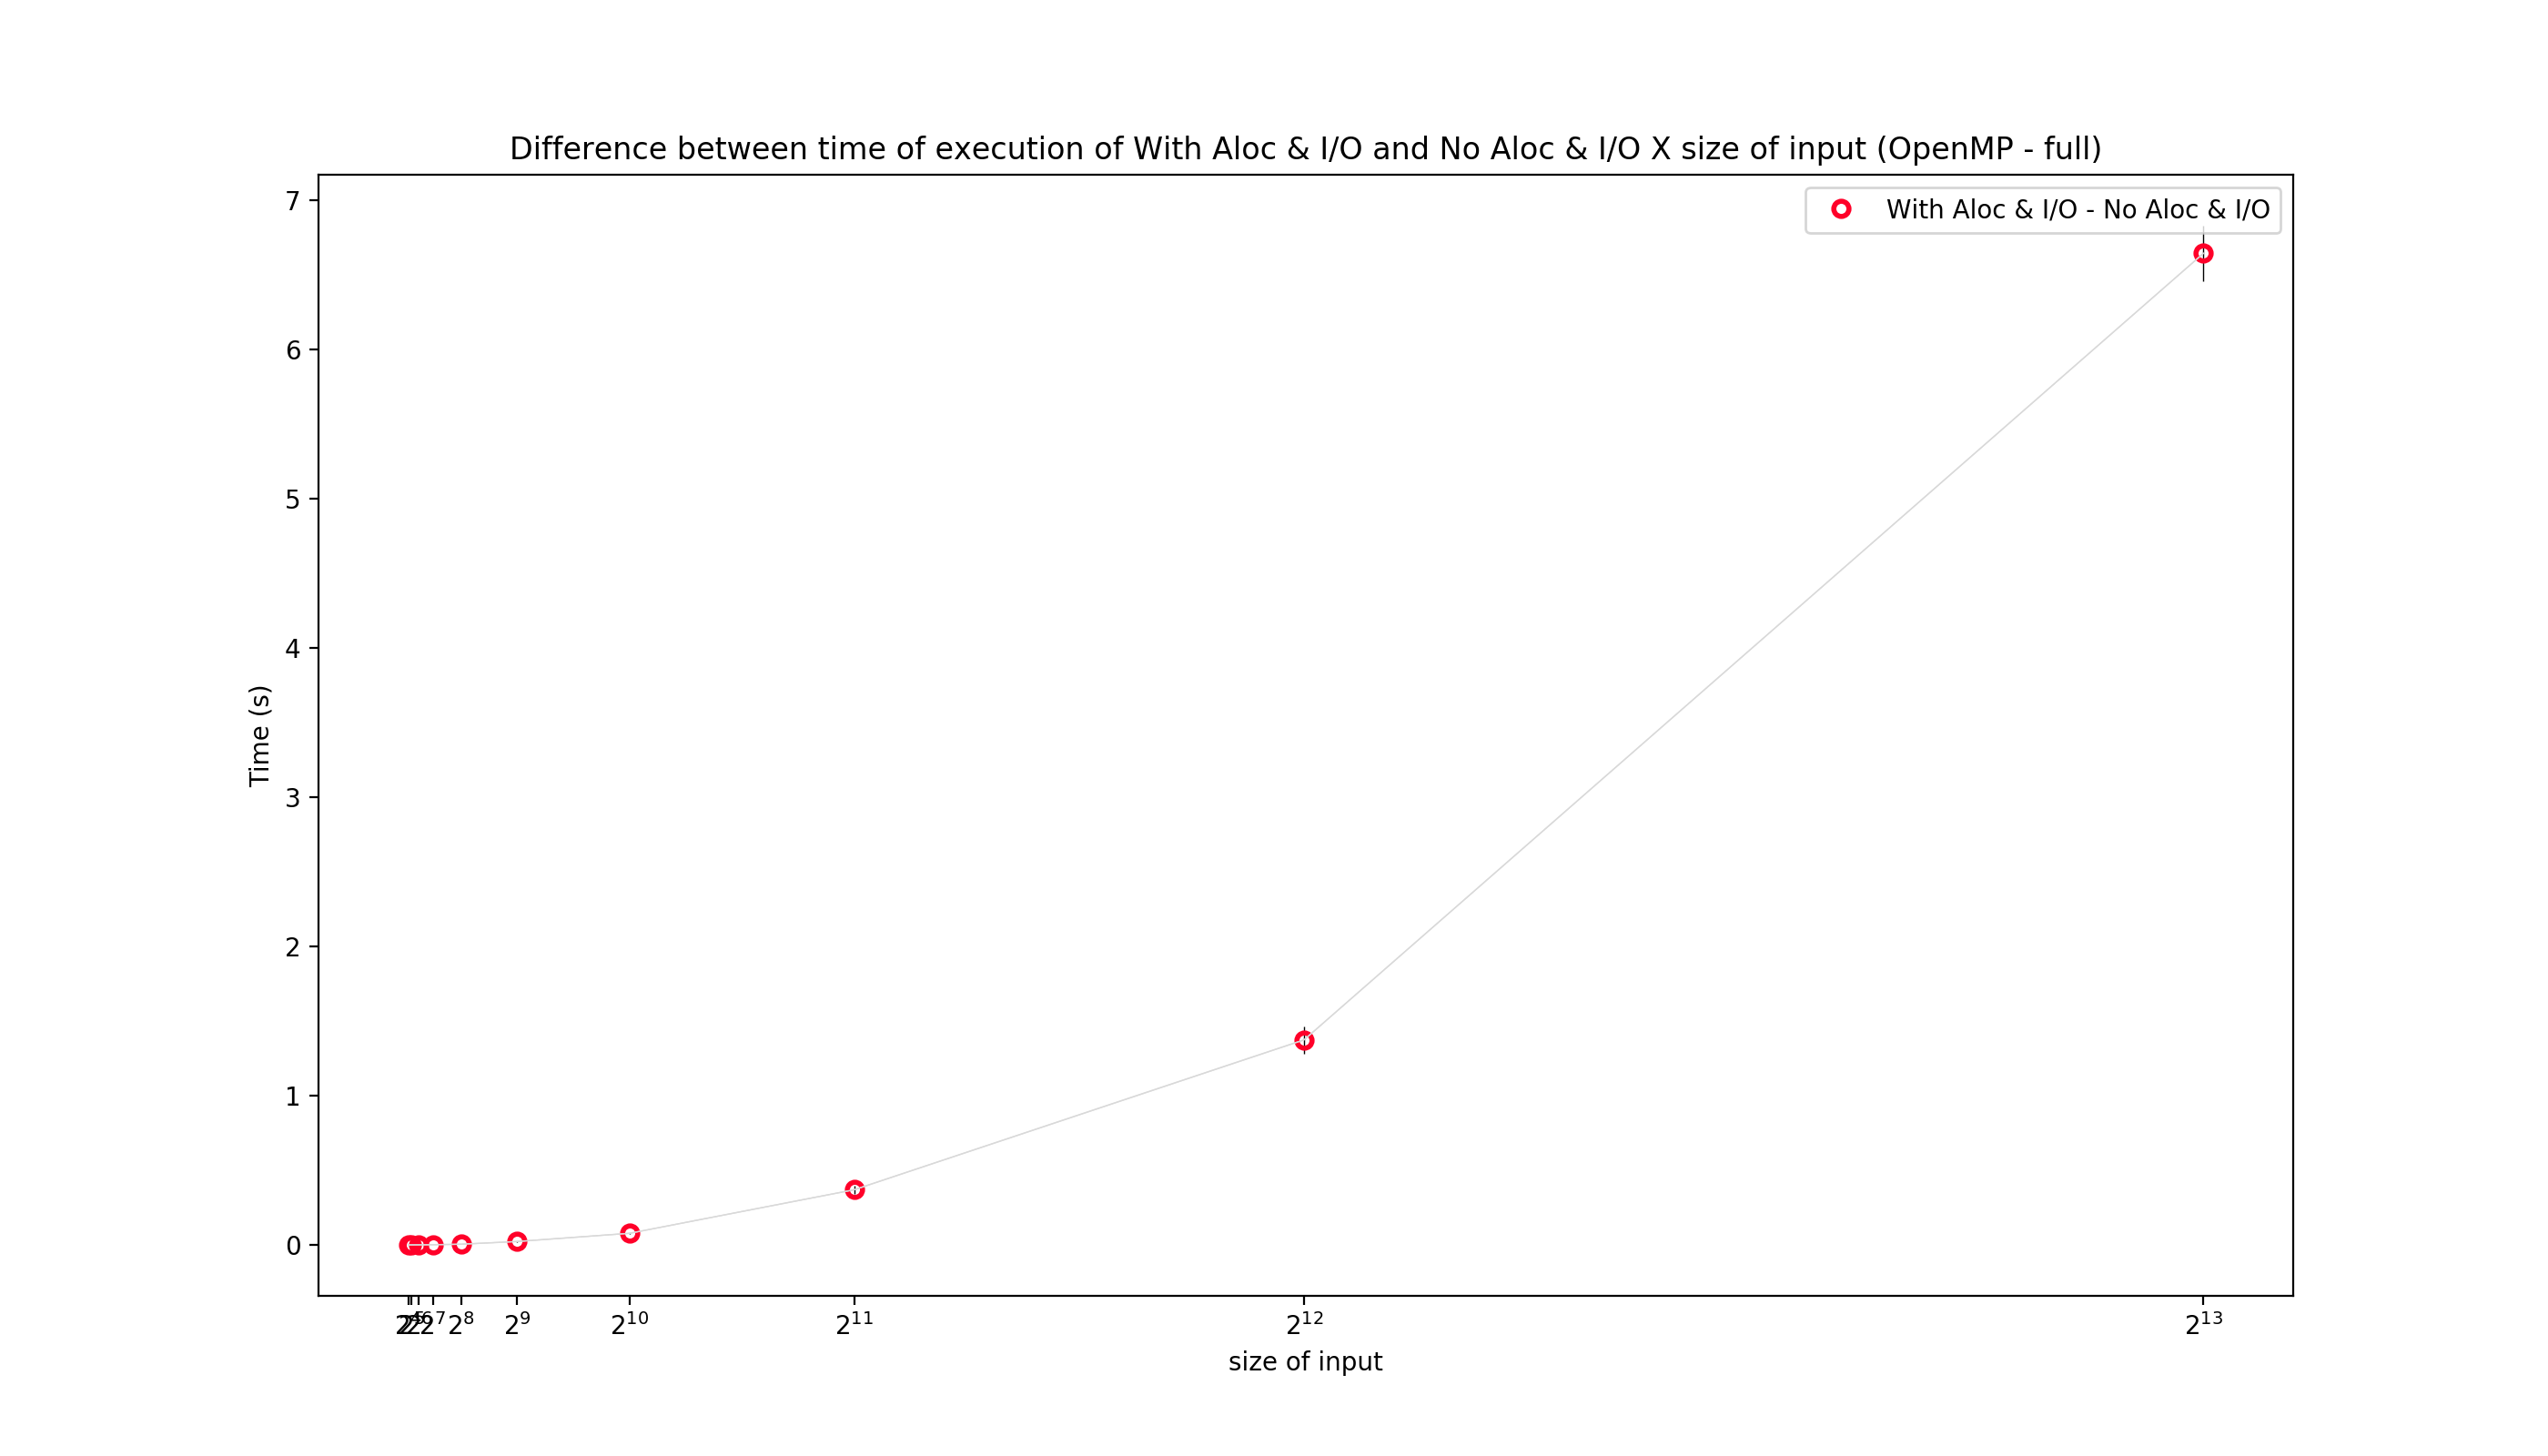
\includegraphics[scale=.55]{seq_comp/difference_timeXsize_full_OpenMPpng.png}}
\end{figure}

Nota-se que o tempo levado pelas operações de I/O e alocação dinamica tem comportamento exponencial em relação ao tamanho da entrada. Vale lembrar que o tamanho da entrada é somente o lado da imagem, portanto o tamanho da matriz a ser alocada também é exponencial em relação ao tamanho da entrada. Para as demais regiões nota-se um comportamento semelhante:

\begin{figure}[H]
    \makebox[\textwidth][c]{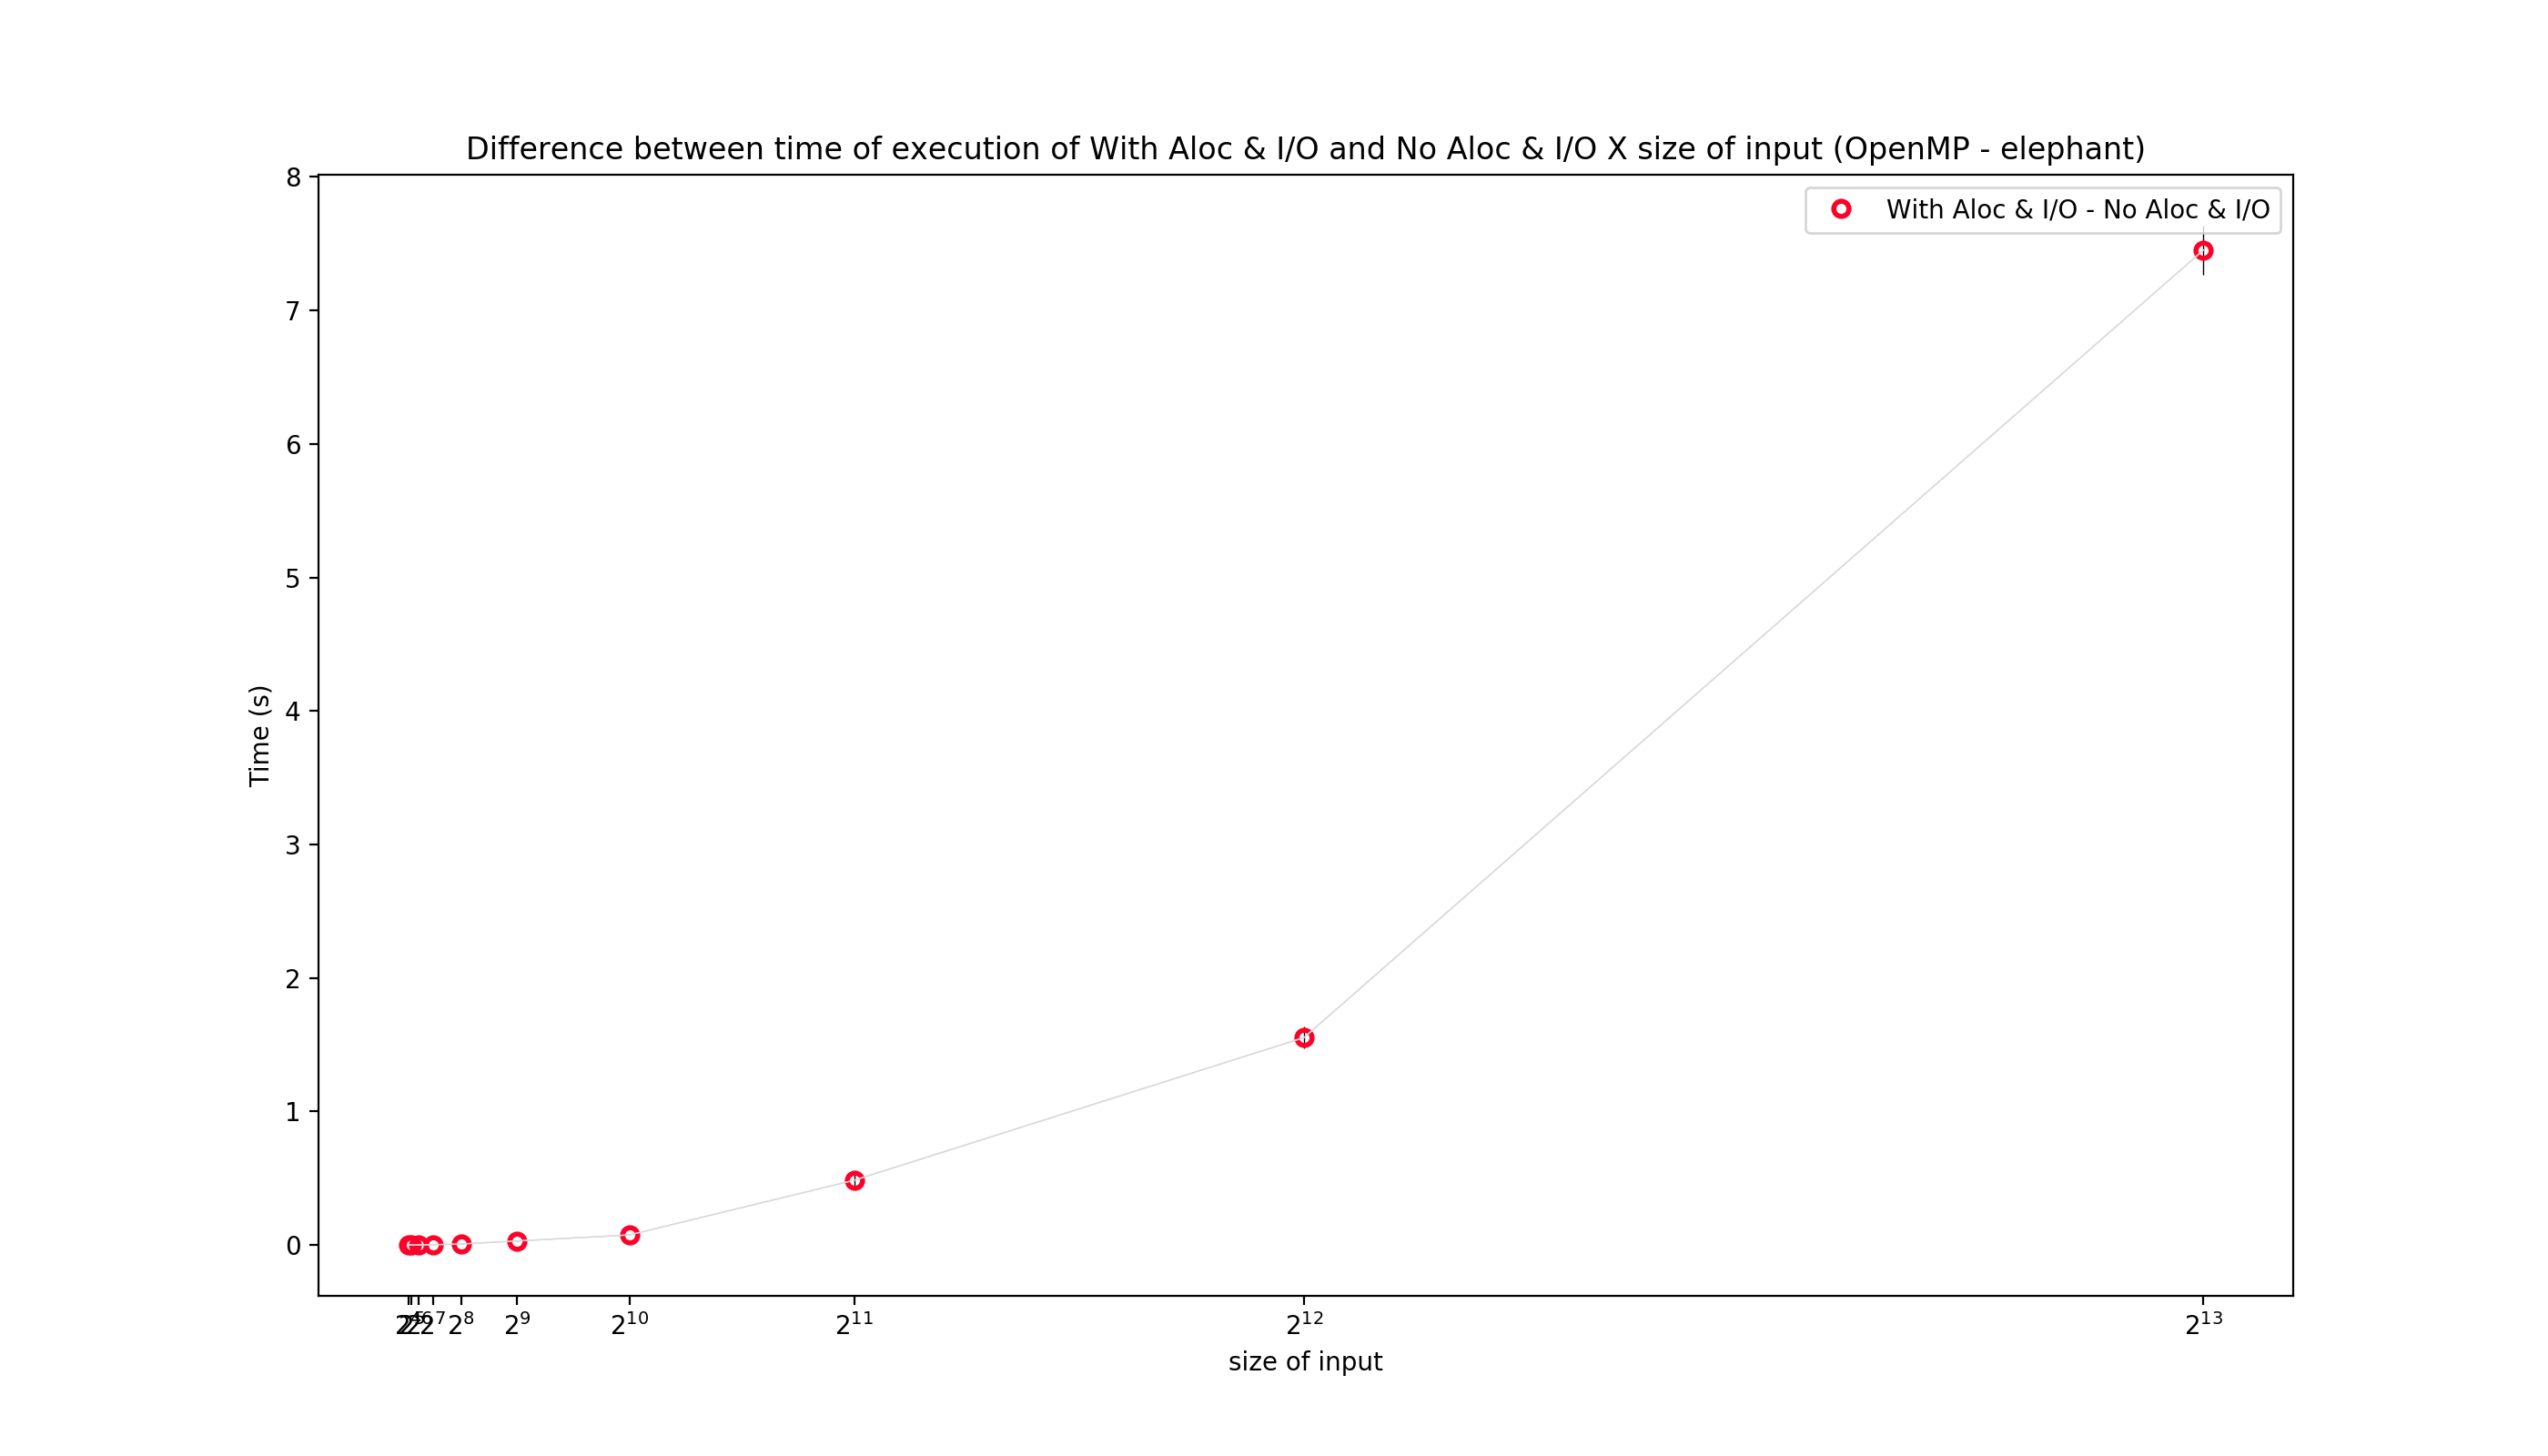
\includegraphics[scale=.55]{seq_comp/difference_timeXsize_elephant_OpenMPpng.png}}
\end{figure}
\begin{figure}[H]
    \makebox[\textwidth][c]{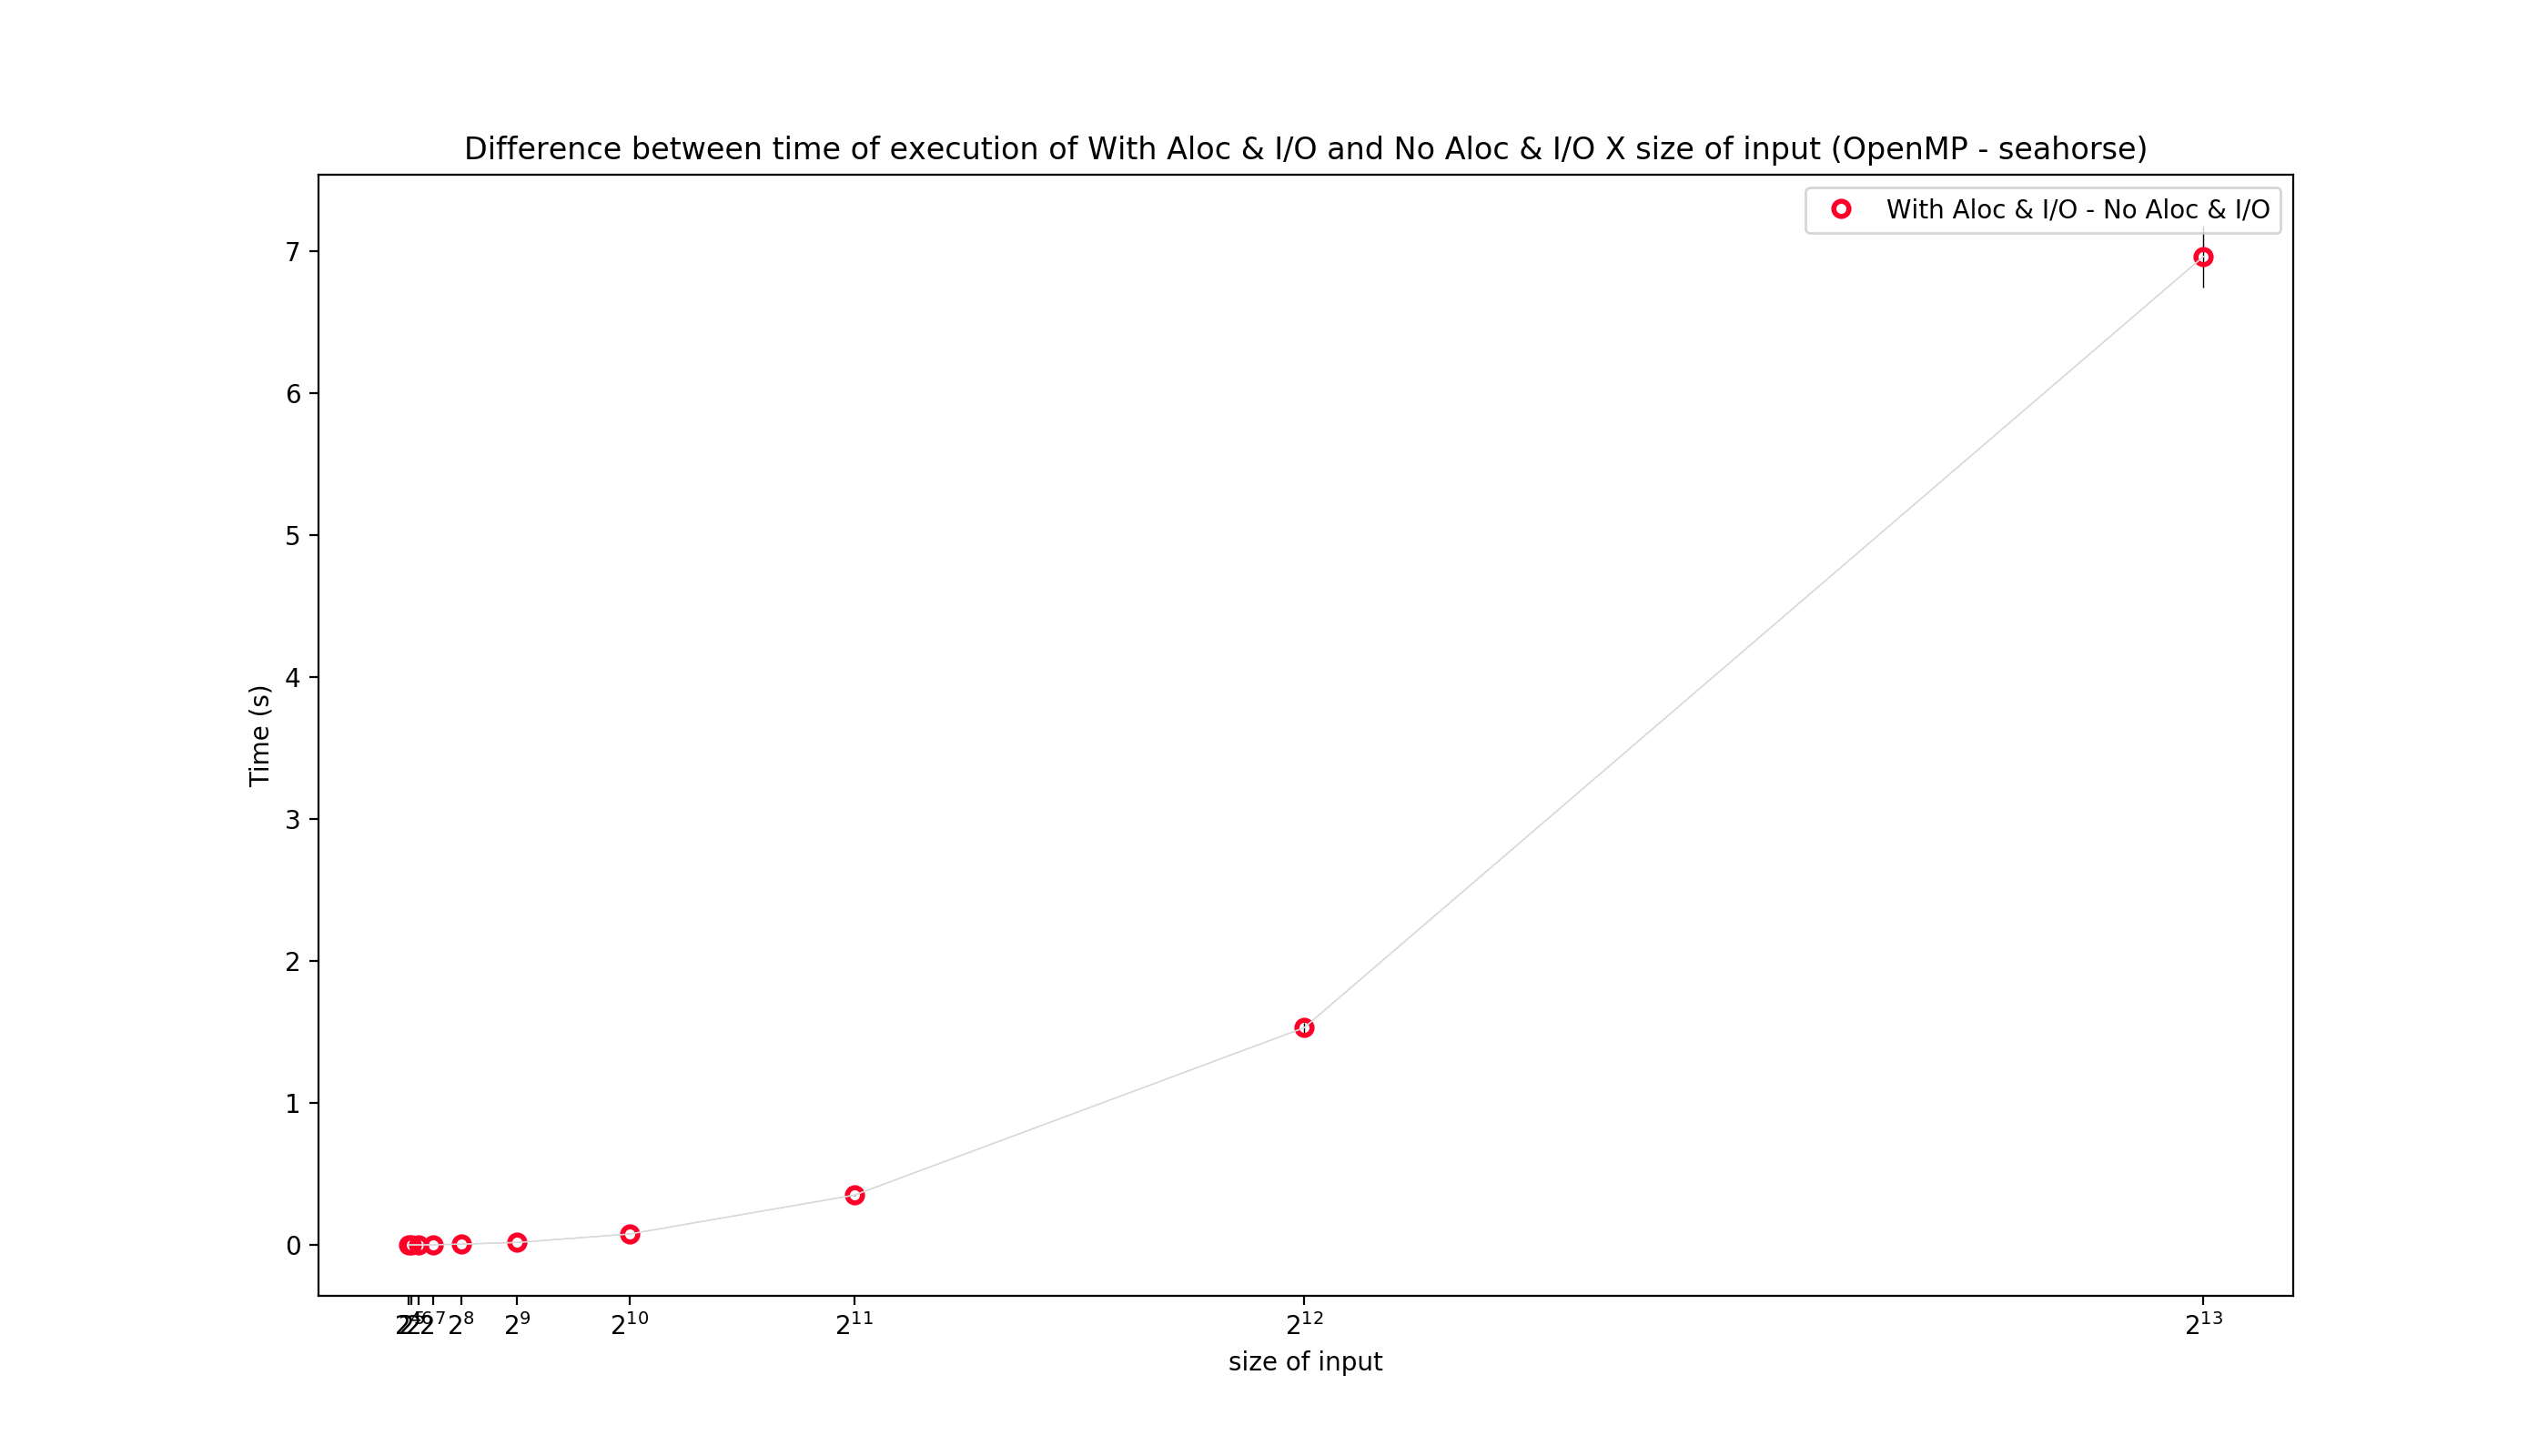
\includegraphics[scale=.55]{seq_comp/difference_timeXsize_seahorse_OpenMPpng.png}}
\end{figure}
\begin{figure}[H]
    \makebox[\textwidth][c]{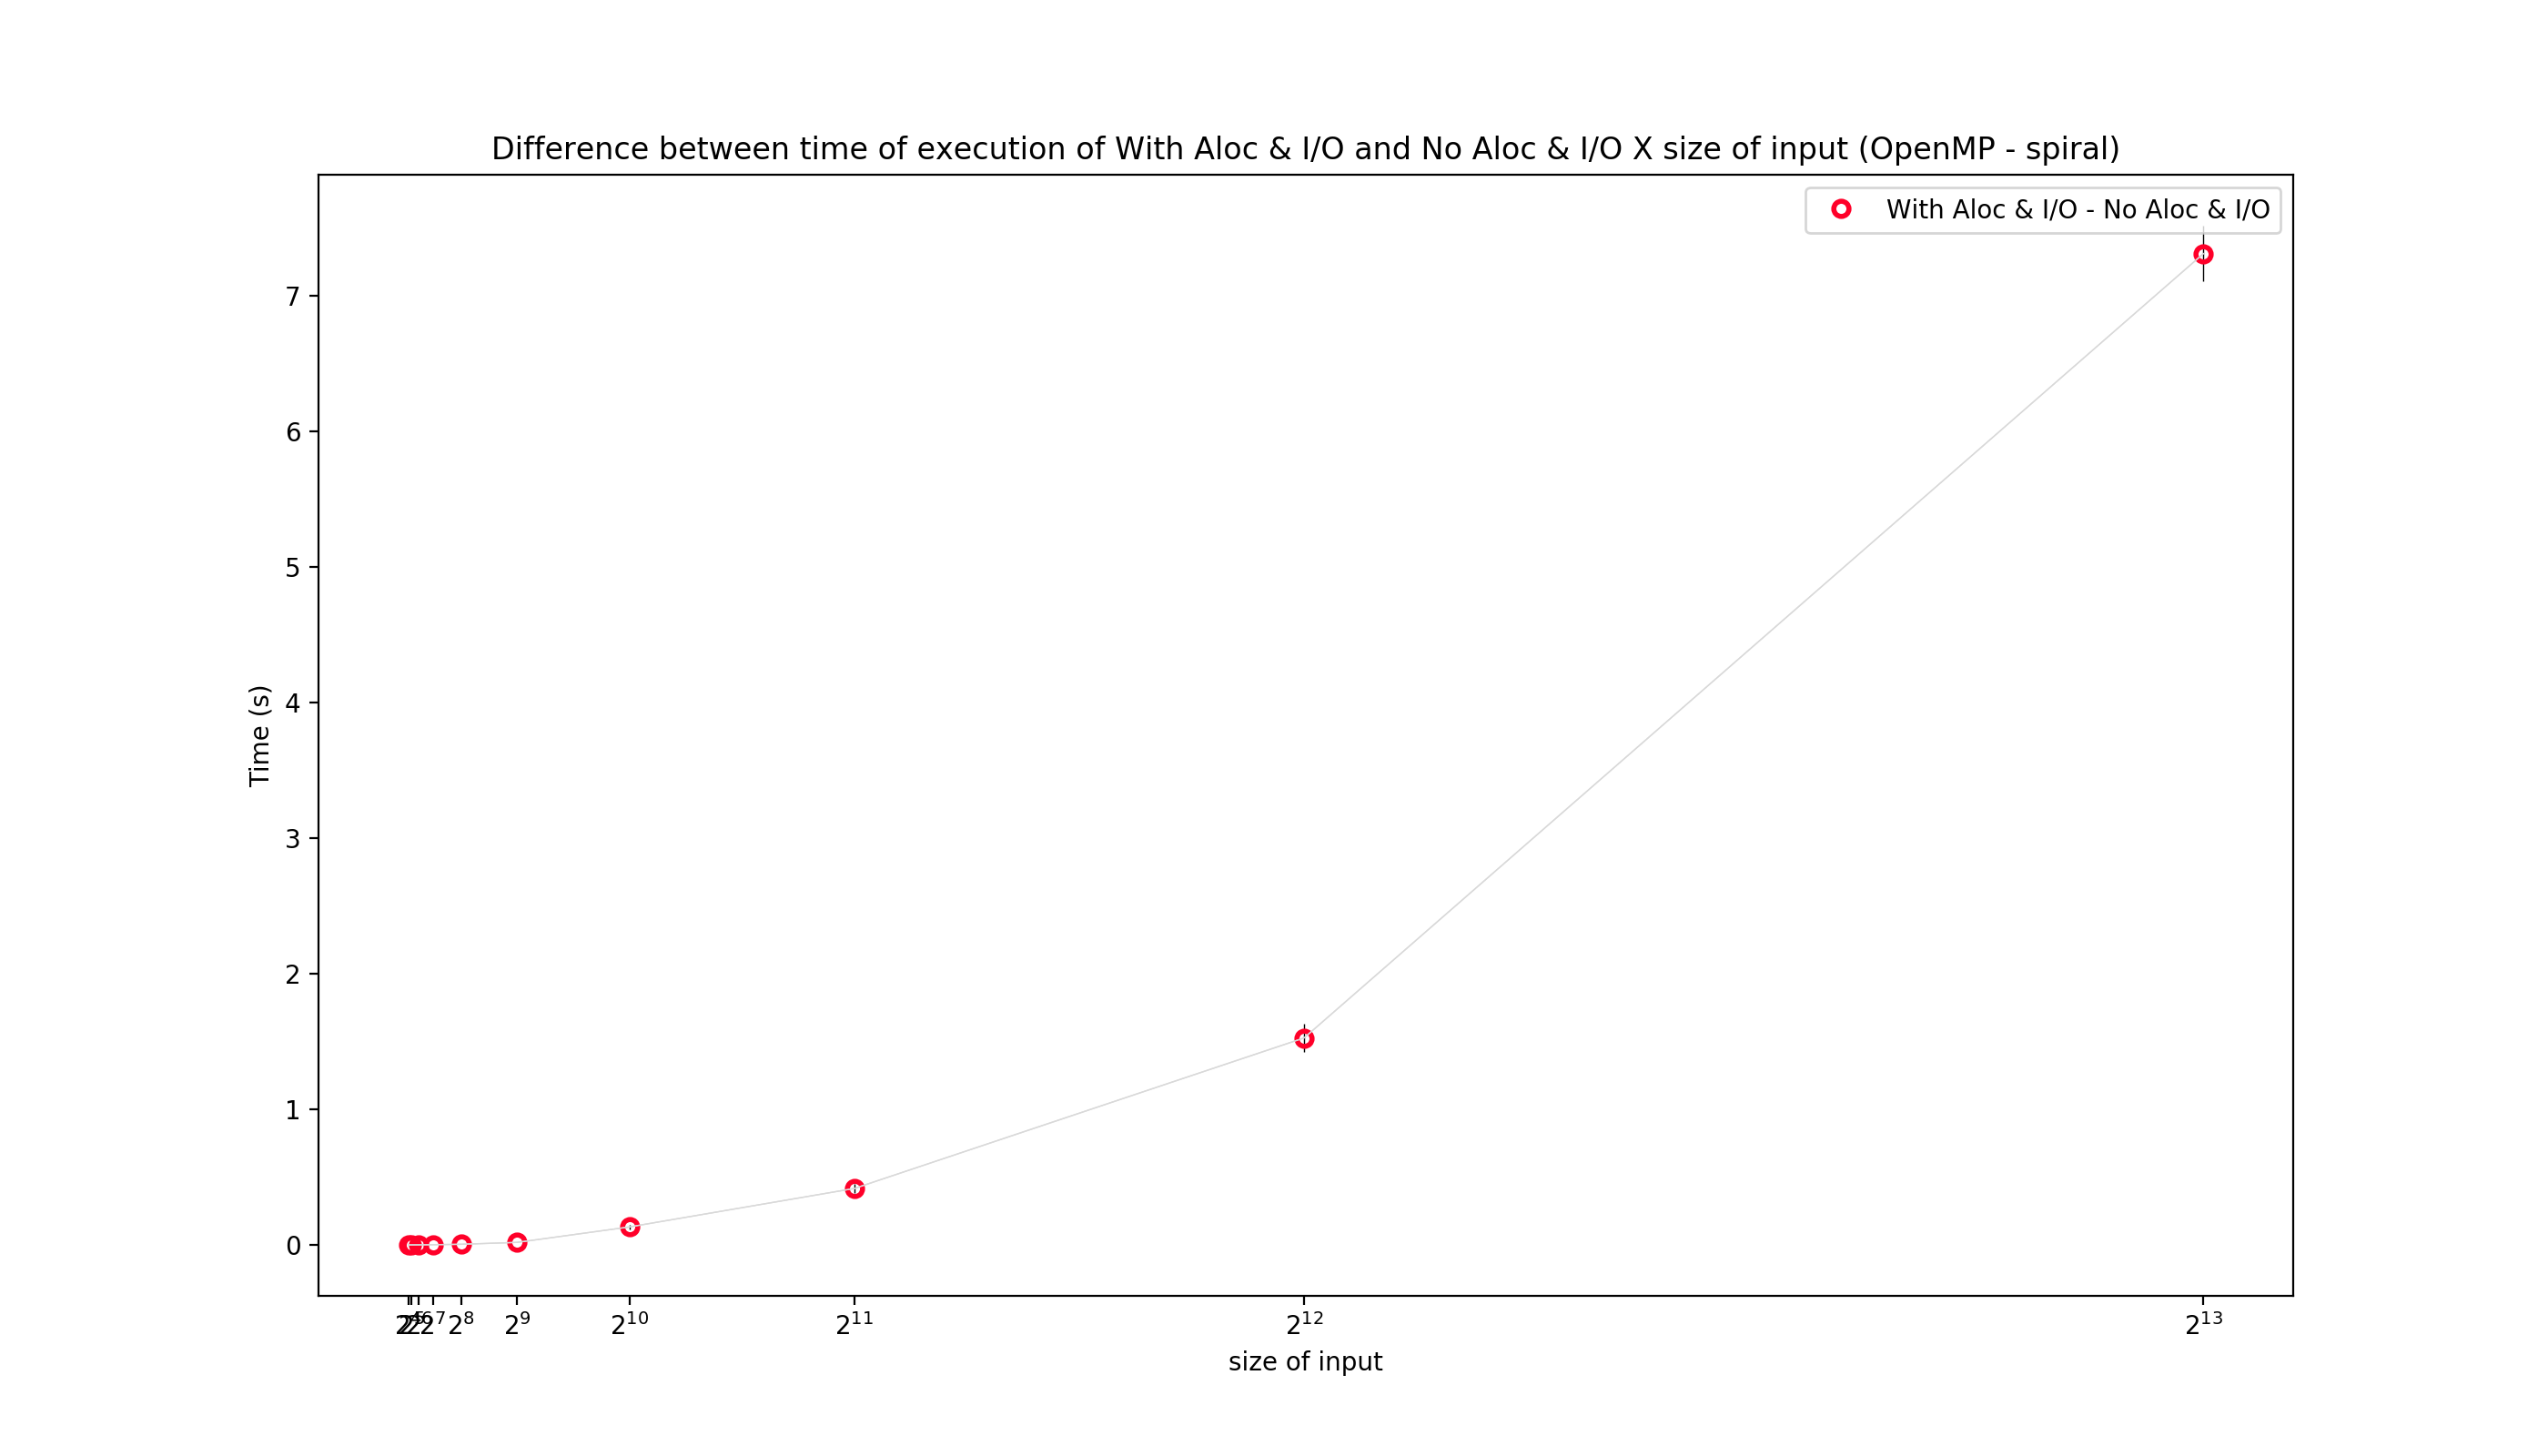
\includegraphics[scale=.55]{seq_comp/difference_timeXsize_spiral_OpenMPpng.png}}
\end{figure}

Notemos ainda que os valores também são semelhantes, independente da região. Como explicado anteriormente, isso se deve ao fato de que as operações de I/O e a alocação de memória independem do número de iterações do cálculo de mandelbrot em cada ponto.


\newpage
\section{Conclusão}
\newpage

\end{document}
